\cotefile{148}
\scanpage{29}
\margin{\(M_{0,5}\;-\)}

\diagram{\[\begin{array}{ll}
\texttt{\unsure{GGGGGGGGGG}}&\texttt{\unsure{UU}\qquad\unsure{UU}}\\
\texttt{\unsure{GGGGGGGGGG}}&\texttt{\unsure{UU}\qquad\unsure{UU}}\\
\texttt{GG\qquad GG}&\texttt{UU\qquad U}\\
\texttt{GG}&\texttt{UU\qquad U}\\
\texttt{GG}&\texttt{\unsure{UU}\qquad\unsure{U}}\\
\texttt{GG}&\texttt{UU\qquad U}\\
\texttt{GG\quad GGGGG}&\texttt{UU\qquad U}\\
\texttt{GG\quad GGGGG}&\texttt{\unsure{UU}\qquad\unsure{U}}\\
\texttt{GG\qquad GG}&\texttt{UU\qquad U}\\
\texttt{GG\qquad GG}&\texttt{UU\qquad U}\\
\texttt{\unsure{GGGGGGGGGG}}&\texttt{\unsure{UUUUUUUUUU}}\\
\texttt{\unsure{GGGGGGGGGG}}&\texttt{\unsure{UUUUUUUUUU}}
\end{array}\]}

\diagram{\[\begin{array}{lllll}
\texttt{****\unsure{P}}&\texttt{START}&\texttt{\unsure{STC|STG} 55 GUTS}&\texttt{ROOM}\\
\texttt{****\unsure{P}}&\texttt{START}&\texttt{\unsure{STC|STG} 55 GUTS}&\texttt{ROOM}\\
\texttt{****\unsure{P}}&\texttt{START}&\texttt{\unsure{STC|STG} 55 GUTS}&\texttt{ROOM}\\
\texttt{****\unsure{P}}&\texttt{START}&\texttt{\unsure{STC|STG} 55 GUTS}&\texttt{ROOM}\\
\texttt{****\unsure{P}}&\texttt{START}&\texttt{\unsure{STC|STG} 55 GUTS}&\texttt{ROOM}\\
\texttt{****\unsure{P}}&\texttt{START}&\texttt{\unsure{STC|STG} 55 GUTS}&\texttt{ROOM}
\end{array}\]}

\texttt{0DERNIERE MISE A JOUR DE JOURNAL: 01-06-82}\\
\texttt{STAGE FORMATION \unsure{NLT-CLOTILDE} LES 22 ET 23 JUIN}

\mspage{28}
\scanpage{30}
\texttt{//*\quad GUTS\quad 0055\qquad I}

\diagram{\[\begin{array}{llll}
\texttt{\ GGGGGGGGGG\ } & \texttt{UU\ \ \ \ \ \ \ \ UU} & \texttt{TTTTTTTTTTTT} & \texttt{\ SSSSSSSSSS\ }\\
\texttt{GGGGGGGGGGGG} & \texttt{UU\ \ \ \ \ \ \ \ UU} & \texttt{TTTTTTTTTTTT} & \texttt{SSSSSSSSSSSS}\\
\texttt{GG\ \ \ \ \ \ \ \ GG} & \texttt{UU\ \ \ \ \ \ \ \ UU} & \texttt{\ \ \ \ \ TT\ \ \ \ \ } & \texttt{SS\ \ \ \ \ \ \ \ SS}\\
\texttt{GG\ \ \ \ \ \ \ \ \ \ } & \texttt{UU\ \ \ \ \ \ \ \ UU} & \texttt{\ \ \ \ \ TT\ \ \ \ \ } & \texttt{SS\ \ \ \ \ \ \ \ \ \ }\\
\texttt{GG\ \ \ \ \ \ \ \ \ \ } & \texttt{UU\ \ \ \ \ \ \ \ UU} & \texttt{\ \ \ \ \ TT\ \ \ \ \ } & \texttt{SSS\ \ \ \ \ \ \ \ \ }\\
\texttt{GG\ \ \ \ \ \ \ \ \ \ } & \texttt{UU\ \ \ \ \ \ \ \ UU} & \texttt{\ \ \ \ \ TT\ \ \ \ \ } & \texttt{\ SSSSSSSSS\ \ }\\
\texttt{GG\ \ \ \ \ GGGGG} & \texttt{UU\ \ \ \ \ \ \ \ UU} & \texttt{\ \ \ \ \ TT\ \ \ \ \ } & \texttt{\ \ SSSSSSSSS\ }\\
\texttt{GG\ \ \ \ \ GGGGG} & \texttt{UU\ \ \ \ \ \ \ \ UU} & \texttt{\ \ \ \ \ TT\ \ \ \ \ } & \texttt{\ \ \ \ \ \ \ \ \ SSS}\\
\texttt{GG\ \ \ \ \ \ \ \ GG} & \texttt{UU\ \ \ \ \ \ \ \ UU} & \texttt{\ \ \ \ \ TT\ \ \ \ \ } & \texttt{\ \ \ \ \ \ \ \ \ \ SS}\\
\texttt{GG\ \ \ \ \ \ \ \ GG} & \texttt{UU\ \ \ \ \ \ \ \ UU} & \texttt{\ \ \ \ \ TT\ \ \ \ \ } & \texttt{SS\ \ \ \ \ \ \ \ SS}\\
\texttt{GGGGGGGGGGGG} & \texttt{UUUUUUUUUUUU} & \texttt{\ \ \ \ \ TT\ \ \ \ \ } & \texttt{SSSSSSSSSSSS}\\
\texttt{\ GGGGGGGGGG\ } & \texttt{\ UUUUUUUUUU\ } & \texttt{\ \ \ \ \ TT\ \ \ \ \ } & \texttt{\ SSSSSSSSSS\ }
\end{array}\]}

\diagram{\[\begin{array}{lllllllll}
\texttt{****P} & \texttt{START STC 55 GUTS} & \texttt{ROOM} & \texttt{10.32.28 AM 09 JUN 82} & \texttt{R6.PR1} & \texttt{SYS JES2} & \texttt{STC 55 START} & \texttt{P****}\\
\texttt{****P} & \texttt{START STC 55 GUTS} & \texttt{ROOM} & \texttt{10.32.28 AM 09 JUN 82} & \texttt{R6.PR1} & \texttt{SYS JES2} & \texttt{STC 55 START} & \texttt{P****}\\
\texttt{****P} & \texttt{START STC 55 GUTS} & \texttt{ROOM} & \texttt{10.32.28 AM 09 JUN 82} & \texttt{R6.PR1} & \texttt{SYS JES2} & \texttt{STC 55 START} & \texttt{P****}\\
\texttt{****P} & \texttt{START STC 55 GUTS} & \texttt{ROOM} & \texttt{10.32.28 AM 09 JUN 82} & \texttt{R6.PR1} & \texttt{SYS JES2} & \texttt{STC 55 START} & \texttt{P****}\\
\texttt{****P} & \texttt{START STC 55 GUTS} & \texttt{ROOM} & \texttt{10.32.28 AM 09 JUN 82} & \texttt{R6.PR1} & \texttt{SYS JES2} & \texttt{STC 55 START} & \texttt{P****}\\
\texttt{****P} & \texttt{START STC 55 GUTS} & \texttt{ROOM} & \texttt{10.32.28 AM 09 JUN 82} & \texttt{R6.PR1} & \texttt{SYS JES2} & \texttt{STC 55 START} & \texttt{P****}
\end{array}\]}

\texttt{DERNIERE MISE A JOUR DE JOURNAL: 08-06-82}\\
\texttt{STAGE FORMATION NLT-CLOTILDE LES 22 ET 23 JUIN}

\mspage{29}
\scanpage{31}
\margin{\figure{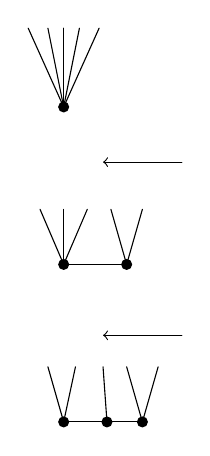
\begin{tikzpicture}[x=1cm,y=1cm,line cap=round,line join=round]\fill (0,4) circle(2pt);\foreach \x in {-.45,-.2,0,.2,.45}{\draw (0,4)--(\x,5);}\draw (0,2)--(.8,2);\fill (0,2) circle(2pt);\fill (.8,2) circle(2pt);\foreach \x in {-.3,0,.3}{\draw (0,2)--(\x,2.7);}\draw (.8,2)--(.6,2.7);\draw (.8,2)--(1,2.7);\draw (0,0)--(.55,0)--(1,0);\foreach \x in {0,.55,1}{\fill (\x,0) circle(2pt);}\draw (0,0)--(-.2,.7);\draw (0,0)--(.15,.7);\draw (.55,0)--(.5,.7);\draw (1,0)--(.8,.7);\draw (1,0)--(1.2,.7);\draw[->] (1.5,3.3)--(.5,3.3);\draw[->] (1.5,1.1)--(.5,1.1);\end{tikzpicture}}}

\sbox{180}{\figure{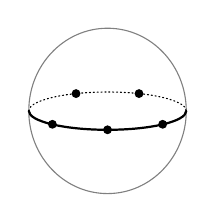
\begin{tikzpicture}[x=1cm,y=1cm,line cap=round,line join=round]\draw[gray] (0,0) ellipse (1 and 1.05);\draw[thick] (-1,0) arc[start angle=180,end angle=360,x radius=1,y radius=.24];\draw[densely dotted] (-1,0) arc[start angle=180,end angle=0,x radius=1,y radius=.24];\fill (-0.7,-0.17) circle(1.6pt);\fill (0,-0.24) circle(1.6pt);\fill (0.7,-0.17) circle(1.6pt);\fill (-0.4,0.22) circle(1.6pt);\fill (0.4,0.22) circle(1.6pt);\end{tikzpicture}}}
\sbox{181}{\figure{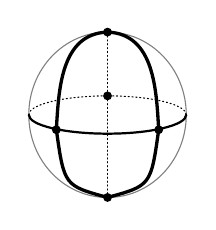
\begin{tikzpicture}[x=1cm,y=1cm,line cap=round,line join=round]\draw[gray] (0,0) ellipse (1 and 1.05);\draw[thick] (-1,0) arc[start angle=180,end angle=360,x radius=1,y radius=.24];\draw[densely dotted] (-1,0) arc[start angle=180,end angle=0,x radius=1,y radius=.24];\draw[very thick] (0,1.05) .. controls (-.6,1.03) and (-.62,.3) .. (-.65,-.19);\draw[very thick] (0,1.05) .. controls (.6,1.03) and (.62,.3) .. (.65,-.19);\draw[densely dotted] (0,1.05)--(0,.24);\draw[very thick] (-.65,-.19) .. controls (-.55,-.9) .. (0,-1.05) .. controls (.55,-.9) .. (.65,-.19);\draw[densely dotted] (0,.24)--(0,-1.05);\fill (0,1.05) circle(1.6pt);\fill (-0.65,-0.19) circle(1.6pt);\fill (0.65,-0.19) circle(1.6pt);\fill (0,0.24) circle(1.6pt);\fill (0,-1.05) circle(1.6pt);\end{tikzpicture}}}
\sbox{182}{\figure{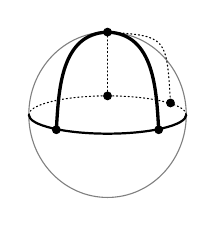
\begin{tikzpicture}[x=1cm,y=1cm,line cap=round,line join=round]\draw[gray] (0,0) ellipse (1 and 1.05);\draw[thick] (-1,0) arc[start angle=180,end angle=360,x radius=1,y radius=.24];\draw[densely dotted] (-1,0) arc[start angle=180,end angle=0,x radius=1,y radius=.24];\draw[very thick] (0,1.05) .. controls (-.6,1.03) and (-.62,.3) .. (-.65,-.19);\draw[very thick] (0,1.05) .. controls (.6,1.03) and (.62,.3) .. (.65,-.19);\draw[densely dotted] (0,1.05)--(0,.24);\draw[densely dotted] (0,1.05) .. controls (.75,1) .. (.8,.15);\fill (0,1.05) circle(1.6pt);\fill (-0.65,-0.19) circle(1.6pt);\fill (0.65,-0.19) circle(1.6pt);\fill (0,0.24) circle(1.6pt);\fill (0.8,0.15) circle(1.6pt);\end{tikzpicture}}}
\sbox{183}{\figure{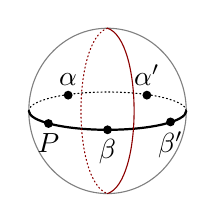
\begin{tikzpicture}[x=1cm,y=1cm,line cap=round,line join=round]\draw[gray] (0,0) ellipse (1 and 1.05);\draw[thick] (-1,0) arc[start angle=180,end angle=360,x radius=1,y radius=.24];\draw[densely dotted] (-1,0) arc[start angle=180,end angle=0,x radius=1,y radius=.24];\draw[red!55!black] (0,1.05) .. controls (.45,.9) and (.45,-.9) .. (0,-1.05);\draw[red!55!black,densely dotted] (0,1.05) .. controls (-.45,.9) and (-.45,-.9) .. (0,-1.05);\fill (-0.5,0.2) circle(1.6pt) node[above] {$\alpha$};\fill (0.5,0.2) circle(1.6pt) node[above] {$\alpha'$};\fill (-0.75,-0.16) circle(1.6pt) node[below] {$P$};\fill (0,-0.24) circle(1.6pt) node[below] {$\beta$};\fill (0.8,-0.14) circle(1.6pt) node[below] {$\beta'$};\end{tikzpicture}}}
\sbox{184}{\figure{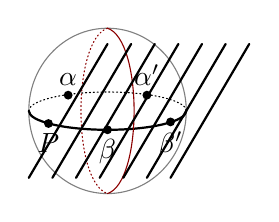
\begin{tikzpicture}[x=1cm,y=1cm,line cap=round,line join=round]\draw[gray] (0,0) ellipse (1 and 1.05);\draw[thick] (-1,0) arc[start angle=180,end angle=360,x radius=1,y radius=.24];\draw[densely dotted] (-1,0) arc[start angle=180,end angle=0,x radius=1,y radius=.24];\draw[red!55!black] (0,1.05) .. controls (.45,.9) and (.45,-.9) .. (0,-1.05);\draw[red!55!black,densely dotted] (0,1.05) .. controls (-.45,.9) and (-.45,-.9) .. (0,-1.05);\fill (-0.5,0.2) circle(1.6pt) node[above] {$\alpha$};\fill (0.5,0.2) circle(1.6pt) node[above] {$\alpha'$};\fill (-0.75,-0.16) circle(1.6pt) node[below] {$P$};\fill (0,-0.24) circle(1.6pt) node[below] {$\beta$};\fill (0.8,-0.14) circle(1.6pt) node[below] {$\beta'$};\draw[thick] (-1,-.85)--(0,.85);\draw[thick] (-0.7,-.85)--(0.30000000000000004,.85);\draw[thick] (-0.4,-.85)--(0.6,.85);\draw[thick] (-0.1,-.85)--(0.9,.85);\draw[thick] (0.2,-.85)--(1.2,.85);\draw[thick] (0.5,-.85)--(1.5,.85);\draw[thick] (0.8,-.85)--(1.8,.85);\end{tikzpicture}}}
\sbox{185}{\figure{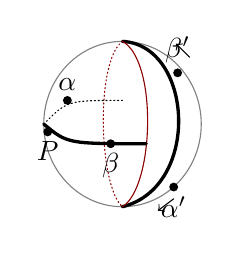
\begin{tikzpicture}[x=1cm,y=1cm,line cap=round,line join=round]\draw[gray] (0,0) ellipse (1 and 1.05);\draw[very thick] (0,1.05) .. controls (.9,1) and (1,-.8) .. (0,-1.05);\draw[red!55!black] (0,1.05) .. controls (.45,.8) and (.4,-.8) .. (0,-1.05);\draw[red!55!black,densely dotted] (0,1.05) .. controls (-.35,.8) and (-.3,-.8) .. (0,-1.05);\draw[very thick] (-1,0)..controls(-.7,-.25)..(.3,-.25);\draw[densely dotted] (-1,0)..controls(-.7,.3)..(0,.3);\fill (-0.7,0.3) circle(1.6pt) node[above] {$\alpha$};\fill (0.7,0.65) circle(1.6pt) node[above] {$\beta'$};\fill (-0.95,-0.1) circle(1.6pt) node[below] {$P$};\fill (-0.15,-0.25) circle(1.6pt) node[below] {$\beta$};\fill (0.65,-0.8) circle(1.6pt) node[below] {$\alpha'$};\draw[->] (.85,.85)--(.68,1.02);\draw[->] (.65,-.95)--(.45,-1.1);\end{tikzpicture}}}
\sbox{186}{\figure{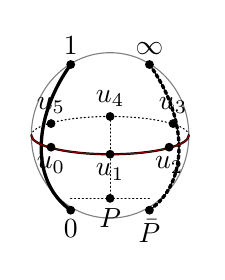
\begin{tikzpicture}[x=1cm,y=1cm,line cap=round,line join=round]\draw[gray] (0,0) ellipse (1 and 1.05);\draw[thick] (-1,0) arc[start angle=180,end angle=360,x radius=1,y radius=.24];\draw[densely dotted] (-1,0) arc[start angle=180,end angle=0,x radius=1,y radius=.24];\draw[very thick] (-.5,.9)..controls(-1,.2)and(-1,-.6)..(-.5,-.95);\draw[very thick,densely dotted] (.5,.9)..controls(1,.2)and(1,-.6)..(.5,-.95);\draw[red!55!black] (-1,0) arc[start angle=180,end angle=360,x radius=1,y radius=.24];\draw[densely dotted] (-.5,-.8)--(.5,-.8);\draw[densely dotted] (0,.24)--(0,-.8);\fill (-0.5,0.9) circle(1.6pt) node[above] {$1$};\fill (0.5,0.9) circle(1.6pt) node[above] {$\infty$};\fill (-0.5,-0.95) circle(1.6pt) node[below] {$0$};\fill (0.5,-0.95) circle(1.6pt) node[below] {$\bar P$};\fill (0,-0.8) circle(1.6pt) node[below] {$P$};\fill (-0.75,-0.15) circle(1.6pt) node[below] {$u_0$};\fill (0,-0.24) circle(1.6pt) node[below] {$u_1$};\fill (0.75,-0.15) circle(1.6pt) node[below] {$u_2$};\fill (0.8,0.15) circle(1.6pt) node[above] {$u_3$};\fill (0,0.24) circle(1.6pt) node[above] {$u_4$};\fill (-0.75,0.15) circle(1.6pt) node[above] {$u_5$};\end{tikzpicture}}}
\sbox{187}{\figure{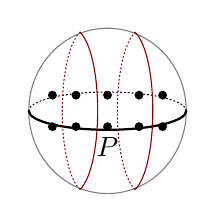
\begin{tikzpicture}[x=1cm,y=1cm,line cap=round,line join=round]\draw[gray] (0,0) ellipse (1 and 1.05);\draw[thick] (-1,0) arc[start angle=180,end angle=360,x radius=1,y radius=.24];\draw[densely dotted] (-1,0) arc[start angle=180,end angle=0,x radius=1,y radius=.24];\draw[red!55!black] (-0.35,1) .. controls (-0.04999999999999999,.7) and (-0.04999999999999999,-.7) .. (-0.35,-1);\draw[red!55!black,densely dotted] (-0.35,1) .. controls (-0.6499999999999999,.7) and (-0.6499999999999999,-.7) .. (-0.35,-1);\draw[red!55!black] (0.35,1) .. controls (0.6499999999999999,.7) and (0.6499999999999999,-.7) .. (0.35,-1);\draw[red!55!black,densely dotted] (0.35,1) .. controls (0.04999999999999999,.7) and (0.04999999999999999,-.7) .. (0.35,-1);\fill (-0.7,-0.2) circle(1.6pt);\fill (-0.7,0.2) circle(1.6pt);\fill (-0.4,-0.2) circle(1.6pt);\fill (-0.4,0.2) circle(1.6pt);\fill (0,-0.2) circle(1.6pt);\fill (0,0.2) circle(1.6pt);\fill (0.4,-0.2) circle(1.6pt);\fill (0.4,0.2) circle(1.6pt);\fill (0.7,-0.2) circle(1.6pt);\fill (0.7,0.2) circle(1.6pt);\node[below] at (0,-.22) {$P$};\end{tikzpicture}}}
\sbox{188}{\figure{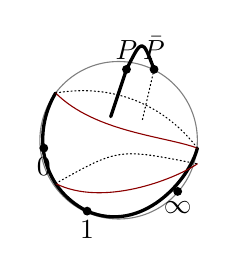
\begin{tikzpicture}[x=1cm,y=1cm,line cap=round,line join=round]\draw[gray] (0,0) circle(1);\draw[very thick] (-.8,.6)..controls(-1.1,.1)and(-1,-.6)..(-.4,-.9)..controls(.3,-1.2)and(.9,-.5)..(1,-.1);\draw[red!55!black] (-.8,.6)..controls(-.3,.1)and(.6,.05)..(1,-.1);\draw[densely dotted] (-.8,.6)..controls(.1,.75)and(.7,.3)..(1,-.1);\draw[red!55!black] (-.8,-.55)..controls(-.2,-.85)and(.7,-.5)..(1,-.3);\draw[densely dotted] (-.8,-.55)..controls(0,-.1)..(1,-.3);\draw[very thick] (-.1,.3)--(.1,.9)..controls(.3,1.3)..(.45,.9);\draw[densely dotted] (.45,.9)--(.3,.25);\fill (-0.95,-0.1) circle(1.6pt) node[below] {$0$};\fill (-0.4,-0.9) circle(1.6pt) node[below] {$1$};\fill (0.75,-0.65) circle(1.6pt) node[below] {$\infty$};\fill (0.1,0.9) circle(1.6pt) node[above] {$P$};\fill (0.45,0.9) circle(1.6pt) node[above] {$\bar P$};\end{tikzpicture}}}
\sbox{189}{\figure{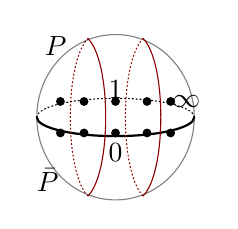
\begin{tikzpicture}[x=1cm,y=1cm,line cap=round,line join=round]\draw[gray] (0,0) ellipse (1 and 1.05);\draw[thick] (-1,0) arc[start angle=180,end angle=360,x radius=1,y radius=.24];\draw[densely dotted] (-1,0) arc[start angle=180,end angle=0,x radius=1,y radius=.24];\draw[red!55!black] (-0.35,1) .. controls (-0.04999999999999999,.7) and (-0.04999999999999999,-.7) .. (-0.35,-1);\draw[red!55!black,densely dotted] (-0.35,1) .. controls (-0.6499999999999999,.7) and (-0.6499999999999999,-.7) .. (-0.35,-1);\draw[red!55!black] (0.35,1) .. controls (0.6499999999999999,.7) and (0.6499999999999999,-.7) .. (0.35,-1);\draw[red!55!black,densely dotted] (0.35,1) .. controls (0.04999999999999999,.7) and (0.04999999999999999,-.7) .. (0.35,-1);\fill (-0.7,-0.2) circle(1.6pt);\fill (-0.7,0.2) circle(1.6pt);\fill (-0.4,-0.2) circle(1.6pt);\fill (-0.4,0.2) circle(1.6pt);\fill (0,-0.2) circle(1.6pt);\fill (0,0.2) circle(1.6pt);\fill (0.4,-0.2) circle(1.6pt);\fill (0.4,0.2) circle(1.6pt);\fill (0.7,-0.2) circle(1.6pt);\fill (0.7,0.2) circle(1.6pt);\node[left] at (-.5,.9) {$P$};\node[left] at (-.6,-.8) {$\bar P$};\node[right] at (.6,.2) {$\infty$};\node at (0,.35) {$1$};\node at (0,-.45) {$0$};\end{tikzpicture}}}
\sbox{190}{\figure{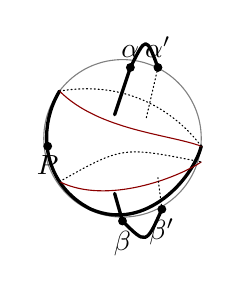
\begin{tikzpicture}[x=1cm,y=1cm,line cap=round,line join=round]\draw[gray] (0,0) circle(1);\draw[very thick] (-.8,.6)..controls(-1.1,.1)and(-1,-.6)..(-.4,-.9)..controls(.3,-1.2)and(.9,-.5)..(1,-.1);\draw[red!55!black] (-.8,.6)..controls(-.3,.1)and(.6,.05)..(1,-.1);\draw[densely dotted] (-.8,.6)..controls(.1,.75)and(.7,.3)..(1,-.1);\draw[red!55!black] (-.8,-.55)..controls(-.2,-.85)and(.7,-.5)..(1,-.3);\draw[densely dotted] (-.8,-.55)..controls(0,-.1)..(1,-.3);\draw[very thick] (-.1,.3)--(.1,.9)..controls(.3,1.3)..(.45,.9);\draw[densely dotted] (.45,.9)--(.3,.25);\draw[very thick] (-.1,-.7)--(0,-1.05)..controls(.3,-1.35)..(.5,-.9);\draw[densely dotted] (.5,-.9)--(.45,-.5);\fill (-0.95,-0.1) circle(1.6pt) node[below] {$P$};\fill (0.1,0.9) circle(1.6pt) node[above] {$\alpha$};\fill (0.45,0.9) circle(1.6pt) node[above] {$\alpha'$};\fill (0,-1.05) circle(1.6pt) node[below] {$\beta$};\fill (0.5,-0.9) circle(1.6pt) node[below] {$\beta'$};\end{tikzpicture}}}
\sbox{191}{\figure{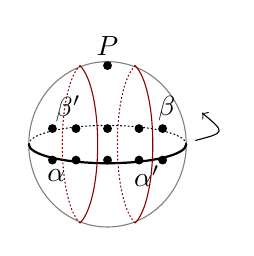
\begin{tikzpicture}[x=1cm,y=1cm,line cap=round,line join=round]\draw[gray] (0,0) ellipse (1 and 1.05);\draw[thick] (-1,0) arc[start angle=180,end angle=360,x radius=1,y radius=.24];\draw[densely dotted] (-1,0) arc[start angle=180,end angle=0,x radius=1,y radius=.24];\draw[red!55!black] (-0.35,1) .. controls (-0.04999999999999999,.7) and (-0.04999999999999999,-.7) .. (-0.35,-1);\draw[red!55!black,densely dotted] (-0.35,1) .. controls (-0.6499999999999999,.7) and (-0.6499999999999999,-.7) .. (-0.35,-1);\draw[red!55!black] (0.35,1) .. controls (0.6499999999999999,.7) and (0.6499999999999999,-.7) .. (0.35,-1);\draw[red!55!black,densely dotted] (0.35,1) .. controls (0.04999999999999999,.7) and (0.04999999999999999,-.7) .. (0.35,-1);\fill (-0.7,-0.2) circle(1.6pt);\fill (-0.7,0.2) circle(1.6pt);\fill (-0.4,-0.2) circle(1.6pt);\fill (-0.4,0.2) circle(1.6pt);\fill (0,-0.2) circle(1.6pt);\fill (0,0.2) circle(1.6pt);\fill (0.4,-0.2) circle(1.6pt);\fill (0.4,0.2) circle(1.6pt);\fill (0.7,-0.2) circle(1.6pt);\fill (0.7,0.2) circle(1.6pt);\fill (0,1) circle(1.6pt) node[above] {$P$};\node at (-.65,-.4) {$\alpha$};\node at (.5,-.4) {$\alpha^\prime$};\node at (-.5,.45) {$\beta^\prime$};\node at (.75,.45) {$\beta$};\draw[->] (1.12,.05)..controls(1.5,.15)..(1.2,.4);\end{tikzpicture}}}
\diagram{\begin{tikzcd}[ampersand replacement=\&,column sep=9em,row sep=10em]
\begin{gathered}\mathrm{I}_{10}\ (\text{pentagonale})\\
\figure{\usebox{180}}\\
\text{12 structures pentagonales sur }K\\
\{\sigma,\sigma^{-1}\}\in P_2\unsure{\mathrm{Circ}}(K)\\
G\simeq\mathbb D_5\\
\widetilde G\simeq\mathbb D_5\times\{1,\sigma\}\end{gathered}\&\begin{gathered}\mathrm I_6\ (\text{bitétraédrale})\\
\figure{\usebox{181}}\\
\text{20 structures }K=J\amalg\omega\\
\text{avec }\omega\xrightarrow{\sim}\underline\omega(J)\\
G\simeq\unsure{\mathfrak S}_J\simeq\unsure{\mathfrak S}_3\\
\widetilde G\simeq\unsure{\mathfrak S}_3\times\{1,\sigma\}\end{gathered} \arrow[r,"{3\quad f_{B,s}\quad2}","{(B\in\mathrm{Bit\acute et}(K),\ s\in\pi(B)=J)}"'] \& \begin{gathered}\mathrm I_4\ (\text{pyramidale})\\
\figure{\usebox{182}}\\
\text{30 structures carrés orientés}\\
K\simeq\{P\}\amalg I\\
I\ \text{structure carré \uline{orienté}}\ (Q,\omega)=\vec Q\\
I=\coprod_{\alpha\in\delta}\alpha\qquad\delta=\text{ens. des diagonales }\alpha\\
\omega\in\delta\wedge\bigwedge_{\alpha\in\delta}\alpha\\
G=\widetilde G=\mathbb Z/4\mathbb Z\end{gathered} \\
\begin{gathered}\mathrm{II}_2\ (\text{carré-triangle droit})\\
\figure{\usebox{183}}\\
\text{2 sommets-repères}\quad\deleted{\text{\unsure{repères}}}\\
\text{60 structures ``pentagone}\\
\text{avec sommet'' sur }K\\
\text{i.e. }K\simeq J\amalg\omega,\ \text{avec }\omega\hookrightarrow J\\
\text{i.e. }P\in J\text{ et }\omega\xrightarrow{\sim}\omega'=J\setminus\{P\}\\
G\simeq\mathbb Z/2\mathbb Z\\
\widetilde G\simeq\mathbb Z/2\mathbb Z\times\{1,\sigma\}\end{gathered} \arrow[u,"{1\quad\gamma_{\pi,s}\quad5}","{(\pi\in\mathrm{Pent}(K),\ s\in K)}"'] \arrow[r,"{1\quad\tau_{\pi,s}=\mathrm{tw}_{1/4}\quad1}"] \& \begin{gathered}\mathrm{II}'_2=\mathrm{Tw}_{1/4}\mathrm{II}_2\\
(\text{carré-triangle gauche})\\
\text{4 sommets}\ \deleted{\text{\unsure{repères}}}\\
\deleted{\figure{\usebox{184}}}\quad\figure{\usebox{185}}\\
\text{mêmes paramètres que }\mathrm{II}_2\\
G\simeq\mathbb Z/2\mathbb Z,\ \widetilde G\simeq\mathbb Z/2\mathbb Z\times\{1,\sigma\}\end{gathered} \arrow[u,"{\unsure{\gamma^1_{\pi,s}}\quad3}","{\text{comp. avec }\vec Q}"'] \arrow[ur,bend left=10,pos=.73,"{2\quad f_{\vec Q,\unsure{\omega},a}\quad4}","{(\vec Q\in\overrightarrow{\mathrm{Carr}}(K),\ a\in\unsure{\Lambda}(Q))}"'] \& \begin{gathered}\mathrm{II}_1\ (\text{tétraèdre-triangle})\\
\figure{\usebox{186}}\\
\text{6 sommets-repères}\\
\text{120 structures entièrement}\\
\text{épinglées,}\\
G=\deleted{\unsure{1}}=\{1\},\quad\widetilde G=\{1,\sigma\}\\
\left[\begin{gathered}K=J\amalg\varepsilon\quad\operatorname{card}J=3,\operatorname{card}\varepsilon=2\\\omega\in\underline\omega(J),\ r\in J\times\varepsilon\\\tau_r^0:\mathrm{II}_1(J,\varepsilon)\longrightarrow\mathrm{II}_1(u_\omega(r))\\\text{où }u_\omega=\omega\times(-1)\text{ sur }J\times\varepsilon\end{gathered}\right]\end{gathered} \arrow[ul,pos=.73,"{1\quad\gamma_r^0\quad6}","{\text{comp. avec }\vec Q;\ (\pi\in\mathrm{Pent}(K),s\in K)}"'] \arrow[loop right,"{\tau_r^0=\mathrm{tw}_{1/6}}"] \\
\begin{gathered}\mathrm{III}_2\ (\text{triple triangle droit})\\
\figure{\usebox{187}}\\
\text{2+2 sommets-repère}\\
\text{60 structures ``pentagone avec}\\
\text{sommet'' sur }K,\\
G=\mathbb Z/2\mathbb Z,\widetilde G\simeq\mathbb Z/2\mathbb Z\times\{1,\sigma\}\end{gathered} \arrow[u,"{2\quad\gamma_{\pi,\rho}\quad2}","{(\pi\in\mathrm{Pent}(K),\rho\in\mathrm{Rep}\,\pi)}"'] \arrow[r,"{2\quad\tau_{\pi,\rho}=\mathrm{tw}_{1/3}\quad1}"] \& \begin{gathered}\mathrm{III}_1\ (\text{triple triangle sem.-gauche})\\
\figure{\usebox{188}}\quad=\quad\figure{\usebox{189}}\\
\text{2+4 sommets-repère}\\
\text{120 structures épinglées}\\
G=1,\widetilde G=\{1,\sigma\}\end{gathered} \arrow[u,"{1\quad\gamma_r^1\quad2}"] \arrow[ur,"{3\quad\gamma_{\bar r}^1\quad3}","{(r\in\mathrm{Rep}(K))}"'] \arrow[ul,bend left=30,"{\gamma_r^2\quad2}"] \arrow[r,"{1\quad\tau_r^1\quad2}"] \& \begin{gathered}\mathrm{III}'_2\ (\text{triple triangle gauche})\\
\figure{\usebox{190}}\quad\simeq\quad\figure{\usebox{191}}\\
\text{4+4 sommets-repère}\\
\text{60 structures de carré orienté à}\\
\text{codiagonales, }K=\{P\}\amalg I,\\
I\ \text{muni d’une \inserted{str.} carré en codiagonales }\unsure{\delta}=\{\alpha,\beta,\alpha',\beta'\}\\
\text{i.e. d’un repère de }\unsure{\mathfrak X}(I)\\
G=\mathbb Z/2\mathbb Z\deleted{\unsure{*}},\quad\widetilde G\simeq\mathbb Z/2\mathbb Z\times\mathbb Z/2\mathbb Z\simeq\mathbb Z/2\mathbb Z\times\{1,\sigma\}\end{gathered} \arrow[uu,bend right=70,"{1\quad\gamma_r^{21}\quad2}"]
\end{tikzcd}}

\diagram{\[\begin{array}{lll}
\uline{\text{niveau }2}&\mathrm I_{10},\mathrm I_6,\mathrm I_4&12+20+30=62\\
\uline{\text{niveau }1}&\mathrm{II}_2,\mathrm{II}'_2,\mathrm{II}_1&60+60+120=240\\
\uline{\text{niveau }0}&\mathrm{III}_2,\mathrm{III}_1,\mathrm{III}'_2&60+120+60=240\\
&&\underline{542}
\end{array}\]}

(l’indice indique l’ordre de \(G=\operatorname{Aut}^{+}\) ; donc le nb de structures est \(120/i\))

\uline{NB} Sauf \(\mathrm I_4\), toutes ces structures sont ``réelles''.

\[\begin{array}{ll}
\pi\in\mathrm{Pent}(K),&B\in\mathrm{Bit\acute et}(K)\\
s\in K,&\vec Q\in\overrightarrow{\mathrm{Carr}}(K)\\
\rho\in\mathrm{Rep}(\pi);&r\in\mathrm{Rep}(K)
\end{array}\]
(\uline{NB} \(\{(\pi,\rho)\}\simeq\mathrm{Rep}(K)\)).
\unsure{\texttt{GUTS OUTPUT FOR PREDONT DELIVER AT 0000 - PREDONT.MODULEF5}}

\unsure{\texttt{GUTS OUTPUT FOR PREDONT DELIVER AT 0000 - PREDONT.MODULEF5}}

\unsure{\texttt{GUTS OUTPUT FOR PREDONT DELIVER AT 0000 - PREDONT.MODULEF5}}

\unsure{\texttt{GUTS OUTPUT FOR PREDONT DELIVER AT 0000 - PREDONT.MODULEF5}}

\unsure{\texttt{GUTS OUTPUT FOR PREDONT DELIVER AT 0000 - PREDONT.MODULEF5}}

\unsure{\texttt{GUTS OUTPUT FOR PREDONT DELIVER AT 0000 - PREDONT.MODULEF5}}

\unsure{\texttt{GUTS OUTPUT FOR PREDONT DELIVER AT 0000 - PREDONT.MODULEF5}}

\unsure{\texttt{GUTS OUTPUT FOR PREDONT DELIVER AT 0000 - PREDONT.MODULEF5}}

\unsure{\texttt{GUTS OUTPUT FOR PREDONT DELIVER AT 0000 - PREDONT.MODULEF5}}

\unsure{\texttt{GUTS OUTPUT FOR PREDONT DELIVER AT 0000 - PREDONT.MODULEF5}}

\unsure{\texttt{GUTS OUTPUT FOR PREDONT DELIVER AT 0000 - PREDONT.MODULEF5}}

\unsure{\texttt{GUTS OUTPUT FOR PREDONT DELIVER AT 0000 - PREDONT.MODULEF5}}

\unsure{\texttt{GUTS OUTPUT FOR PREDONT DELIVER AT 0000 - PREDONT.MODULEF5}}

\unsure{\texttt{GUTS OUTPUT FOR PREDONT DELIVER AT 0000 - PREDONT.MODULEF5}}

\unsure{\texttt{GUTS OUTPUT FOR PREDONT DELIVER AT 0000 - PREDONT.MODULEF5}}

\unsure{\texttt{GUTS OUTPUT FOR PREDONT DELIVER AT 0000 - PREDONT.MODULEF5}}

\unsure{\texttt{GUTS OUTPUT FOR PREDONT DELIVER AT 0000 - PREDONT.MODULEF5}}

\unsure{\texttt{GUTS OUTPUT FOR PREDONT DELIVER AT 0000 - PREDONT.MODULEF5}}

\unsure{\texttt{GUTS OUTPUT FOR PREDONT DELIVER AT 0000 - PREDONT.MODULEF5}}

\unsure{\texttt{GUTS OUTPUT FOR PREDONT DELIVER AT 0000 - PREDONT.MODULEF5}}

\unsure{\texttt{GUTS OUTPUT FOR PREDONT DELIVER AT 0000 - PREDONT.MODULEF5}}

\unsure{\texttt{GUTS OUTPUT FOR PREDONT DELIVER AT 0000 - PREDONT.MODULEF5}}

\unsure{\texttt{GUTS OUTPUT FOR PREDONT DELIVER AT 0000 - PREDONT.MODULEF5}}

\unsure{\texttt{GUTS OUTPUT FOR PREDONT DELIVER AT 0000 - PREDONT.MODULEF5}}

\unsure{\texttt{GUTS OUTPUT FOR PREDONT DELIVER AT 0000 - PREDONT.MODULEF5}}

\unsure{\texttt{GUTS OUTPUT FOR PREDONT DELIVER AT 0000 - PREDONT.MODULEF5}}

\unsure{\texttt{GUTS OUTPUT FOR PREDONT DELIVER AT 0000 - PREDONT.MODULEF5}}

\unsure{\texttt{GUTS OUTPUT FOR PREDONT DELIVER AT 0000 - PREDONT.MODULEF5}}
\mspage{30}
\scanpage{32}
\figure{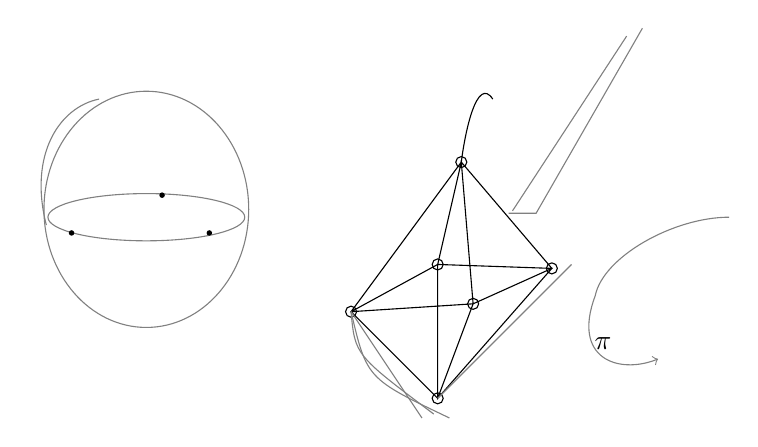
\begin{tikzpicture}[x=1cm,y=1cm]
\draw[gray] (0,0) ellipse (1.3 and 1.5);
\draw[gray] (-1.27,-.2)..controls(-1.5,.7)and(-1.1,1.3)..(-.6,1.4);
\draw[gray] (-1.25,-.1) arc[start angle=180,end angle=360,x radius=1.25,y radius=.3];
\draw[gray] (-1.25,-.1) arc[start angle=180,end angle=0,x radius=1.25,y radius=.3];
\fill (-.95,-.3) circle(1pt);\fill (.8,-.3) circle(1pt);\fill (.2,.18) circle(1pt);
\begin{scope}[shift={(4,-.5)}]
\coordinate (a) at (0,1.1);\coordinate (b) at (-1.4,-.8);\coordinate(c) at (.15,-.7);\coordinate(d) at (1.15,-.25);\coordinate(e) at (-.3,-.2);\coordinate(f) at (-.3,-1.9);
\draw (a)--(b)--(c)--(d)--(a)--(c)--(f)--(b)--(e)--(d)--(f)--(e)--(a);
\foreach \p in {a,b,c,d,e,f}{\draw (\p) circle(2pt);}
\draw (a)..controls(.05,1.5)and(.2,2.2)..(.4,1.9);
\draw[gray] (.6,.45)--(.95,.45)--(2.3,2.8);
\draw[gray] (.65,.48)--(2.1,2.7);
\draw[gray] (b)..controls(-1.35,-1.35)..(-.35,-2.1);
\draw[gray] (b)..controls(-1.2,-1.65)..(-.15,-2.15);
\draw[gray] (b)--(-.5,-2.15);
\draw[gray] (f)--(1.4,-.2);
\end{scope}
\draw[gray,->] (7.4,-.1)..controls(6.7,-.1)and(5.8,-.6)..(5.7,-1.1)..controls(5.4,-1.9)and(6,-2.1)..(6.5,-1.9);
\node at (5.8,-1.7) {$\unsure{\pi}$};
\end{tikzpicture}}
\texttt{GUTS OUTPUT FOR PREDONT DELIVER AT 0000 - PREDONT.MODULEF5}\\
\texttt{GUTS OUTPUT FOR PREDONT DELIVER AT 0000 - PREDONT.MODULEF5}\\
\texttt{GUTS OUTPUT FOR PREDONT DELIVER AT 0000 - PREDONT.MODULEF5}\\
\texttt{GUTS OUTPUT FOR PREDONT DELIVER AT 0000 - PREDONT.MODULEF5}\\
\texttt{GUTS OUTPUT FOR PREDONT DELIVER AT 0000 - PREDONT.MODULEF5}\\
\texttt{GUTS OUTPUT FOR PREDONT DELIVER AT 0000 - PREDONT.MODULEF5}\\
\texttt{GUTS OUTPUT FOR PREDONT DELIVER AT 0000 - PREDONT.MODULEF5}\\
\texttt{GUTS OUTPUT FOR PREDONT DELIVER AT 0000 - PREDONT.MODULEF5}\\
\texttt{GUTS OUTPUT FOR PREDONT DELIVER AT 0000 - PREDONT.MODULEF5}\\
\texttt{GUTS OUTPUT FOR PREDONT DELIVER AT 0000 - PREDONT.MODULEF5}\\
\texttt{GUTS OUTPUT FOR PREDONT DELIVER AT 0000 - PREDONT.MODULEF5}\\
\texttt{GUTS OUTPUT FOR PREDONT DELIVER AT 0000 - PREDONT.MODULEF5}\\
\texttt{GUTS OUTPUT FOR PREDONT DELIVER AT 0000 - PREDONT.MODULEF5}\\
\texttt{GUTS OUTPUT FOR PREDONT DELIVER AT 0000 - PREDONT.MODULEF5}\\
\texttt{GUTS OUTPUT FOR PREDONT DELIVER AT 0000 - PREDONT.MODULEF5}\\
\texttt{GUTS OUTPUT FOR PREDONT DELIVER AT 0000 - PREDONT.MODULEF5}\\
\texttt{GUTS OUTPUT FOR PREDONT DELIVER AT 0000 - PREDONT.MODULEF5}\\
\texttt{GUTS OUTPUT FOR PREDONT DELIVER AT 0000 - PREDONT.MODULEF5}\\
\texttt{GUTS OUTPUT FOR PREDONT DELIVER AT 0000 - PREDONT.MODULEF5}\\
\texttt{GUTS OUTPUT FOR PREDONT DELIVER AT 0000 - PREDONT.MODULEF5}\\
\texttt{GUTS OUTPUT FOR PREDONT DELIVER AT 0000 - PREDONT.MODULEF5}\\
\texttt{GUTS OUTPUT FOR PREDONT DELIVER AT 0000 - PREDONT.MODULEF5}\\
\texttt{GUTS OUTPUT FOR PREDONT DELIVER AT 0000 - PREDONT.MODULEF5}\\
\texttt{GUTS OUTPUT FOR PREDONT DELIVER AT 0000 - PREDONT.MODULEF5}\\
\texttt{GUTS OUTPUT FOR PREDONT DELIVER AT 0000 - PREDONT.MODULEF5}\\
\texttt{GUTS OUTPUT FOR PREDONT DELIVER AT 0000 - PREDONT.MODULEF5}\\
\texttt{GUTS OUTPUT FOR PREDONT DELIVER AT 0000 - PREDONT.MODULEF5}\\
\texttt{GUTS OUTPUT FOR PREDONT DELIVER AT 0000 - PREDONT.MODULEF5}\\
\texttt{GUTS OUTPUT FOR PREDONT DELIVER AT 0000 - PREDONT.MODULEF5}\\
\texttt{GUTS OUTPUT FOR PREDONT DELIVER AT 0000 - PREDONT.MODULEF5}\\
\texttt{GUTS OUTPUT FOR PREDONT DELIVER AT 0000 - PREDONT.MODULEF5}\\
\texttt{GUTS OUTPUT FOR PREDONT DELIVER AT 0000 - PREDONT.MODULEF5}\\
\mspage{31}
\scanpage{33}
\diagram{\[
\begin{array}{rll}
180\left\{\begin{array}{l}60=3\times20=2\times30\\120=4\times30=2\times60\end{array}\right.
&\begin{array}{l}f_{B,s}\\f_{\vec Q,a}\end{array}\\[1em]
420\left\{\begin{array}{l}
60=1\times60=\unsure{4|1}\times60\\
\inserted{120=1\times120=1\times120}\\
60=1\times60=5\times12\\
60=1\times60=3\times20\\
120=1\times120=6\times20
\end{array}\right.
&\begin{array}{l}\tau_{\pi,s}\\\inserted{\tau_r^0}\\\gamma_{\pi,s}\\\gamma''_{\pi,s}\\\gamma_r^0\end{array}\\[1em]
\begin{array}{r}1020\\\deleted{\unsure{900}}\end{array}
\left\{\begin{array}{l}
120=2\times60=1\times120\\
120=\unsure{2\times60}=2\times60\\
120=\unsure{1\times120}=2\times60\\
120=1\times120=2\times60\\
3\times120=\deleted{\unsure{2\times60=2\times60}}\inserted{3\times40=3\times40}\\
120=2\times60=2\times60\\
60=1\times60=2\times30
\end{array}\right.
&\left.\begin{array}{l}
\tau_{\pi,\rho}\\
\unsure{\gamma}_{\pi,\rho}\\
\unsure{\tau_r^1}\\
\gamma_r^1\\
\gamma_r^{1'}\\
\gamma_r^2\\
\gamma_r^{2'}
\end{array}\right\}\\[1em]
\begin{array}{r}\deleted{\unsure{1500}}\\\inserted{1620}\end{array}
=5\times60+\unsure{11}\times120
\end{array}
\]}
\[
\tau=\text{``twist''}\qquad
\gamma=\text{``gommage''}
\]

Programme de travail :

1) déterminer un syst. fondamental de relations entre les \(1620\) flèches du diagramme, \unsure{se partageant} \deleted{entre} \(14\) \deleted{\unsure{orbites}} sous \(\unsure{\mathfrak S}_K\) (aux \(542\) sommets, se partageant entre \(9\) orbites)

\margin{en particulier, écrire toutes les flèches comme composés de flèches ``provenant de la dimension relative \(\leq1\)''}

\deleted{\unsure{2) Réduire}}

2) Reprendre la question, en éliminant les sommets du niveau \(0\) (sauf \unsure{peut-on} ceux de type \(\unsure{\mathrm I_{20}|\mathrm{III}_2}\) ?),
\deleted{et \(\mathrm{II}_1\) (\unsure{qui se déduit par} \(\mathrm{II}_1\) (qui revient \unsure{à ceux} du type \(\mathrm{III}_1\).) --- mais Attention au twist \inserted{\(\mathrm{tw}_{1/6}\)} \unsure{relativement} : \(\mathrm{II}_1\) (\unsure{qui donne un Autom. du même type}))}

3) Eliminer de plus les pièces \deleted{\unsure{gauches}} ``tétraédrales'' \(\mathrm{II}_1\) --- et toutes les pièces qui ne semblent pas simplifier la présentation des relations.

\figure{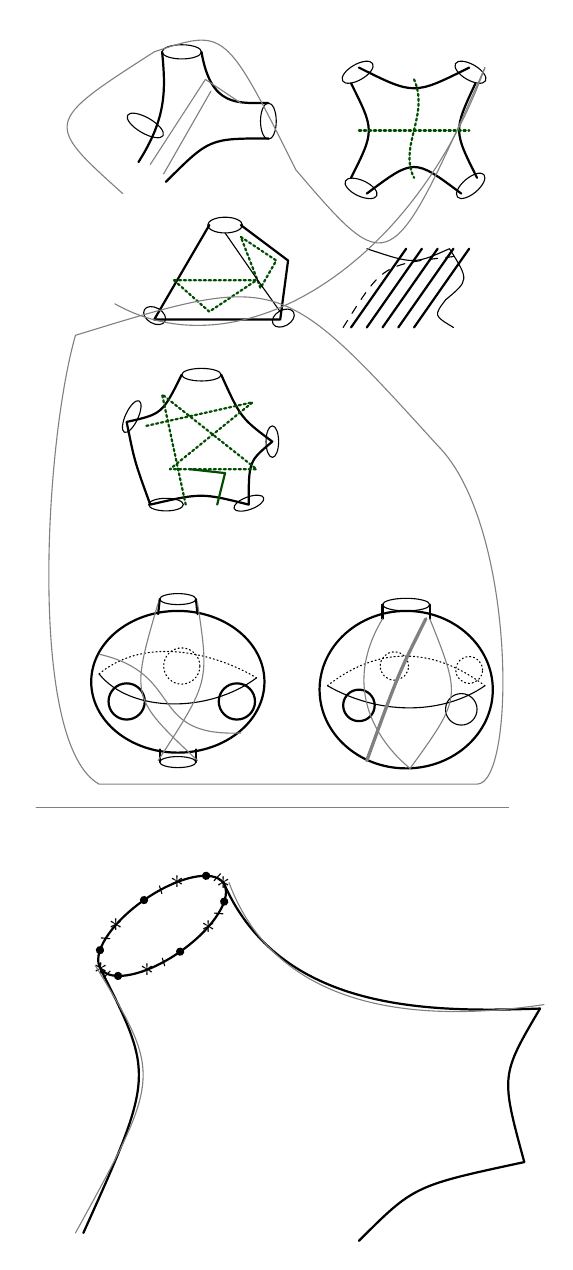
\begin{tikzpicture}[x=1cm,y=1cm,line cap=round,line join=round]
\begin{scope}[shift={(0,5)}]
\draw[thick] (-.5,1)..controls(-.45,.5)and(-.45,.15)..(-.8,-.4);
\draw[thick] (0,1)..controls(.12,.3)and(.45,.35)..(.85,.35);
\draw[thick] (.85,-.1)..controls(.1,-.1)..(-.45,-.65);
\draw (-.25,1) ellipse(.25 and .09);\draw[rotate=-30] (-.65,-.3) ellipse(.26 and .1);
\draw (.85,.12) ellipse(.1 and .23);
\draw[gray] (-.65,-.43)--(.05,.65)--(.5,.35);
\draw[gray] (-.48,-.55)--(.12,.5);
\end{scope}
\begin{scope}[shift={(2.7,5)}]
\draw[thick] (-.7,.8)..controls(0,.45)..(.7,.8);
\draw[thick] (.78,.6)..controls(.5,0)..(.8,-.6);
\draw[thick] (.6,-.8)..controls(0,-.35)..(-.6,-.8);
\draw[thick] (-.8,-.6)..controls(-.5,0)..(-.8,.6);
\draw[rotate=30](-.25,1)ellipse(.22 and .1);\draw[rotate=-30](.25,1)ellipse(.22 and .1);
\draw[rotate=-25](-.3,-.95)ellipse(.22 and .1);\draw[rotate=40](.1,-1)ellipse(.22 and .1);
\draw[green!30!black,densely dotted,thick] (-.7,0)--(.7,0);\draw[green!30!black,densely dotted,thick](0,.65)..controls(.2,.2)and(-.2,-.2)..(0,-.6);
\end{scope}
\begin{scope}[shift={(.3,3)}]
\draw[thick](-.2,.8)--(-.9,-.4)--(.7,-.4)--(.8,.35)--(.2,.8);
\draw (0,.8) ellipse(.22 and .1);\draw[rotate=-30](-.6,-.75)ellipse(.15 and .1);\draw[rotate=30](.45,-.7)ellipse(.15 and .1);
\draw[green!30!black,densely dotted,thick](-.65,.1)--(.4,.1)--(-.2,-.3)--(-.65,.1);
\draw[green!30!black,densely dotted,thick](.2,.65)--(.65,.35)--(.45,0)--(.2,.65);
\draw (0,.7)--(.45,.05)--(.7,-.3);
\end{scope}
\begin{scope}[shift={(2.5,3)}]
\draw[dashed](-.7,-.5)..controls(-.2,.3)..(.7,.4);
\draw(-.4,.5)..controls(.2,.3)..(.65,.5)..controls(.9,.1)..(.6,-.15)..controls(.45,-.35)..(.7,-.5);
\foreach \x in {-.6,-.4,-.2,0,.2}{\draw[thick](\x,-.5)--(\x+.7,.5);}
\end{scope}
\begin{scope}[shift={(0,.9)}]
\draw[thick](-.25,1)..controls(-.5,.5)..(-.95,.4)..controls(-.85,-.1)..(-.65,-.65)..controls(0,-.5)..(.6,-.65)..controls(.6,-.1)..(.9,.15)..controls(.5,.45)..(.25,1);
\draw(0,1)ellipse(.25 and .08);\draw[rotate=-25](-1,.05)ellipse(.08 and .22);\draw(.9,.15)ellipse(.08 and .2);
\draw(-.45,-.65)ellipse(.22 and .08);\draw[rotate=20](.35,-.8)ellipse(.2 and .08);
\draw[green!30!black,densely dotted,thick](-.7,.35)--(.65,.65)--(-.4,-.2)--(.7,-.2)--(-.5,.75)--(-.2,-.65);
\draw[green!30!black,thick](-.15,-.2)--(.3,-.25)--(.2,-.65);
\end{scope}
\begin{scope}[shift={(-.3,-2)}]
\draw[thick](0,0)ellipse(1.1 and .9);
\draw[thick](-.25,.86)--(-.23,1.05);\draw[thick](.25,.86)--(.23,1.05);\draw(0,1.05)ellipse(.23 and .07);
\draw[thick](-.23,-.86)--(-.23,-1.02);\draw[thick](.23,-.86)--(.23,-1.02);\draw(0,-1.02)ellipse(.23 and .07);
\draw[thick](-.65,-.25)circle(.23);\draw[thick](.75,-.25)circle(.23);\draw[densely dotted](.05,.2)circle(.23);
\draw(-1,.1)..controls(-.6,-.4)and(.4,-.4)..(1,.05);
\draw[densely dotted](-1,.1)..controls(-.4,.6)and(.5,.35)..(1,.05);
\draw[gray](-.25,1)..controls(-.6,-.2)..(.25,-1);\draw[gray](.25,1)..controls(.4,0)..(-.25,-1);
\draw[gray](-1,.35)..controls(.1,.1)and(-.4,-.7)..(.8,-.65);
\end{scope}
\begin{scope}[shift={(2.6,-2.1)}]
\draw[thick](0,0)ellipse(1.1 and 1);
\draw[thick](-.3,.9)--(-.3,1.08);\draw[thick](.3,.9)--(.3,1.08);\draw(0,1.08)ellipse(.3 and .08);
\draw[thick](-.6,-.2)circle(.2);\draw(.7,-.25)circle(.2);\draw[densely dotted](-.15,.3)circle(.18);\draw[densely dotted](.8,.25)circle(.17);
\draw(-1,.05)..controls(-.3,-.35)and(.5,-.3)..(1,.05);
\draw[densely dotted](-1,.05)..controls(-.3,.6)and(.4,.5)..(1,.05);
\draw[gray,very thick](.25,.9)..controls(-.1,.2)..(-.5,-.9);
\draw[gray](-.3,.9)..controls(-.9,-.1)and(-.2,-.8)..(.05,-1);
\draw[gray](.3,.9)..controls(.7,-.1)..(.05,-1);
\end{scope}
\draw[gray](-1.6,2.4)..controls(-2,1)and(-2.2,-2.8)..(-1.3,-3.3)--(3.5,-3.3)..controls(4,-3.3)and(4,0)..(3,1);
\draw[gray](-1.6,2.4)..controls(1,3.2)..(3,1);
\draw[gray](-1,4.2)..controls(-2,5.1)..(-.6,6)..controls(.3,6.3)..(1.2,4.5)..controls(2.4,3.1)..(3.6,5.8);
\draw[gray](-1.1,2.8)..controls(.5,1.9)and(2.7,3.3)..(3.6,5.8);
\draw[gray](-2.1,-3.6)--(3.9,-3.6);
\begin{scope}[shift={(-.5,-5.1)},rotate=35]
\draw[thick](0,0)ellipse(.95 and .4);
\foreach \a in {0,60,120,180,240,300}{\node at ({.95*cos(\a)},{.4*sin(\a)}) {$*$};}
\foreach \a in {30,90,150,210,270,330}{\fill ({.95*cos(\a)},{.4*sin(\a)})circle(1.5pt);}
\foreach \a in {15,75,135,195,255,315}{\draw ({.9*cos(\a)},{.35*sin(\a)})--({1.02*cos(\a)},{.45*sin(\a)});}
\end{scope}
\draw[thick](-1.28,-5.65)..controls(-.6,-7)..(-1.5,-9);
\draw[thick](.28,-4.55)..controls(1,-6.2)and(2.9,-6.2)..(4.3,-6.15);
\draw[thick](4.3,-6.15)..controls(3.8,-7)..(4.1,-8.1);
\draw[thick](4.1,-8.1)..controls(2.7,-8.4)..(2,-9.1);
\draw[gray](-1.35,-5.6)..controls(-.5,-7)..(-1.6,-9);
\draw[gray](.35,-4.55)..controls(1,-6.3)and(3,-6.3)..(4.35,-6.1);
\end{tikzpicture}}

\unsure{\texttt{//}}\illegible{6}

\unsure{\texttt{//}}\illegible{4}\unsure{\texttt{DISP=}}\illegible{2}

\unsure{\texttt{//}}\illegible{3}\unsure{\texttt{SYSPRINT}}\illegible{2}

\unsure{\texttt{//}}\illegible{3}\unsure{\texttt{VOL=SER}}\illegible{2}

\unsure{\texttt{//PL1}}\ \unsure{\texttt{DD DSN=}}\illegible{4}

\unsure{\texttt{//}}\illegible{5}

\unsure{\texttt{//}}\illegible{5}

\unsure{\texttt{//}}\illegible{4}\unsure{\texttt{DISP=(OLD,DELETE)}}

\unsure{\texttt{//}}\illegible{3}\unsure{\texttt{SPACE=(CYL,}}\illegible{2}

\unsure{\texttt{//}}\illegible{4}

\unsure{\texttt{//}}\illegible{4}

\unsure{\texttt{//}}\illegible{3}\unsure{\texttt{DELETE}}

\unsure{\texttt{//}}\illegible{4}\unsure{\texttt{VOL=SER}}\illegible{2}

\unsure{\texttt{//}}\illegible{3}\unsure{\texttt{SPACE=(CYL,}}\illegible{2}

\unsure{\texttt{//}}\illegible{3}\unsure{\texttt{DCB=}}\illegible{2}

\unsure{\texttt{//}}\illegible{3}\unsure{\texttt{DISP=(OLD,DELETE)}}

\unsure{\texttt{//}}\illegible{3}

\unsure{\texttt{//}}\illegible{4}

\unsure{\texttt{//}}\illegible{3}\unsure{\texttt{DCB=(RECFM=VBS,LRECL=20000,BLKSIZE=6440)}}

\unsure{\texttt{//}}\illegible{2}\unsure{\texttt{DISP=(CATLG),SPACE=(TRK,}}\illegible{2}

\unsure{\texttt{//}}\illegible{2}\unsure{\texttt{UNIT=SYSDA,VOL=SER=}}\illegible{1}

\unsure{\texttt{//}}\illegible{3}\unsure{\texttt{DCB=}}\illegible{2}

\unsure{\texttt{//}}\illegible{3}\unsure{\texttt{DISP=(MOD,DELETE)}}

\unsure{\texttt{//}}\illegible{2}\unsure{\texttt{DCB=(RECFM=VBS,LRECL=20000,BLKSIZE=6440)}}

\unsure{\texttt{//}}\illegible{2}\unsure{\texttt{UNIT=SYSDA,VOL=SER=}}\illegible{1}

\unsure{\texttt{//}}\illegible{2}\unsure{\texttt{DISP=(OLD,DELETE)}}

\unsure{\texttt{//}}\illegible{2}\unsure{\texttt{DSN=CHJ2.}}\illegible{1}

\unsure{\texttt{//}}\illegible{2}\unsure{\texttt{DISP=(OLD,DELETE)}}

\mspage{32}
\scanpage{34}
\mspage{1}
Systèmes spéciaux de cinq points sur une sphère complexe (plus gén.\textsuperscript{t} sur une \deleted{\unsure{courbe}} droite projective sur un corps alg clos \(k\) \unsure{de car. \(0\)})

Ce sont les systèmes \((\Sigma,I)\) où \(K\subset\Sigma\), \(\operatorname{card}K=5\), et tels qu’il existe un autom. non trivial de \((\Sigma,K)\) --- i.e. le groupe \inserted{\(G\)} des automorphismes de \((\Sigma,K)\) n’est pas réduit à \(1\). On fait la classification suivant la structure de ce groupe.

Soit \(g\in G\) d’ordre maximal. On peut identifier \(g\) à une permutation de \(I\), et la discussion se fait suivant la structure de celle-ci. Notons que \deleted{l’ordre de \(g\ne1\) est} tout autom. d’ordre fini de \(\Sigma\) \deleted{\(g\) d’ordre \(5\)} a exactement deux pts fixes, et que \deleted{\unsure{il est}} \inserted{si l’ordre est \(\nu\)}, \(\mathbb Z/\nu\mathbb Z\) opère librement sur \(\Sigma\setminus\Sigma^g\). Cela montre que
\[
K=K^g\amalg\text{orbites d’ordre }\nu,\quad\text{donc }2\leq\nu\leq5.
\]
\margin{l’opération est celle de \(\mu_\nu\) sur \(\mathbb G_m\).}

\textcircled{1} \(\nu=5\), alors \(K\) est une orbite --- OPS qui est l’orbite \(\mu_5(k)\) de \(\mu_5\) opérant sur \(\mathbb P^1_k\). Le groupe total des autom. est \(\mathbb D_5\). À isom. près, il y a un seul tel cas.

\margin{Structure pentagonale sur \(I\) (``pentagone'')}
\figure{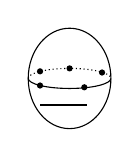
\begin{tikzpicture}[scale=.75]
\draw (0,0) ellipse(.7 and .85);
\draw (-.7,0) arc[start angle=180,end angle=360,x radius=.7,y radius=.17];
\draw[densely dotted] (-.7,0) arc[start angle=180,end angle=0,x radius=.7,y radius=.17];
\foreach \x/\y in {-.5/-.12,.25/-.15,.55/.1,-.5/.12,0/.17}{\fill(\x,\y)circle(1.5pt);}
\draw(-.5,-.45)--(.3,-.45);
\end{tikzpicture}}

\textcircled{2} \(\nu=4\) alors \deleted{\(\unsure{K^g}=\operatorname{card}I^g=1\)} \inserted{\(K^g=\{P\}\)}, et \(I\setminus\{P\}\) est une orbite. OPS que c’est \(\mu_4\), sur lequel \(\mu_4\) opère, et \(P\) est un pôle : \(\infty\). Le groupe total des autom. est \(\mathbb Z/4\mathbb Z\simeq\mu_4(k)\).

La catégorie de ces configurations est équivalente à celle des carrés orientés.

\margin{``pyramide carrée''}
\figure{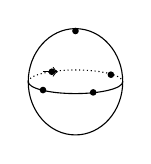
\begin{tikzpicture}[scale=.75]
\draw(0,0)ellipse(.8 and .9);
\draw(-.8,0)arc[start angle=180,end angle=360,x radius=.8,y radius=.2];
\draw[densely dotted](-.8,0)arc[start angle=180,end angle=0,x radius=.8,y radius=.2];
\foreach \x/\y in {0/.86,-.55/-.14,.3/-.18,.6/.12,-.4/.17}{\fill(\x,\y)circle(1.6pt);}
\draw[->](-.55,.17)--(-.3,.17);
\end{tikzpicture}}

\textcircled{3} \(\nu=3\), Alors \deleted{\(\unsure{K}\)} \(\operatorname{card}K^g=2\), \inserted{donc \(K^g=\Sigma^g\)}, et \(I\setminus K^g\) \inserted{\(=J\)} une orbite,
\deleted{Le groupe total des}
qu’on peut \unsure{supposer} \(\mu_3\). La catégorie de ces configurations est équivalente à celle des triangles combinatoires i.e. celle \(\mathrm{Ens}(3)\) des ens \(J\) de card \(3\).

À \(J\) on associe \(\Sigma_J\deleted{\unsure{\Sigma}}\) avec \(J\cup P_J\) (\(P_J\subset\Sigma_J\) ens des deux pôles de \(\Sigma_J\) en corr. \(1\)-\(1\) avec l’ens \(\omega(J)\) des or. de \(J\), si \(k=\mathbb C\)). Groupe des autom. est \(\mathbb D_3\).

\margin{\unsure{Partition} \(2\) et \(3\) (par ordre de \unsure{cardinaux|valeurs} ou \unsure{symétries})}
\margin{``bitétraèdre''}
\figure{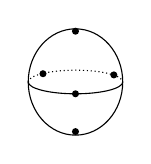
\begin{tikzpicture}[scale=.75]
\draw(0,0)ellipse(.8 and .9);
\draw(-.8,0)arc[start angle=180,end angle=360,x radius=.8,y radius=.2];
\draw[densely dotted](-.8,0)arc[start angle=180,end angle=0,x radius=.8,y radius=.2];
\foreach \x/\y in {0/.86,0/-.84,0/-.2,-.55/.14,.65/.12}{\fill(\x,\y)circle(1.7pt);}
\end{tikzpicture}}
\mspage{33}
\scanpage{35}
\mspage{2}
\textcircled{4} \(\nu=2\). \deleted{Il y a \unsure{deux cas}} \(K^g=\{P\}\), et \(K\setminus K^g\) \inserted{\(=I\)} est réunion de deux orbites. Ainsi, \(g\) est un autom. \deleted{\unsure{de}} ``universel'' de \(\Sigma\setminus I\) (\(g\in V(\unsure{D_I})\)) et \(P\) est \inserted{un de ses} pts fixes. \deleted{\unsure{De}} Cette fois, la situation a des ``modules'', p.ex. en choisissant une des deux orbites,

\deleted{OPS que l’opération de \(g\) sur elle est celle de \(\mu_2\) \inserted{\(=\{\pm1\}\)} sur \(\mu_2\) \inserted{\(=\{\pm1\}\)}, et \(P=0\), l’autre orbite est donnée par un \(\{t,-t\}\), avec \(\lambda=t^2\ne1,\lambda\in k^\times\) ---
donc \deleted{\(\lambda=\)} \(J=(0,\pm1,\pm\sqrt\lambda)\) \deleted{\(\unsure{\sqrt\lambda,\sqrt\lambda}\)}, avec \(\lambda\in\unsure{\mathbb P^1}(k)\setminus\{0,1,\infty\}\),
\unsure{en} \deleted{\unsure{changeant}} changeant le choix de l’orbite, on trouve
\[
(0,\pm1,\pm\sqrt{1/\lambda}).
\]
Prenons le paramètre \(\beta=\lambda+\frac1\lambda\), \inserted{\(\ne2\)}, donc \(\lambda^2-\beta\lambda+1=0\),
\deleted{\(\lambda=\frac12(\beta\pm\sqrt{\beta^2-4})\)},
on trouve \((0,\pm1,\pm\sqrt{\frac12(\beta\pm\sqrt{\beta^2-4})})\).
\unsure{Eliminer} \(0,\infty\), et \unsure{deux} \unsure{discriminant différent} \(2,\infty\) --- \unsure{comme} \deleted{\unsure{les}} \(\lambda\), et
\(g(z)=\frac{\lambda}{z}\), pts fixes.}

Cas moins intéressant que les précédents, de notre point de vue, car il y a des modules. Quand la structure \((\Sigma,I)\) est une structure carrée, on retrouve soit le cas \(2^\circ\) (si \(g\) laisse stables les deux diagonales), soit le cas d’un \inserted{des sommets} \deleted{\unsure{carré}} carré sphérique \unsure{équilatéral}, et du milieu de l’une des arêtes. \inserted{Est-ce le cas \(\unsure{1^\circ|2^\circ}\) ?} Quand c’est une structure tétraédrale, \(P\) est un des \inserted{\(6\)} sommets de l’octaèdre associé.

\figure{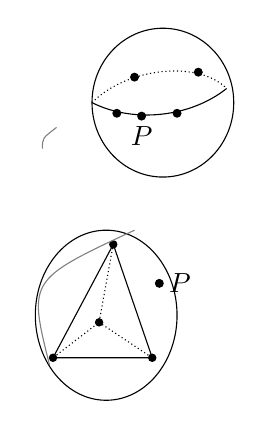
\begin{tikzpicture}[scale=.9]
\draw(0,0)ellipse(1 and 1.05);
\draw(-1,0)..controls(-.4,-.3)and(.4,-.2)..(.9,.2);
\draw[densely dotted](-1,0)..controls(-.5,.5)and(.5,.6)..(.9,.2);
\foreach \x/\y in {-.65/-.15,-.3/-.19,.2/-.15,-.4/.36,.5/.43}{\fill(\x,\y)circle(1.8pt);}
\node[below]at(-.3,-.2){$P$};
\draw[gray](-1.5,-.35)..controls(-1.7,-.5)..(-1.7,-.65);
\begin{scope}[shift={(-.8,-3)}]
\draw(0,0)ellipse(1 and 1.2);
\draw(-.75,-.6)--(.1,1)--(.65,-.6)--cycle;
\draw[densely dotted](.1,1)--(-.1,-.1)--(-.75,-.6);
\draw[densely dotted](-.1,-.1)--(.65,-.6);
\foreach \x/\y in {.1/1,-.75/-.6,.65/-.6,-.1/-.1}{\fill(\x,\y)circle(1.7pt);}
\fill(.75,.45)circle(1.8pt)node[right]{$P$};
\draw[gray](-.8,-.7)..controls(-1.1,.5)..(.4,1.2);
\end{scope}
\end{tikzpicture}}

\uline{Cas des antiautomorphismes de \(\Sigma\)} \inserted{\(\sigma\)} laissant \uline{stables} \(K\). \inserted{(cas \(k=\mathbb C\))} Comme il est d’ordre pair, on voit qu’il \deleted{\unsure{a}} a un pt fixe au moins dans \(K\), \deleted{de} donc \(\Sigma\), et étant d’ordre fini, on voit qu’il est d’ordre \(2\), il correspond à une structure réelle sur \(\Sigma\), \deleted{\unsure{et}}
On distingue suivant le cardinal de \(K^\sigma\), qui est \(1,3\), ou \(5\).
\mspage{34}
\scanpage{36}
\mspage{3}
a) \(K^\sigma=K\) --- on trouve ainsi les points réels de \(M_{0,5}^{!}\simeq\mathrm{Sym}_2^*(\unsure{U_{0,3}})\),
\deleted{\unsure{un cas}} de dim réelle \(2\) : contient le cas \(1^\circ\) (pentagonal)

b) \(\operatorname{card}K^\sigma=3\). En prenant pour repère \(0,1,\infty\) dans \(K^\sigma\), on trouve que
\[
K=\{0,1,\infty,\lambda,\bar\lambda\},\quad
\lambda\in\text{demi-plan de Poincaré},\quad\text{dim réelle }2.
\]
Contient le cas \(3\) (bitétraédrale)
\margin{OPS \(\sigma z=\bar z\) \deleted{\unsure{pour \(\nu=3\)}}}

c) \(\operatorname{card}K^\sigma=1\), i.e. \deleted{\unsure{?}} \(K^\sigma=\{P\}\), \inserted{Soit \(K\setminus K^\sigma=I\)}, \deleted{on prend \unsure{comme repère} \(\infty\), et on choisit un pt \(0\) tel que \(0=\sigma0\). OP}
\((\Sigma,I)\) est un syst. de \(4\) pts sur une sphère complexe, \deleted{muni d’un} \inserted{\unsure{admettant}} un antiautomorphisme \(\sigma\) involutif (``conjugaison''), ils sont bien connus et de dim modulaire \uline{réelle} \(1\), de plus le choix d’un pt réel supplémentaire \(P\) fait une dim. de plus, soit dim modules totale \(2\) encore.
(contient le cas pyramide carrée, \(2^\circ\))

\figure{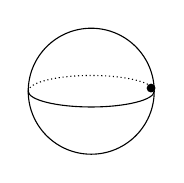
\begin{tikzpicture}[scale=.8]
\draw(0,0)circle(1);
\draw(-1,0)arc[start angle=180,end angle=360,x radius=1,y radius=.25];
\draw[densely dotted](-1,0)arc[start angle=180,end angle=0,x radius=1,y radius=.25];
\fill(.95,.05)circle(2pt);
\end{tikzpicture}}

\sbox{180}{\figure{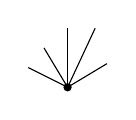
\begin{tikzpicture}[scale=.5]\fill(0,0)circle(3pt);\foreach \x/\y in {-1/.5,-.6/1,0/1.5,.7/1.5,1/.6}{\draw(0,0)--(\x,\y);}\end{tikzpicture}}}
\sbox{181}{\figure{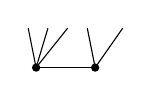
\begin{tikzpicture}[scale=.5]\draw(0,0)--(1.5,0);\fill(0,0)circle(3pt);\fill(1.5,0)circle(3pt);\draw(0,0)--(-.2,1);\draw(0,0)--(.3,1);\draw(0,0)--(.8,1);\draw(1.5,0)--(1.3,1);\draw(1.5,0)--(2.2,1);\end{tikzpicture}}}
\sbox{182}{\figure{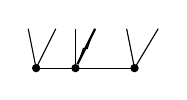
\begin{tikzpicture}[scale=.5]\draw(0,0)--(1,0)--(2.5,0);\foreach \x in {0,1,2.5}{\fill(\x,0)circle(3pt);}\draw(0,0)--(-.2,1);\draw(0,0)--(.5,1);\draw(1,0)--(1,1);\draw[thick](1.05,.1)--(1.5,1);\draw(1.1,.2)--(1.2,.5)--(1.3,.5)--(1.4,.8);\draw(2.5,0)--(2.3,1);\draw(2.5,0)--(3.1,1);\end{tikzpicture}}}
\diagram{\begin{tikzcd}[ampersand replacement=\&,column sep=large,row sep=large]
\text{dim mod}\&2\&1\&0\\
\&
\figure{\usebox{180}}
\&
\figure{\usebox{181}}
\&
\figure{\usebox{182}}\\
\text{nb comp.}\&1\&10\&15\\
\begin{gathered}\text{nb réalisations}\\\text{\unsure{modulaires}}\\\deleted{\text{\unsure{polyédriques}}}\end{gathered}
\&12\&
\begin{gathered}10\times3\times2\\=60\ \unsure{(}\\+10\times2\times6=120\\
\deleted{\text{\unsure{tétraèdre-pyramide}}}\\
(\text{\unsure{tétraèdre}-pointées})\end{gathered}\arrow[uu,bend right=35]
\&15\times2\times2=60
\\
\deleted{\text{\unsure{les types}}}\\
\text{\uline{NB} Nb de structures}\&
\text{pyramidales}:5\times3\times2=30\arrow[uuuurr,bend right=55]\&\\
\&\text{bitétraédrales}:10\times2=20\&
\end{tikzcd}}



\figure{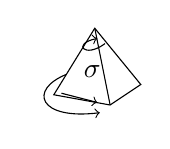
\begin{tikzpicture}[scale=.65]
\draw(0,1.3)--(-.8,0)--(.3,-.2)--(.9,.2)--cycle;
\draw(0,1.3)--(.3,-.2);
\draw[->](-.65,.03)--(.05,-.15);
\draw[->](-.55,.4)..controls(-1.3,.1)and(-1.1,-.5)..(.1,-.35);
\draw[->](.2,1)..controls(-.2,.7)and(-.45,1)..(.05,1.1);
\node at(-.05,.45){$\unsure{\sigma}$};
\end{tikzpicture}}
\mspage{35}
\scanpage{37}
\mspage{36}
le carré est
\[
 \lambda=\frac{(\xi+\eta)^2}{\xi\wedge\eta}
 =\deleted{\unsure{\frac{\xi}{\eta}}}\frac{\xi}{\eta}+\frac{\eta}{\xi}+2
\]
et dont la connaissance nous permet de retrouver la situation de départ à iso.
\deleted{\unsure{près}}\uline{unique} près. La condition à mettre sur
$\lambda$ est que $\lambda-4\ne0$ i.e.
\[
 \unsure{\lambda''|\lambda'}\underset{\unsure{\mathrm{df}}}{=}\lambda-
 \unsure{2}= \frac{\xi}{\eta}+\frac{\eta}{\xi}\ne2.
\]
En termes d'une base \deleted{\unsure{de}} $e_1$ de $L_1$,
satisfaisant $e_1^4=e=\xi\wedge\eta$, donnant une base $e_1^2$ de $L_2$,
la situation est déterminée par \inserted{la paire d'éléments distincts}
$\xi_0,\eta_0\in\mathbb C$ $(\xi=\xi_0e_1^2,\ \eta=\eta_0e_1^2)$,
satisfaisant $\xi_0\eta_0=1$, ou encore par
$\mu=\xi_0+\eta_0\in\mathbb C$ satisfaisant $\mu^2-4\ne0$,
$\xi_0$ et $\eta_0$ se récupérant comme solutions de l'équation
\[
 z^2-\mu z+1=0,
\]
l'équation $\uline{\mu^2-4\ne0\quad\text{i.e.}\quad\unsure{\mu^2|\mu}\ne\pm2}$
s'exprime par les \inserted{2} solutions sont distinctes (néct non nulles car leur
produit est $1$). \deleted{\unsure{Les}} On récupère $I$ comme l'ens des solutions de
\[
 z^4-\mu z^2+1=0
\]
\[
 I=\left\{\pm\sqrt{\tfrac12\left(\mu\pm\sqrt{\mu^2-4}\right)}\right\}
 =\left\{\pm\sqrt{\mu'\pm\sqrt{\mu'^2-1}}\right\}.
\]
\margin{où $\mu'=\tfrac12\mu$ i.e.}
\unsure{\texttt{TRACE}} \illegible{3} \unsure{\texttt{1120}}
\illegible{2} \unsure{\texttt{PLUN3}} \illegible{3}

\unsure{\texttt{JCL}} \illegible{2}
\unsure{\texttt{A105 DE NUMERO}}

\texttt{********************************************************}

\unsure{\texttt{CLEF}} \illegible{8}

\unsure{\texttt{ENJ*0*}} \illegible{7}

\unsure{\texttt{ERAF 1}} \illegible{1}
\unsure{\texttt{1 120 100 301 000 020}}

\unsure{\texttt{AUEF 1 CH0*0*54 6225 A00*FLA9}}
\illegible{2} \unsure{\texttt{16 819}}

\unsure{\texttt{C7L*837}} \illegible{2}
\unsure{\texttt{1 1 26 9 1001111}} \illegible{1}

\unsure{\texttt{ERAF 1}} \illegible{6}

\unsure{\texttt{R8*PH19 CH0*0*37 6250 AGS 00900 6 16}}
\illegible{2} \unsure{\texttt{842}}
\scanpage{38}
\uline{Autom d'ordre deux d'une sphère holomorphe \inserted{$\Sigma$} à
\inserted{un $K$ de} $5$ pts marqués} : Un pt fixe exactement dans $K$,
soit $K=\{P\}\amalg I$, et $\Sigma$ est munie de $I$ et d'un autom
\inserted{$\sigma$} d'ordre $2$, stabilisant $I$,
\inserted{$I$ ne contenant pas de pt fixe de $\sigma$.}
Donc cel. revient à la donnée

a) D'une sphère hol. $\Sigma$, un autom \inserted{$\sigma$} d'ordre $2$
et un pt fixe marqué --- appelant celui-ci $\infty$, et l'autre pt fixe $0$,
cela revient à la donnée d'un torseur $T_1\ (= \Sigma\setminus\{0,\infty\})$
sous $\mathbb C^*$, i.e. d'une droite vectorielle complexe $L_1$
$(T_1=L_1^*)$

b) D'une paire d'orbites \inserted{(distinctes)} de
$\{\pm1\}\subset\mathbb C^*$ opérant sur $T_1=L_1^*$.
Introduisant $T_2=T^{\wedge2}\simeq L_2^*$, où
$L_2=L_1^{\otimes2}$, cel revient à la donnée d'une paire de pts
\inserted{$\{\xi,\eta\}$} (distincts) de $T_2$.
Considérons alors le pt
\[
 e=\xi\wedge\eta=\eta\wedge\xi
 \in T_4=T^{\wedge4}\simeq L_4^*
 \quad(\text{où }L_4=L_1^{\otimes4})
\]
on a donc un
\[
 \mathrm{iso.}\quad T^{\wedge4}\simeq\mathbf1_{\mathbb C^*}
\]
d'où une réduction du groupe structural \inserted{de $T$}
de $\mathbb C^*$ : $\mu_4(\mathbb C^*)\simeq\mathbb Z/4\mathbb Z$.
On peut dire que la donnée de $\{\xi,\eta\}$ revient à celle de
$e=\xi\wedge\eta\inserted{\in T_4}$ et de
$\xi+\eta\in\unsure{L_2}$, soumis à la condition que
$(\xi+\eta)^2-4\xi\eta\ne0$ \deleted{\unsure{un}}.
Notons \deleted{$\unsure{\xi^2+\eta^2-2\xi\eta\ne}$}
que $T_2$ admet une réduction du groupe structural $\mathbb C^*$ :
$\{\pm1\}$, par la \unsure{bibase} $\pm\sqrt e$, donc $\xi+\eta$
définit un \unsure{élt} de $\mathbb C$ à un signe près, dont
\deleted{$(\xi+\eta)^2$}
\mspage{37}
\unsure{\texttt{00 00}} \illegible{4} \unsure{\texttt{CLJ}}
\illegible{3}

\unsure{\texttt{5 12 15 SIGNES LIGNES}}

\unsure{\texttt{FM}} \illegible{2} \unsure{\texttt{LIGNES}}

\unsure{\texttt{CTRL}}

\unsure{\texttt{DEBUT DU TRAITEMENT}}

\unsure{\texttt{FIN DU TRAITEMENT}}

\unsure{\texttt{DUREE}} \illegible{1} \unsure{\texttt{SEC}}

\unsure{\texttt{2}} \illegible{2}

\unsure{\texttt{0}}

\unsure{\texttt{16.18 TOTL}} \illegible{1}
\unsure{\texttt{880 30.53 45.63 PLUM 0}}

\unsure{\texttt{16.852 4}}

\unsure{\texttt{16.52 1}}

\unsure{\texttt{19.11 TOTL949 1840 74.212 40.33 PLUME 0}}

\unsure{\texttt{19.426 4}}
\scanpage{39}
Changer la base $e_1$ en $\zeta e_1$ $(\text{où }\zeta^4=1)$
\deleted{revient à changer \unsure{par}}
$\{\xi,\eta\}$ en $\{\zeta^2\xi,\zeta^2\eta\}$, donc $\mu$ en
$\zeta^2\mu$, qui est donc égal à $\mu$ si $\zeta\in\{\pm1\}$,
égal à $-\mu$ si $\zeta\in\{\pm i\}$.

La multiplicité modulaire pour les structures envisagées,
\uline{rigidifiées} par la donnée de $e_1$, est donc
$\mathbb P^1\setminus\{0,\pm2,\infty\}$.
Elle s'envoie dans la multiplicité $M_{0,5}$ --- il y a lieu de
regarder l'effet sur les groupoïdes fondamentaux.
\unsure{\texttt{000000}}\illegible{3}
\diagram{\(\begin{array}{lll}
\unsure{\texttt{00000000}} & \unsure{\texttt{00000000}} & \unsure{\texttt{00000000}}\\
\unsure{\texttt{0000000000}} & \unsure{\texttt{0000000000}} & \unsure{\texttt{0000000000}}\\
\unsure{\texttt{00\ \ \ \ \ \ \ 00}} & \unsure{\texttt{00\ \ \ \ \ \ \ 00}} & \unsure{\texttt{00\ \ \ \ \ \ \ 00}}\\
\unsure{\texttt{00\ \ \ \ \ \ \ 00}} & \unsure{\texttt{00\ \ \ \ \ \ \ 00}} & \unsure{\texttt{00\ \ \ \ \ \ \ 00}}\\
\unsure{\texttt{00\ \ \ \ \ \ \ 00}} & \unsure{\texttt{00\ \ \ \ \ \ \ 00}} & \unsure{\texttt{00\ \ \ \ \ \ \ 00}}\\
\unsure{\texttt{00000000}} & \unsure{\texttt{00000000}} & \unsure{\texttt{00\ \ \ \ \ \ \ 00}}\\
\unsure{\texttt{00000000}} & \unsure{\texttt{00000000}} & \unsure{\texttt{00\ \ \ \ \ \ \ 00}}\\
\unsure{\texttt{00\ \ \ \ \ \ \ 00}} & \unsure{\texttt{00\ \ \ \ \ \ \ 00}} & \unsure{\texttt{00\ \ \ \ \ \ \ 00}}\\
\unsure{\texttt{00\ \ \ \ \ \ \ 00}} & \unsure{\texttt{00\ \ \ \ \ \ \ 00}} & \unsure{\texttt{00\ \ \ \ \ \ \ 00}}\\
\unsure{\texttt{00\ \ \ \ \ \ \ 00}} & \unsure{\texttt{00\ \ \ \ \ \ \ 00}} & \unsure{\texttt{00\ \ \ \ \ \ \ 00}}\\
\unsure{\texttt{0000000000}} & \unsure{\texttt{0000000000}} & \unsure{\texttt{0000000000}}\\
\unsure{\texttt{00000000}} & \unsure{\texttt{00000000}} & \unsure{\texttt{00000000}}\\
\end{array}\)}
\diagram{\(\begin{array}{llll}
\unsure{\texttt{PPPPPPPPPP}} & \unsure{\texttt{LL}} & \unsure{\texttt{OOOOOOOO}} & \unsure{\texttt{TTTTTTTTTTTT}}\\
\unsure{\texttt{PPPPPPPPPPPP}} & \unsure{\texttt{LL}} & \unsure{\texttt{OOOOOOOOOO}} & \unsure{\texttt{TTTTTTTTTTTT}}\\
\unsure{\texttt{PP\ \ \ \ \ \ \ PP}} & \unsure{\texttt{LL}} & \unsure{\texttt{OO\ \ \ \ \ \ \ OO}} & \unsure{\texttt{TT}}\\
\unsure{\texttt{PP\ \ \ \ \ \ \ PP}} & \unsure{\texttt{LL}} & \unsure{\texttt{OO\ \ \ \ \ \ \ OO}} & \unsure{\texttt{TT}}\\
\unsure{\texttt{PP\ \ \ \ \ \ \ PP}} & \unsure{\texttt{LL}} & \unsure{\texttt{OO\ \ \ \ \ \ \ OO}} & \unsure{\texttt{TT}}\\
\unsure{\texttt{PPPPPPPPPPPP}} & \unsure{\texttt{LL}} & \unsure{\texttt{OO\ \ \ \ \ \ \ OO}} & \unsure{\texttt{TT}}\\
\unsure{\texttt{PPPPPPPPPP}} & \unsure{\texttt{LL}} & \unsure{\texttt{OO\ \ \ \ \ \ \ OO}} & \unsure{\texttt{TT}}\\
\unsure{\texttt{PP}} & \unsure{\texttt{LL}} & \unsure{\texttt{OO\ \ \ \ \ \ \ OO}} & \unsure{\texttt{TT}}\\
\unsure{\texttt{PP}} & \unsure{\texttt{LL}} & \unsure{\texttt{OO\ \ \ \ \ \ \ OO}} & \unsure{\texttt{TT}}\\
\unsure{\texttt{PP}} & \unsure{\texttt{LL}} & \unsure{\texttt{OO\ \ \ \ \ \ \ OO}} & \unsure{\texttt{TT}}\\
\unsure{\texttt{PP}} & \unsure{\texttt{LLLLLLLLLLLL}} & \unsure{\texttt{OOOOOOOOOO}} & \unsure{\texttt{TT}}\\
\unsure{\texttt{PP}} & \unsure{\texttt{LLLLLLLLLLLL}} & \unsure{\texttt{OOOOOOOO}} & \unsure{\texttt{TT}}\\
\end{array}\)}
\texttt{****A START JOB 880 PLOTEDIT }\illegible{5}\texttt{ ROOM}

\texttt{****A START JOB 880 PLOTEDIT }\illegible{5}\texttt{ ROOM}

\texttt{****A START JOB 880 PLOTEDIT }\illegible{5}\texttt{ ROOM}

\texttt{****A START JOB 880 PLOTEDIT }\illegible{5}\texttt{ ROOM}

\texttt{****A START JOB 880 PLOTEDIT }\illegible{5}\texttt{ ROOM}

\texttt{****A START JOB 880 PLOTEDIT }\illegible{5}\texttt{ ROOM}

\texttt{DERNIERE MISE A JOUR DE JOURNAL : 11-06-82}
\mspage{38}
\scanpage{40}
Catalogue des opérations élémentaires dans $\unsure{\mathrm{RCD}_{\mathrm{top}}|\mathrm{RTD}_{\mathrm{top}}}$
\mspage{39}
\scanpage{41}
\texttt{/*JOB=CRAY2,ACCT=*********,ALL=M06}\qquad\texttt{J0231CNU}

\texttt{// JOB MSGLEVEL=(0,0),MSGCLASS=Z}

\texttt{// EXEC CSSBATCH}

\texttt{//CRAYIN DD *}

\uline{Oct. 4 83}

\diagram{\begin{tikzcd}[ampersand replacement=\&,column sep=large,row sep=large]
\unsure{\mathbb R}=\unsure{RR}/\sigma_1\arrow[d]\&
\overset{\sigma_0,\sigma_1}{\unsure{RR}}\arrow[l]\arrow[d,"\mathrm{supp}"]\\
A=\vec A/\sigma\&
\vec A\arrow[l]\arrow[loop below,"\sigma"]\&
\vec A_0\arrow[l,leftrightarrow]\arrow[d,"\sigma"]\\
\&\&S\arrow[r,"g"]\&\mathbb N
\end{tikzcd}}

a) $\sigma^2=\mathrm{id}$, $\sigma$ ss pt fixe

b) supp compatible avec $\mathbb D_\infty\longrightarrow\{\pm1\}$

c) $\unsure{RR}/\mathbb D_\infty\underset{\unsure{\exists!}}{\longleftrightarrow}
 A=\vec A/\{\pm1\}$

d) (\unsure{évt}) condition additionnelle (cs hyperboliques) :
$\forall s\in S$, on a
$\deleted{\unsure{2g(s)}}:\ 2g(s)+\nu_s\ge3$
\margin{\[
3\unsure{g_s|g_p}-3+\nu_s\ge0
\]
\[
2\unsure{g_s|g_p}-2+\nu_s\ge1
\]
\[
2g_s+\nu_s\ge3
\]}

1) Somme $+$

\diagram{\(\begin{array}{rl}
4)\ \big\{&\text{amalgamation (\uline{\unsure{sous|sans}} gommage)}\\
5)&\text{découpage (en gardant données de recollement)}\\[1ex]
2)\ \big\{&\text{gommage de \deleted{\unsure{repères}} sommets de marquage.}\\
3)&\text{surmarquage}
\end{array}\)}
\figure{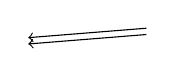
\begin{tikzpicture}
\draw[<-] (0,0)--(1.5,.12);\draw[<-] (0,-.08)--(1.5,.04);
\end{tikzpicture}}
6) Bouchage des trous (gommage des cercles de raccord)

7) \uline{gommage} de cercles de découpage

\margin{4,5 inverses l'un de l'autre (à condition que l'on ne découpe que par
des cercles \uline{marqués})}

\margin{\uline{Cercles de découpage}

\uline{Cercles de raccord}

Sommets de marquage \unsure{ou rigidification|antirigidification}
$\left\{\begin{array}{l}\text{périphériques}\\\text{intérieurs}\end{array}\right.$

Cercles marqués (non marqués)}
\margin{\uline{graphes pondérés}

graphes bipondérés \deleted{\unsure{marqués}}

graphes pondérés marqués}

\uline{Le foncteur twist} $\tau_r$ $(r\in\mathbb Q)$ relatif à un cercle de
découpage marqué, est défini en termes de 4) 5), avec
$\tau_r=\mathrm{id}$ si $r\in\mathbb Z$.
\diagram{\fbox{\begin{tikzcd}[ampersand replacement=\&]
S_1\unsure{\mathcal T}_{g,\nu}^{\pm1}\arrow[r]\&
\unsure{\mathcal T}_{g,\nu}^{\pm1}\arrow[r]\&
\mathrm{Ens}(\unsure{\nu})\times\unsure{[\pm1]|[\mathrm I\mid J]}
\end{tikzcd}}}
\deleted{$\unsure{\mathcal T_{g,\nu}^{\pm}\ \mathcal T_{\mathrm{top}}\
(TSD)_{g,\nu}}$}
\[
\unsure{T_{g,\nu}S_\alpha}
\]

Mais l'\uline{iso} de \uline{twist} \deleted{\unsure{est un}} relatif à
un cercle (de découpage ou de raccord, marqué ou pas),
\inserted{\unsure{ou de recollement}}
$\tau_r$ (pour un cercle de découpage) est une
\uline{nouvelle opération} \unsure{importante}.

\margin{type combinatoire d'un objet de
$\deleted{\unsure{\mathcal T}},\ SD\unsure{\mathcal T}_{\mathrm{top}}$

Catégorie des types combinatoires

\diagram{\(\begin{array}{cc}
\deleted{\mathcal T S}&\deleted{\mathcal T D}\\
\multicolumn{2}{c}{\deleted{\mathcal T SD}}
\end{array}\)}
$\unsure{\text{avec inv}}^{\pm}$
\deleted{$\unsure{\mathcal T^*(\Gamma)}$}

$\unsure{\mathcal T}$

\diagram{\(\begin{array}{c|c}
S\mathcal T&ST\\
SD\mathcal T&SDT\\
D\mathcal T&DT
\end{array}\)}

\diagram{\begin{tikzcd}[ampersand replacement=\&,column sep=small]
\&\mathcal T\arrow[dl,dash]\arrow[dr,dash]\&
\text{graphes pond. discrets}\\
S\mathcal T\arrow[dr,dash]\& \&D\mathcal T\arrow[dl,dash]\\
\&SD\mathcal T\&
\end{tikzcd}}
\unsure{graphes b}\qquad\text{graphes pondérés}\qquad\text{graphes}

\diagram{\begin{tikzcd}[ampersand replacement=\&,column sep=small]
\&t\arrow[dl,dash]\arrow[dr,dash]\&\\
st\arrow[dr,dash]\&\&dt\arrow[dl,dash]\\
\&sdt\&
\end{tikzcd}}}
\mspage{40}
\scanpage{42}
opérations de recollage / sommes

Objets; diagrammes

\diagram{\(\begin{array}{l}
\left\{\begin{array}{l}
\text{cercles de raccord (ou de recollage)}\\
\text{cercles de découpage}
\end{array}\right.\\
\text{Sommets de \uline{marquage} (périphériques, intérieurs)}\\
\text{cercles marqués et non marqués}
\end{array}\)}

[condition \deleted{\unsure{de}} ``\unsure{anabélienne}'' ou de ``stabilité'']

\diagram{\begin{tikzcd}[ampersand replacement=\&,column sep=small,row sep=small]
\&\deleted{\unsure{SD}}\unsure{\mathcal T}\arrow[dl,dash]\arrow[dr,dash]\arrow[rrr]\&\&\&t\arrow[dl,dash]\arrow[dr,dash]\&\\
S\mathcal T\arrow[dr,dash]\arrow[rr,dash]\arrow[rrr,bend left=20]\&\&
D\mathcal T\arrow[dl,dash]\arrow[rrr,bend right=20]\&
st\arrow[dr,dash]\&\&dt\arrow[dl,dash]\\
\&SD\mathcal T\arrow[rrr]\&\&\&sdt\&
\end{tikzcd}}
\margin{types combinatoires}

Catalogue opérations $+$ structures

\diagram{\(\begin{array}{rl}
1)\ \left.\vphantom{\begin{array}{l}1\\2\\3\end{array}}\right\{&
\text{Somme}\\
2)&\text{gommage (partiel) de marquage}\quad\updownarrow\\
3)&\text{surmarquage}\\[1ex]
4)\ \left.\vphantom{\begin{array}{l}4\\5\\6\end{array}}\right\{&
\text{découpage (partiel),}\\
5)&\text{\uline{amalgamation} ou recollage
(\deleted{\unsure{avec données de}}\inserted{sans gommage!})}\quad\updownarrow\\
6)&\text{bouchage de trous (= gommage de cercles de raccord)}\\
7)&\text{gommage de cercles intérieurs}
\end{array}\)}

foncteurs et iso ``twist''
\mspage{41}
\scanpage{43}
les divers avatars principaux de la Tour de Teichmüller :
\deleted{systèmes de groupoïdes}

groupoïde $\mathrm{RTD}_{\ldots}$ avec structures
\inserted{(``les 10 opérations'')}, \unsure{réalis.} diverses dans un groupoïde
dont le \deleted{\unsure{représentant}} le plus élémentaire est
$\deleted{\unsure{\mathrm{RTD}}},\ \unsure{\mathbb T}_{\mathrm{top}}$

\diagram{\begin{tikzcd}[ampersand replacement=\&,row sep=large,column sep=large]
\&\unsure{\mathbb T}_{\mathrm{top}}\&
\begin{gathered}\text{cas topologique (à bord \deleted{\unsure{géod.}} torique)}\\
\text{découpage top.}\end{gathered}\\
\mathbb T'_{\mathrm{diff}}\arrow[r,shift left]\arrow[from=r,shift left]\&
\mathbb T_{\mathrm{diff}}\arrow[u]\&
\begin{gathered}\text{cas différentiable (à \deleted{pts \unsure{trous} pointés}}\\
\text{\inserted{bord. toriques})}\\
\deleted{\text{(avec \unsure{presque} pts marqués)}}\qquad\text{déc. diff}\end{gathered}\\
\&\mathbb T_{\mathrm{an}}\arrow[u]\&
\begin{gathered}\text{cas }\mathbb C\text{-analytique (à bord \unsure{torique})}\\
\text{déc. en }\unsure{\mathbb C^\infty?}\end{gathered}\\
\mathbb T'_{\mathrm{an}}\arrow[uu,"\begin{gathered}\text{à pts marqués}\\
\text{et \unsure{drs.} tangts}\\\text{complexes}\\\text{\unsure{qconq.}}\end{gathered}"]
\arrow[ur,shift left]\arrow[from=ur,shift left]\&\&\\
\mathbb T'_{\mathrm{hyp}}\arrow[u]\arrow[r,shift left]\arrow[from=r,shift left]\&
\mathbb T_{\mathrm{hyp}}\arrow[uu]\&
\begin{gathered}\text{cas hyperbolique (à bord géodésique)}\\
\text{déc. en géod.}\end{gathered}\\
\&\mathbb T_{\mathbb C\mathrm{alg}}\arrow[u]\&
\begin{gathered}
\text{cas }\mathbb C\text{-algébrique (courbes ND,}\\
\text{munies d'une \deleted{rigidification} de}\\
\text{\unsure{propagation du cercle} aux pts}\\
\text{doubles, plus pts marqués}
\end{gathered}\\
\&\mathbb T_{\overline{\mathbb Q}\text{-}\mathrm{alg}}\arrow[u]\&
\begin{gathered}\text{cas }\overline{\mathbb Q}\text{-alg. (\unsure{pour opération|pour y obtenir}}\\
\text{\unsure{dessus via|des sections}}\ \unsure{\mathrm{Gal}/\mathbb Q}\text{)}\end{gathered}\\
\&\mathbb T_{\mathrm{comb}}\arrow[u]\&
\begin{gathered}\text{cas combinatoire, via cartes \unsure{sèches}}\\
\text{\uline{à bord} \unsure{quadr.}, avec sommets marqués}\end{gathered}\\
\&\mathbb T_{\unsure{\mathrm{L\acute ego}}}\arrow[u]\&
\begin{gathered}\text{cas combinatoire ``Légo'', avec}\\
\text{les 10 piliers en jeu}\end{gathered}\\
\&\mathbb T_{\mathrm P}\arrow[u]\&
\begin{gathered}\text{cas combinatoire ``\unsure{pantalonique}'',}\\
\text{avec une seule pièce \unsure{dite}}\\
\text{\deleted{``pantalon''} triade.}\end{gathered}
\end{tikzcd}}
\mspage{42}
\unsure{\texttt{24 CNU}}\illegible{1}

\illegible{7}

\illegible{6}

\illegible{8}

\unsure{\texttt{POUR}}\illegible{5}

\illegible{9}

\unsure{\texttt{ECRIT PAR}}\illegible{3}\unsure{\texttt{INFORMATION}}\illegible{3}

\illegible{8}

\unsure{\texttt{TINT}}\illegible{5}

\unsure{\texttt{UTILISER}}\illegible{4}
\scanpage{44}
\mspage{1}
\uline{Groupoïdes de Teichmüller.}

\textcircled{1} Cas topologique.

La variante la plus simple est
\[
\mathcal T^+_{\mathrm{top}}\quad\text{ou}\quad\mathcal T_{\mathrm{top}}
\]
(\uline{groupoïde de Teichmüller \uuline{orienté} topologique})

\uline{Objets} : surfaces \uline{à bord} compactes orientées $(\Sigma)$.

\uline{flèches} : classes d'isotopie d'iso (conservant l'orientation)

\margin{Finalement, \unsure{tout pris en détail}, \unsure{au} point de vue
\unsure{œcuménique}, il semble que c'est le cas $\mathcal T^\pm$ qui offre
le plus \unsure{utilité}; \deleted{\unsure{d'où}} c'est lui qui
\unsure{aura} donc ici la notation la plus simple $\mathcal T$,
et le \unsure{groupe} orienté s'appelle $\mathcal T^+$.}

Variante immédiate
\[
\mathcal T_{\mathrm{top}}^\pm
\]
(\uline{groupoïde de Teichmüller \uuline{biorienté} topologique}) :
mêmes objets, flèches sont les classes d'isotopie d'homéomorphismes
(ne conservant pas néct. l'orientation).

Soit $[\pm1]$ le groupoïde ayant un seul objet $e$ (par exemple $e=\varnothing$)
et comme groupe d'autom $\pm1$. On a un morphisme de signature
\diagram{\begin{tikzcd}[ampersand replacement=\&]
\mathcal T^\pm_{\mathrm{top}}\arrow[r,"\chi"]\&{[\pm1]}
\end{tikzcd}}
dont la \uline{fibre} \deleted{est} (ou noyau) est
$\mathcal T_{\mathrm{top}}^+=\mathcal T_{\mathrm{top}}$.
\margin{\unsure{Ceci n'a un sens} \unsure{qu'}à des surfaces connexes!}

La variante la plus complexe est
\[
S_*\mathcal TD_{\mathrm{top}}^+\quad\text{ou}\quad
S_*\mathcal TD_{\mathrm{top}},
\]
``\uline{groupoïde de Teichmüller \inserted{orienté} spécial dévissé topologique}''
\mspage{43}
\scanpage{45}
\deleted{On a ainsi la notion de \uline{graphe pondéré}
\uline{enrichi} (pondéré par $\unsure{g|\gamma}$, la structure}
\mspage{44}
\scanpage{46}
\mspage{2}
\uline{Objets} : Triples $(X,\widetilde\Sigma,
\deleted{\unsure{S}}\inserted{R})$, où

$X$ surface à bord compacte orientée

$\widetilde\Sigma$ sous-variété compacte de $X$
\deleted{\unsure{close}}, $\widetilde\Sigma\supset\partial X$

$\deleted{\unsure{S}}R\subset\Sigma\deleted{\unsure{\widetilde\Sigma}}$,
partie finie

\margin{$X,\unsure{\partial X},\Sigma,S$}
\margin{$\widetilde\Sigma=\partial X\amalg\Sigma$

On peut considérer que $R$ rigidifie $\widetilde\Sigma$ :
que $R$ ``découpe'' $\widetilde\Sigma$.}

\uline{flèches} : classes d'isotopie d'homéom. conservant l'orientation

\deleted{Variante \unsure{de}}
Les composantes connexes de $\widetilde\Sigma\setminus\partial X
\inserted{=\Sigma}$ sont les \uline{cercles de découpage},
\inserted{celles de $\partial X$ sont les cercles de raccord},
les éléments de $\deleted{\unsure{S}}R$ sont les
\deleted{\unsure{pts de marquage}} \uline{sommets de
\deleted{marquage}\inserted{rigidification}},
\deleted{(ou de rigidification)},
\deleted{les composantes connexes de $\partial X$ sont les ``trous''.}
Les composantes connexes de $X$ sont les
$\deleted{\text{connexes}}$\inserted{\uline{composants}}
de l'objet envisagé.

Variante $S_*\mathcal TD_{\mathrm{top}}^\pm$, avec
\diagram{\begin{tikzcd}[ampersand replacement=\&]
S_*\mathcal TD_{\mathrm{top}}\arrow[r,phantom,"\subset"]\&
S_*\mathcal TD_{\mathrm{top}}^\pm\arrow[r]\&{[\pm1]}
\end{tikzcd}}
comme tantôt.

On a des sous-groupoïdes pleins
\diagram{\(\begin{array}{ccl}
R=\varnothing,\ \Sigma=\unsure{\varnothing}&
\mathcal T_{\mathrm{top}}\quad\text{et}\quad\mathcal T^\pm_{\mathrm{top}}&\\
\deleted{\unsure{R=\widetilde\Sigma=\varnothing}}&&\\
\Sigma=\deleted{\unsure{\partial X}}\varnothing&
S_*\mathcal T_{\mathrm{top}}\quad\text{et}\quad S_*\mathcal T^\pm_{\mathrm{top}}&
\begin{gathered}
\text{(groupoïdes de Teichmüller \uline{spéciaux}}\\
\text{\inserted{ou \uline{rigidifiés}} (topologiques orientés))}
\end{gathered}\\
R\text{ quelconque}&&\\
R=\varnothing&
\mathcal TD_{\mathrm{top}}\quad\text{et}\quad\mathcal T^\pm D_{\mathrm{top}}&
\end{array}\)}
(Cas pas intéressant je crois, sauf pour $\Sigma=\unsure{\varnothing}$
également)

\margin{MD = ``modulaire'' ! Mumford--Deligne}

\deleted{\unsure{Dé}} \uline{Détermination} du
$\pi_0(S_*\mathcal TD_{\mathrm{top}})
 \xrightarrow{\sim}\pi_0((S_*\mathcal TD)^\pm_{\mathrm{top}})$.

On introduit les \uline{graphes} \deleted{\unsure{MD}} bipondérés
\mspage{45}
\scanpage{47}
\mspage{3)}
qui forment un groupoïde $\deleted{\mathrm{MD}}.\ \mathrm{Grbip}$
ou $(\unsure{\mathrm{Grabipond}})$

Objets : graphes \inserted{finis} $(S,\vec A,\sigma,o)$
\inserted{$+$ structures suppl.},
(pouvant avoir des sommets isolés, des boucles fermées, a fortiori
plusieurs arêtes entre deux sommets, et aussi des ``\uline{arêtes libres}''
\inserted{(``\unsure{non attachées}'' aux \unsure{2})}
correspondant aux pts fixes de $\sigma$)
$S,\vec A$ ens. finis, $\sigma:\vec A\longrightarrow\vec A$ involution,
$o:\vec A\longrightarrow S$ appel. ``origine''.
On se donne de plus
\diagram{\begin{tikzcd}[ampersand replacement=\&]
S\arrow[r,"\deleted{\unsure{g}}\inserted{\unsure{\gamma}}"]\&
\mathbb N
\end{tikzcd}}
(application ``genre'' ou ``poids'')

\diagram{\begin{tikzcd}[ampersand replacement=\&]
\deleted{\unsure{\widetilde A}}=\unsure{A_\ell}
\arrow[r,"\unsure{r\rho_2|\rho}"]\&\mathbb N
\end{tikzcd}}
(application \deleted{\unsure{rigidification}}
``indice de rigidification'')

\deleted{$\unsure{A_\ell}\quad\text{``\unsure{arêtes libres}''}$}
$\underset{\mathrm{def}}{\unsure{A_\ell}\subset\vec A/\sigma}$
\deleted{``\unsure{ensemble des sommets supplémentaires}''}

\margin{pas assez précis comme donnée. La pondération d'une arête doit être
remplacée par celle d'un pol. comb.
$\unsure{T_a}$ avec $\omega(\unsure{T_a})\simeq\omega(a)$.}
\margin{J'ai indiqué une pondération des sommets, mais pas des arêtes}

\figure{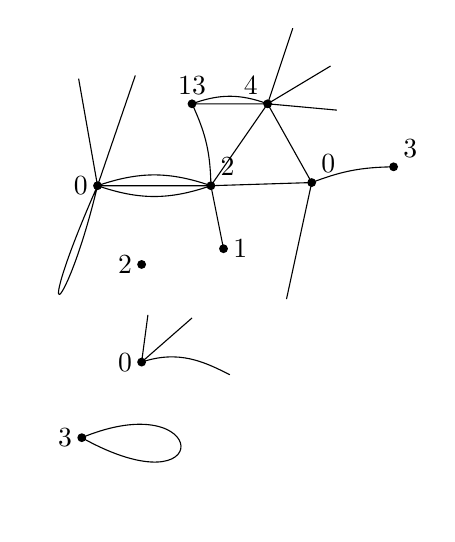
\begin{tikzpicture}[scale=.8]
\coordinate (a) at (0,0); \coordinate (b) at (1.8,0);
\coordinate (c) at (3.4,.05); \coordinate (d) at (2.7,1.3);
\coordinate (e) at (1.5,1.3); \coordinate (f) at (2,-1);
\coordinate (g) at (4.7,.3);
\draw (a)--(b)--(c)--(d)--(b)--(f);
\draw (a) to[bend left=19] (b) (a) to[bend right=19] (b);
\draw (a) .. controls (-1.1,-2.5) and (-.5,-2.1) .. (a);
\draw (a)--(-.3,1.7) (a)--(.6,1.75);
\draw (b) to[bend right=12] (e);
\draw (e)--(d) (e) to[bend left=20] (d);
\draw (d)--(3.1,2.5) (d)--(3.7,1.9) (d)--(3.8,1.2);
\draw (c)--(3,-1.8) (c) to[bend left=10] (g);
\foreach \p/\lab/\pos in {a/0/left,b/2/above right,c/0/above right,d/4/above left,e/13/above,f/1/right,g/3/above right}
{\fill (\p) circle(2pt); \node[\pos] at (\p) {$\lab$};}
\fill (.7,-1.25) circle(2pt); \node[left] at (.7,-1.25) {$2$};
\fill (.7,-2.8) circle(2pt); \node[left] at (.7,-2.8) {$0$};
\draw (.7,-2.8)--(.8,-2.05) (.7,-2.8)--(1.5,-2.1)
(.7,-2.8)..controls(1.3,-2.6)and(1.7,-2.8)..(2.1,-3);
\fill (-.25,-4) circle(2pt); \node[left] at (-.25,-4) {$3$};
\draw (-.25,-4).. controls(1.8,-3.15)and(1.9,-5.2)..(-.25,-4);
\end{tikzpicture}}

\deleted{Ou encore, posons $\widetilde S=S\amalg A_\ell$, identif.
à l'ens de tous les ``sommets'', \deleted{\unsure{marqués}} et
``\uline{marqués}'' (i.e. $\in S$) et les \unsure{trous}
\inserted{(i.e. correspondant à $\alpha\in A_\ell$)}
du graphe, l'on donne
\diagram{\begin{tikzcd}[ampersand replacement=\&]
\widetilde S\arrow[r,"\pi"]\&\mathbb N
\end{tikzcd}}
(\uline{pondération} du graphe)}

\margin{\[
\widetilde S=S\amalg\deleted{\unsure{S_\ell}}\inserted{A_\ell}
\qquad\deleted{\unsure{\mathrm{apparents}}}
\]
\[
\widetilde A=\vec A/\sigma=A\amalg A_\ell.
\]
\diagram{\begin{tikzcd}[ampersand replacement=\&,column sep=small]
\vec A\arrow[d] = \&\underbrace{\vec A_0}_{\vec A\setminus\vec A^\sigma}
\arrow[d,"\deg2"]\amalg\&
\underbrace{\vec A_\ell}_{\vec A^\sigma}\arrow[d,"\deg1"]\\
\widetilde A = \&A\amalg\&A_\ell
\end{tikzcd}}
Ordre d'un sommet
\[
\sigma(s)=\underbrace{\sigma_\ell(s)}_{\substack{\text{correspond aux ``trous''}\\
\text{ou cercles de recollage}}}+\sigma_0(s)
\]}

La donnée du \uline{graphe} sous-jacent à un graphe
$\deleted{\mathrm{MD}}\inserted{\mathrm{bip.}}$ revient à celle d'un graphe
``ordinaire'' correspondant (sans arêtes libres i.e. où $\sigma$ opère
ss pts fixes), i.e.
\[
\left(S,(\vec A\setminus\vec A^\sigma),
 \sigma|(\vec A\setminus\vec A^\sigma),
 o|(\vec A\setminus\vec A^\sigma)\right),
\]
\uline{plus} un ensemble \inserted{fini} $A_\ell$
(\uline{arêtes} libres)
\deleted{ou ``sommets-trous'')} et une application
\diagram{\begin{tikzcd}[ampersand replacement=\&]A_\ell\arrow[r]\&S\end{tikzcd}}

\uline{Flèches} Les iso. de telles structures
\mspage{46}
\scanpage{48}
\mspage{4)}
On a un foncteur
\diagram{\begin{tikzcd}[ampersand replacement=\&]
(*)\quad\Gamma:\quad S_*\mathcal TD^\pm_{\mathrm{top}}\arrow[r]\&
\deleted{\unsure{\mathrm{MD}}}(\mathrm{Grabipond})
\end{tikzcd}}
qui associe à un objet \inserted{$(X,\widetilde\Sigma,R)$} de
$S_*\mathcal TD^\pm_{\mathrm{top}}$ le graphe \inserted{MD}
$(S,\vec A,\sigma,\deleted{\unsure{g}}\inserted{o},\gamma,\rho)$ suivant :
\[
S=\pi_0(X\setminus\widetilde\Sigma)\simeq\pi_0(\text{Déc}(X,\widetilde\Sigma))
\]
$\vec A=$ ens des couples $(C,\deleted{\unsure{\xi}}\omega)$, où
$C\deleted{\in A}\inserted{\in\pi_0(\widetilde\Sigma)}$, et où
$\omega\in\mathrm{Or}(C)\inserted{\simeq\mathrm{rive}_X(C)}$,
soumis à la condition que si $C\in\pi_0(\partial X)$, alors $\omega$
est l'orientation induite i.e. la rive qui se trouve dans $X$.

$\sigma=$ échange des rives (\unsure{quand on a} le droit d'échange,
sinon, i.e. si $C\in\pi_0(\partial X)$, on pose $\sigma(a)=a$)

$\deleted{\unsure{O}}\inserted{o}$ : associe à $(C,\text{rive de }C)$
l'unique ``face'' $\in\pi_0(X\setminus\widetilde\Sigma)$ qui
contient cette rive \deleted{$\unsure{R\subset\widetilde R}$}
\diagram{\begin{tikzcd}[ampersand replacement=\&]
\gamma:\quad S\arrow[r]\arrow[d,equal]\&\mathbb N\\
\pi_0(X\setminus\widetilde\Sigma)\&
\end{tikzcd}}
application \uline{genre} des composants $X_i$.
\diagram{\begin{tikzcd}[ampersand replacement=\&]
\unsure{r|\rho}:\quad A=\pi_0(\widetilde\Sigma)\arrow[r]\&\mathbb N\&
C\arrow[r,mapsto]\&\mathrm{Card}(R\cap C).
\end{tikzcd}}

Le foncteur $(*)$ \deleted{est \unsure{ess.} surjectif et}
\inserted{induit un \uline{iso} sur les} $\pi_0$ et une surjectif
sur les $\pi_1$ (c'est un \uline{0-isomorphisme} \unsure{?},
en langage homotopique).

\deleted{\unsure{La preuve}} :

\uline{Remarque}. Dans $S_*\mathcal TD^\pm_{\mathrm{top}}$ il y a une
opération évidente de \uline{sommes} \inserted{\uline{disjointes}},
dans $\deleted{\mathrm{FMD}}\inserted{\mathrm{Grabipond}}$ aussi,
et $(*)$ y commute.
\mspage{47}
\scanpage{49}
\mspage{5)}
Cette opération de sommes est la plus triviale parmi les opérations qu'il
nous faudra expliciter et transcrire (combinatoirement) dans la suite.
Notons de suite, pour $(X,\widetilde\Sigma,R)$ donné
\[
X\deleted{\unsure{\Sigma}}\text{ connexe}\Longleftrightarrow
\Gamma\mathrm{MD}(X,\widetilde\Sigma,R)\text{ connexe}
\]
plus précisément
\[
\pi_0(X)\simeq\pi_0(\Gamma\mathrm{MD}(X,\widetilde\Sigma,R))
\]
\margin{donner la formule pour le genre d'un
$\alpha\in\pi_0(X)\simeq\pi_0(\Gamma)$ en termes de la pondération ---
plus généralement \unsure{donner} le \uline{genre total} est
\[
g=\sum_{s\in S}g_s+c(\Gamma)
\]
\unsure{indice de connexion} du graphe
$=\deleted{\unsure{\chi}}\unsure{\mathrm{rg}\,H^1(\Gamma)}$.}

\uline{Cas particuliers.}

a) Cas de $S_*\mathcal T^\pm_{\mathrm{top}}\
\deleted{\unsure{S_*\mathcal T_{\mathrm{top}}}}$
--- i.e. $\Sigma=\varnothing$, $\widetilde\Sigma=\partial X$.

Cela correspond au cas des graphes MD \deleted{que} où
\inserted{toutes les arêtes sont libres, i.e.}
tous les sommets sont isolés (sauf arêtes libres)
\deleted{Il} \inserted{Le graphe} est donc déterminé par
\diagram{\begin{tikzcd}[ampersand replacement=\&,column sep=large]
A\ (\simeq\vec A=\vec A^\sigma)\arrow[r,"\unsure{r|\rho}"]\arrow[d]\&\mathbb N\\
S\arrow[r,"\gamma"]\&\mathbb N
\end{tikzcd}}

Le cas de $\mathcal T^\pm_{\mathrm{top}}$ correspond à faire $\rho=0$,
donc la situation est donnée par
\diagram{\begin{tikzcd}[ampersand replacement=\&]
A=\unsure{A_0|A_\ell}\arrow[d]\&\\
S\arrow[r,"\gamma"]\&\mathbb N.
\end{tikzcd}}

\margin{\figure{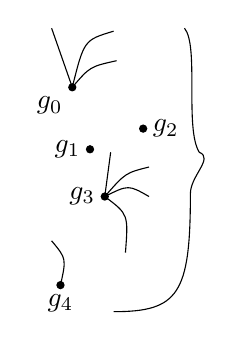
\begin{tikzpicture}[scale=.75]
\fill(0,0)circle(2pt);\node[below left]at(0,0){$g_0$};
\draw(0,0)--(-.35,1) (0,0)..controls(.2,.8)..(.7,.95)
(0,0)..controls(.3,.35)..(.75,.45);
\fill(.3,-1.05)circle(2pt);\node[left]at(.3,-1.05){$g_1$};
\fill(1.2,-.7)circle(2pt);\node[right]at(1.2,-.7){$g_2$};
\fill(.55,-1.85)circle(2pt);\node[left]at(.55,-1.85){$g_3$};
\draw(.55,-1.85)--(.65,-1.1)
(.55,-1.85)..controls(.9,-1.45)..(1.3,-1.35)
(.55,-1.85)..controls(.95,-1.65)..(1.3,-1.85)
(.55,-1.85)..controls(.95,-2.15)..(.9,-2.8);
\fill(-.2,-3.35)circle(2pt);\node[below]at(-.2,-3.35){$g_4$};
\draw(-.2,-3.35)..controls(-.1,-2.9)..(-.35,-2.6);
\draw(1.9,1)..controls(2.15,.7)and(1.9,-.7)..(2.15,-1.1)
..controls(2.4,-1.2)and(2,-1.5)..(2,-1.8)
..controls(2,-3.5)and(1.8,-3.8)..(.7,-3.8);
\end{tikzpicture}}}

Le cas d'une \uline{structure} connexe
$(\mathrm{card.}\,S=1\inserted{\text{ i.e. }S=\{s\}})$
\deleted{type $(g,\nu)$ d'une}
est \deleted{\unsure{homéomorphisme}}\inserted{caractérisé}
par la donnée des deux entiers $(g,\nu)$
$(g=\text{genre},\ \nu=\text{nb de trous})$
\[
g=\gamma(s),\qquad \nu=\mathrm{Card}\,A.
\]
\mspage{48}

\scanpage{50}
\mspage{6}
\uline{Remarque} En fait, on a un foncteur plus précis, vers une catégorie de graphes munis d'une structure où la partie $\rho$ de la pondération est \deleted{\unsure{complétée}} \inserted{remplacée} par une structure plus précise, à savoir \deleted{une \unsure{application}} \deleted{\inserted{une \unsure{famille}}} famille
\[
 \deleted{\unsure{\alpha}\,(\widetilde R,\alpha,p:R\longrightarrow\vec A)}
 \qquad (R_a)_{a\in A}
\]
\deleted{\diagram{\begin{tikzcd}[ampersand replacement=\&,row sep=small]\vec A\arrow[d,two heads]\\ \vec A/\sigma\end{tikzcd}}}
d'ensembles, et pour $\forall a\in A$, si nous désignons l'\unsure{ens} des
\deleted{\unsure{donné d'une permutation de}}
``orientations'' de $a$ ($\operatorname{card}\omega(a)\in\{1,2\}$), une application
\deleted{$R$, et $p$ une application $R\longrightarrow A$ \unsure{conj. à}}
\[
 \omega\longmapsto u_\omega:\quad \omega(a)\longrightarrow\operatorname{Circ}(R_a)
\]
ens des permutations circulaires sur $R_a$
\deleted{et \unsure{d'autre} \unsure{une} \unsure{application injective}}
\[
 \deleted{\unsure{R/\alpha}\lhook\joinrel\longrightarrow\vec A}
\]
avec la condition que si $\omega,\omega'\in\omega(a)$, $\omega\ne\omega'$, alors
\[
 \deleted{u_\omega u_{\omega'}=\operatorname{id}_R}
 \qquad u_{\omega'}=u_\omega^{-1}.
\]
\margin{$\omega(a)\mathrel{\mathop=^{\rm def}}\{\vec a\in\vec A\mid\text{au dessus de }a\}$.}

On peut aussi considérer que la donnée des \unsure{suppléments} revient à la donnée de
\[
 \begin{array}{rcl}
 r:A&\longrightarrow&\mathbb N\\
 a&\longmapsto&\operatorname{Card}p^{-1}(a)
 \end{array}
\]
(la ``pondération-arêtes''), et de donnée d'une famille de torseurs
\[
 (R_a)_{a\in A},\quad \deleted{\unsure{\omega(a)}}
\]
$R_a$ un torseur sous $\mathbb Z/r(a)\mathbb Z\mathbin{\wedge}_{\{\pm1\}}\omega(a)$.
On associe à $(X,\widetilde\Sigma,R)$ une telle structure supplémentaire en prenant
\[
 R_a=R\cap\widetilde\Sigma_a
\]
($\widetilde\Sigma_a$ la comp. connexe de $\widetilde\Sigma$ \deleted{\unsure{marquée}} \inserted{qui correspond à} $a\in A\simeq\pi_0(\widetilde\Sigma)$),
\deleted{$\unsure{R=R(\Sigma C)|R=\pi_0(\widetilde\Sigma)}$, \unsure{$R\longrightarrow S$} \unsure{la donnée de} $\widetilde\Sigma$}
\deleted{\diagram{\begin{tikzcd}[ampersand replacement=\&,row sep=small,column sep=large]
R\arrow[r]\arrow[d,equal]\&S\arrow[d,equal]\\
\unsure{\Gamma}\arrow[r]\&\pi_0(\widetilde\Sigma)
\end{tikzcd}}}
$\omega\longmapsto u_\omega$ défini de façon évidente.
\deleted{et $p$ \unsure{déduit de} \unsure{$(\widetilde\Sigma_a)$} \unsure{sur} $R_a$.}

\uline{NB} Même si $r(\unsure{\omega|a})=1$ ou $r(\unsure{\omega|a})=2$, le fait de disposer
\mspage{49}

\scanpage{51}
\mspage{\deleted{\unsure{6}}7}
d'une structure déjà orientée si $a$ est une arête libre (correspondant à un $C\in\pi_0(\partial X)$), ou qu'on dispose de l'une des deux orientations $\omega(a)$ --- dans le cas où $a$ est une arête ordinaire, implique que l'on tient en mains, pour chaque $a\in A$, un polygone combinatoire $P_a$, dont l'ens des sommets est $R_a$, et l'ens des arêtes peut se décrire \deleted{\unsure{aussi}} de façon canonique en termes de $R_a,\omega_a$ et $\omega_a\longrightarrow\operatorname{Circ}(R_a)$.
Il peut être plus commode dans la donnée d'ensemble de la structure, \unsure{où} la famille des $R_a$ serait unifiée par un
\deleted{qui serait \unsure{les uns un contour}}
\uline{contour combinatoire}, i.e. un ensemble de repères $\vec{\underline R}$ (plutôt ``repères de rigidification''), avec une opération de
\[
 \mathbb D_\infty=\{\sigma_0,\sigma_1\mid\sigma_0^2=\sigma_1^2=1\}
\]
dessus, et une application
\[
 \vec{\underline R}\longrightarrow\vec A
\]
compatible avec l'hom.
\[
 \mathbb D_\infty\xrightarrow{\varepsilon}\{\pm1\}
\]
sur les groupes d'opérateurs, mais de plus un sous ens
\[
 \vec{\underline R}_l^+\subset\vec{\underline R}\mid\vec A_l
\]
définissant une orientation du contour correspondant.
\margin{$(\vec A_l=\text{arêtes libres, correspondant aux cercles de recollements, i.e. les }C\in\pi_0(\unsure{\partial}X))$}
\mspage{50}

\scanpage{52}
\mspage{8}
On a ainsi la notion de \uline{graphe pondéré} \deleted{\unsure{enrichi}} \inserted{\uline{à repères}} $\Gamma$.

\diagram{\begin{tikzcd}[ampersand replacement=\&,column sep=large,row sep=large]
\vec R_l^+\ \deleted{\unsure{\mathbb D_\infty|D_\infty}}\subset\underset{\sigma_0,\sigma_1}{\vec R}
 \arrow[r]\&\vec A\arrow[d,"o"']\arrow[loop right,"\sigma"]\\
\&S\arrow[r,"\gamma"]\&\mathbb N
\end{tikzcd}}

Groupoïde $(\uline{\mathrm{Gr.pondrep}})$

foncteur
\[
 S_*\mathcal TD_{\mathrm{top}}^\pm\longrightarrow(\mathrm{Grpondrep})
\]
qui sera important sans doute dans l'explicitation de l'opération de ``recollement''.
Il est clair en tous cas que toute description algébrico-combinatoire de
$\unsure{S\mathcal TD_{\mathrm{top}}^\pm}$ devra permettre, pour chaque objet de
\deleted{la catégorie} \inserted{groupoïde-}paradigme, de réconstituer (à isom. uniques près) les \uline{graphes pondérés à repères} correspondants.
\inserted{--- plus précisément, il faut réconstituer le foncteur canonique
$S_*\mathcal TD_{\mathrm{top}}^\pm\longrightarrow(\mathrm{Gr.pond.rep.})$
(et non seulement le foncteur à valeurs dans $(\mathrm{Grbipond})$)}

\uline{Opérations essentielles}

A) Opérations ``d'oubli'' ou de ``\uline{gommage}''.

\textcircled{1} \uline{Gommage des repères} À un objet $(X,\Sigma,R)$, muni en plus d'une partie $R'\subset R$, il associe $(X,\Sigma,R\setminus R')$ (gommage de $R'$).
\mspage{51}

\scanpage{53}
\mspage{9}
\uline{NB} Ayant (via un groupoïde équivalent à description purement combinatoire) ``réconstruit''
\deleted{\unsure{du}} \deleted{\unsure{purement}} réalisé le groupoïde
$S\mathcal TD_{\mathrm{top}}^\pm$, et le foncteur
\[
 S\mathcal TD_{\mathrm{top}}^\pm\longrightarrow(\mathrm{Gr.\ pond.\ rep.})
\]
alors on aura par \unsure{cela} aussi \deleted{\unsure{une description}} \inserted{l'équivalent de}
\deleted{de} la donnée d'un $(X,\Sigma,R)$, muni \uline{en plus} d'une partie $R'\subset R$ --- \deleted{\unsure{d'où}} i.e. \unsure{avec} la construction d'un groupoïde \unsure{au-dessus}
\diagram{\begin{tikzcd}[ampersand replacement=\&,row sep=large]
S_*\mathcal TD_{\mathrm{top}}^\pm\
 \left(\begin{gathered}\text{à sous ens. marqué }R'\\
 \text{de sommets-}\\\text{repères}\end{gathered}\right)\arrow[d]\\
S_*\mathcal TD_{\mathrm{top}}^\pm
\end{tikzcd}}
et \deleted{\unsure{d'où}} il nous faudra donc \inserted{décrire} un foncteur ``gommage de $R'$''
\diagram{\begin{tikzcd}[ampersand replacement=\&,column sep=huge]
S_*\mathcal TD_{\mathrm{top}}^\pm
 \left(\underset{\text{marqué}}{\overset{\text{ens}}{R'}}\right)
 \arrow[r,"\text{gommage de }R'"]
 \&S_*\mathcal TD_{\mathrm{top}}^\pm
\end{tikzcd}}
\deleted{Cela s'exprime, sur le}
donnant lieu à un diagramme comm. de foncteurs
\diagram{\begin{tikzcd}[ampersand replacement=\&,row sep=large,column sep=huge]
S_*\mathcal TD_{\mathrm{top}}^\pm(\ldots R'\ldots)
 \arrow[r,"\text{gommage de }R'"]
 \arrow[d,"\text{oubli du }\deleted{\unsure{R'}}\text{ marquage }R'"']
\&S_*\mathcal TD_{\mathrm{top}}^\pm\arrow[dd]\\
S_*\mathcal TD\deleted{\unsure{\#}}_{\mathrm{top}}^\pm\arrow[dr]\\
\&(\mathrm{Gr}\deleted{\mathrm{bi}}\mathrm{pond})
 \arrow[r]\&
 \begin{gathered}\text{graphes avec}\\\text{pondération}\\
 \text{par }\gamma,\text{ mais}\\\text{non par }r,\end{gathered}
\end{tikzcd}}
alors qu'au niveau

\margin{\uline{NB} Cette opération a l'air d'un \uline{affaiblissement} de structure --- mais cet affaiblissement, \unsure{sauf si|si} pour une composante $C$ \unsure{donnée} de $\Sigma^+$, l'on \unsure{doive|doit} ``gommer'' \uline{tous} les repères de \deleted{\unsure{ce}} $C$ --- \unsure{alors} c'est au contraire d'un \unsure{renforcement} de la structure \unsure{qu'il s'agit}, \deleted{\unsure{plutôt}} \unsure{dans le} \unsure{renforcement} \unsure{des nouvelles données|des groupes dans ce cas} --- ou plutôt, des \unsure{groupoïdes} \unsure{du même type} $R'_C=R'\cap C$ \unsure{distincts}, et \unsure{telles} \unsure{catégories isotopiques} \unsure{de type} \unsure{(plus bas)} \unsure{avec d'éventuels} \deleted{\unsure{au dessus de}} \inserted{l'opération} de surmarquage et \unsure{l'autre} sont inverses \unsure{l'un de l'autre}, sont des équivalences de groupoïdes.
Il faudrait \unsure{distinguer les deux cas}, pour distinguer ces \uline{opérations de gommage} \unsure{essentielles|anodines} (qui \unsure{changent le groupe des} \unsure{autom.}) et les \unsure{autres}.}
\mspage{52}

\scanpage{54}
\mspage{10}
des graphes pondérés à repères, l'opération \deleted{\unsure{s'explicite}}
se reflète par une opération correspondante au niveau de $\vec R$, par le ``gommage'' d'une partie $\vec R'$ stable par $\mathbb D_\infty$ i.e. par $\sigma_0,\sigma_1$.

2) Gommage de cercles de découpage.

On se donne maintenant une \deleted{ens. de composantes connexes de} 1-sous-variété
\inserted{(ouv. et)} \inserted{fermée} $\Sigma'$ de $\Sigma\setminus\partial X$,
correspondant à un ensemble \deleted{\unsure{A}} de \deleted{\unsure{comp.}} conn. de $\Sigma'$ i.e. une partie \inserted{$A'_0$} de $\pi_0(\unsure{\Sigma'|\Sigma})=A_0$
(arêtes ordinaires du graphe) --- et on remplace $\Sigma$ par $\Sigma\setminus\Sigma'$.
Au niveau des graphes pondérés, cela se traduit par une opération de \uline{contraction en un point} des arêtes correspondantes, d'où formation d'un nouveau graphe, et d'un \uline{morphisme de générisation} (à l'opposé de ``spécialisation'') de l'ancien vers le nouveau.
Il convient ici d'expliciter comment la pondération suit\ldots\
Au niveau des \deleted{repères} \inserted{sommets}, il est entendu que les sommets repères se trouvant sur $\Sigma'$ sont gommés en $=$ temps --- donc, sur le graphe pondéré à repères, on fait sauter l'ens des repères qui sont au dessus des arêtes $\in\unsure{A'_{0a}|A'_0}$.
\mspage{53}

\scanpage{55}
\mspage{11}
3) \deleted{Gommage} \inserted{Bouchage de trous, ou ``gommage''} de cercles de recollement.

Cette opération est relative à la donnée d'une 1-sous-variété fermée de $\partial X$, i.e. d'une partie $A'_l$ de $\pi_0(\partial X)\simeq A_l$ (ens des arêtes libres du graphe).
Elle consiste à boucher les trous correspondants, au moyen des cônes sur les composantes connexes du bord de $\Sigma'_l$.
Au niveau du graphe, cela consiste à gommer les arêtes libres correspondantes, avec bien entendu aussi les repères de marquage qui se trouvent au dessus --- \deleted{mais} les pondérations des sommets restent inchangées.

\deleted{\unsure{4}}
\uline{Gommage simultané mixte}, \deleted{\unsure{ou}} correspondant à une partie
\deleted{$A\amalg R'$} \inserted{$R'\amalg\Sigma'$} \deleted{quelconque} de $R\amalg\Sigma$,
qui est à la fois ouverte et fermée \inserted{et telle}
\deleted{\unsure{de} $A\amalg\vec R$},
\inserted{que $R'\supset R\cap\Sigma'$},
\deleted{ens. de composantes connexes de $R\amalg\Sigma$},
ou ce qui revient au $=$, une partie \inserted{$R'\amalg A'$} de $R\amalg A$, telle que $R'\supset R\mid A'$.

Au niveau des graphes pondérés à repères, cette opération consiste à exclure \deleted{les} \inserted{de $\vec R$} la partie corr. $\vec R'$, à contracter en un point les arêtes de $A'_{\deleted{\unsure{pq}}}$ (aussi bien libres que \unsure{liées}), en faisant suivre la pondération.
\mspage{54}

\scanpage{56}
\mspage{12}
\deleted{\unsure{A)}} \inserted{(B)}
\uline{Opération} de \deleted{\uline{\unsure{raffinement} de}} \inserted{sur}\uline{marquage}

\deleted{On peut le définir \inserted{en termes de} par la donnée, d'une \unsure{composante connexe de} pour chaque arête du contour $R$, \unsure{$R\ne\varnothing$} $\Sigma\setminus R$. Soit \unsure{$\widetilde\Sigma_*$} $A_0^+\in\unsure{A_0}$ l'ens}
\deleted{\unsure{des}}
Soit $A^+$ l'ens des arêtes \inserted{(libres ou liées)} ``effectivement marquées'', \inserted{i.e. telles que $r(a)>0$},
\deleted{et $B$ l'ens des},
correspondant à des $C\in\pi_0(\Sigma)$ telles que $C\cap R\ne\varnothing$, soit $B^+$ l'ens des comp. connexes de
\[
 \Sigma^+\setminus R\cap\Sigma^+
\]
(lesquelles sont des int. ouverts), un surmarquage est défini par la donnée d'une application
\[
 B^+\xrightarrow{r'}\mathbb N,
\]
et peut se décrire \deleted{par} \inserted{comme} l'opération qui sur chaque
\uline{arête} \inserted{\unsure{(ouverte)} \deleted{\unsure{qui}}}
de $\Sigma$, correspondant à un $b\in B^+$, $r'(b)$ nouveaux sommets de \deleted{\unsure{marquage}} \inserted{rigidification}.
Cette fois-ci, \deleted{\unsure{l'opé}} il y a des \unsure{choix} arbitraires --- néanmoins l'opération donne un objet de $S\mathcal TD^+$, défini à isom unique près \inserted{soit $(X,\Sigma,R_1)$} --- muni bien entendu d'un ens marqué $R'\subset R_1$, tel que l'opération inverse de gommage de $R'$ redonne l'objet de départ $(X,\Sigma,R)$.

\margin{\deleted{arêtes} \deleted{\unsure{effectivement}} cercles marqués, \unsure{comme} \uline{arêtes} sur $\Sigma$}
\margin{(\uline{NB} \unsure{elle est réunion|elles se déduisent} des cercles eff. marqués, et non des intervalles ouverts)}
\mspage{55}

\scanpage{57}
\mspage{13}
On va peut-être se borner par la suite à des opérations de gommage de repères, ou de surmarquage, de nature spéciale, qui se traduisent, sur \inserted{chacun} des torseurs $R_a$ $(a\in A)$ \unsure{connus} sous
$\mathbb Z_a/r(a)\deleted{\unsure{\mathbb Z\mathbin{\wedge}\omega(a)}}$
$(\mathbb Z_a=\mathbb Z\mathbin{\wedge}_{\{\pm1\}}\omega(a))$,
par une opération de contraction des groupes d'opérateurs de $\mathbb Z_a/r(a)$ à $\mathbb Z_a/r'(a)$, où $r'(a)\mid r(a)$
(opération de \uline{gommage partiel} \inserted{\uline{uniforme}} \unsure{en} $a$)
ou d'extension des groupes d'opérateurs de $\mathbb Z_a/r(a)$ à $\mathbb Z_a/\unsure{r''(a)|r'(a)}$, où $\unsure{r''(a)|r'(a)}$ \inserted{$=d(a)r(a)$} est un multiple de $r(a)$
(opération de \uline{surmarquage uniforme en $a$}, \deleted{)} de multiplicateur $d(a)$).
On se rend compte \inserted{ici} que le gommage \uuline{partiel} est en fait un renforcement de structure, pas un affaiblissement, et inversement pour le surmarquage uniforme --- qui, au niveau combinatoire, sera défini sans donnée de structure supplémentaire (sauf bien sûr les multiplicateurs $d(a)$).
\mspage{56}

\scanpage{58}
\mspage{14}
C) \uline{Découpage} \deleted{\unsure{de}} suivant une partie \inserted{ouv. et f.}
$\Sigma'\subset\Sigma_0$ de la sous-variété formée des cercles de découpage --- cela correspond à une partie $A'$ de $A_0$ (arêtes \deleted{\unsure{ordinaires}} \inserted{liées}), mais cette fois ci il ne s'agit pas de ``gommer'' i.e. de contracter en un point, mais de ``découper'', ce qui au niveau du graphe revient à découper une arête par son milieu (i.e. à la remplacer par deux arêtes libres).

Le \uline{marquage suit}. \deleted{\unsure{Les marq., par un}}
Mais il y a ici à distinguer entre le cas d'une opération anodine \inserted{en $C$} --- celui
\deleted{où il y a \unsure{tel et un}}
$C$ est effectivement marqué i.e. $C\cap R\ne\varnothing$ i.e. $C\subset\Sigma^+$ --- qui à peu de choses près (une ambiguïté dans un ens. fini, \deleted{)} en plus) peut se récupérer, à l'aide du produit de cette opération --- et celui où $C$ n'est pas marqué.
Mais il semble que dans la façon dont nous allons travailler
\mspage{57}

\scanpage{59}
\mspage{15}
pour \deleted{traduire} traduire le groupoïde de Teichmüller topologique, on ne trouvera jamais que des structures où les cercles de découpage sont effectivement marqués.
\deleted{Si on désigne désormais par $S\mathcal TD_{\mathrm{top}}^\pm$ le groupoïde}
\inserted{Néanmoins on} veut avoir le droit de les ``gommer'', de les oublier \inserted{\unsure{les|ces} marquages} --- même s'ils y sont bel et bien!

D) \uline{Opération de recollement}. C'est la plus cruciale, la moins tautologique peut-être de toutes les opérations que nous passons en revue.
Pour la pratiquer, il faut comme donnée préliminaire

a) Une partie \deleted{\unsure{les}} $A'$ de $A_l$ (arêtes libres), et une involution ss pts fixes (i.e. une relation d'équivalence à classes de cardinal 2) $\sigma'$ sur $A'$.
\deleted{\unsure{et les}\ $\unsure{\sigma}$}

b) Pour \deleted{$\{a,a'\}\in\unsure{A'_l}$} \unsure{toute} orbite \deleted{de} $\{a,a'\}$ de $A'$, un isom. renversant l'orientation de $C_a$ sur $C_{a'}$ et de $C_{a'}$ sur $C_a$, inverses l'un de l'autre.
Pour que l'opération soit bien déterminée à isom unique
\mspage{58}

\scanpage{60}
\mspage{16}
près dans la catégorie isotopique $S\mathcal TD_{\mathrm{top}}^\pm$, il faut
\deleted{donc} qu'on ait $A'\subset A^+$ i.e. que les $C_a$ $(a\in A')$ soient effectivement marqués.
De plus, quitte à avoir effectué au préalable des gommages de marquage, ou des surmarquages (on peut tjs s'en tirer par surmarquages uniformes d'un côté et d'autre) on supposera $r(a)=r(a')$, si $a'=\sigma(a)$, $a,a'\in A'$.
Ceci dit, l'opération sera bien déterminée dans la catégorie isotopique, pourvu qu'on \deleted{ait} exige que le marquage soit respecté, et que l'on se donne l'\deleted{\unsure{auto}} antiisomorphisme des torseurs sous $\mathbb Z/r\mathbb Z$ $R_a$ et $R_{a'}$ ($r=r(a)=r(a')$) i.e. un élément de
$R_a\mathbin{\wedge}_{\mathbb Z/r\mathbb Z}R_{a'}$.

\deleted{\unsure{NB}\ \unsure{O}}
Au niveau des graphes pondérés, l'opération consiste à rattacher deux à deux \inserted{par leurs bouts} des arêtes libres --- la pondération des sommets n'est pas changée, et la pondération des arêtes (resp. la structure à repères) suit de façon \deleted{\unsure{non}} évidente (resp. non évidente).
\mspage{59}

\scanpage{61}
\mspage{17}
Récapitulation des opérations élémentaires

\inserted{$(0^\circ)$ Somme disjointe}

$1^\circ$) \uline{gommage} \inserted{\uline{total} des repères en $a$, i.e.} des repères se trouvant sur un cercle de recollement \inserted{$C_a$}, ou \deleted{\unsure{sur un cercle}} de découpage
$\Longleftrightarrow$ suppression de la \deleted{partie} \inserted{$R_a$}
$(a\in A)$ $\Longleftrightarrow$ modification de $r_a$ en le
\deleted{\unsure{de $R$ se trouvant dans une partie}}
remplaçant par $0$ en $a$.
\margin{\uline{fortement irréversible}\quad $r_a\ne0$}

$2^\circ$) \inserted{\uline{gommage partiel uniforme}: \uline{d'exposant $d_a\mid r_a$}}
Restriction des \deleted{scalaires} \inserted{groupes de $R_a$} de $\mathbb Z_a/r_a\mathbb Z$ à un
$\mathbb Z_a/r'_a\mathbb Z_a$, où $r'_a\mid r_a$
(pour $a$ fixé, il y a $r_a/r'_a=d_a$ choix possibles, si on suppose $d_a>1$ i.e. $r'_a\ne r_a$).
\margin{\uline{renforcement de structure faible}\quad $r_a\unsure{\ge|>}1$
\[
r'_a\unsure{\mid|\ne}r_a\text{ et }r'_a\ne r_a
\qquad\text{i.e. }d_a=\frac{r_a}{r'_a}\ne1.
\]}

$3^\circ$) \deleted{Extension des}
\inserted{\uline{Surmarquage uniforme} \uline{d'exposant} $d_a>1$}
--- i.e. extension des groupes de $R_a$ de
$\mathbb Z_a/r_a\mathbb Z_a$ à $\mathbb Z_a/d_ar_a\mathbb Z_a$,
\margin{\uline{affaiblissement de structure faible}\quad $r_a\ne0$}

\textcircled{$4^\circ$} gommage du cercle de découpage $C_a$ $(a\in A_0)$

\textcircled{$5^\circ$} bouchage du trou $C_a$ $(a\in A_l)$
\margin{\uline{fortement irréversible}\quad $\left\{\begin{array}{l}4^\circ\\5^\circ\end{array}\right.$}

$6^\circ$) Découpage le long de $C_a$ $(a\in A_0)$ \({}^*\)
\margin{fortement irréversible si $r_a=0$, \deleted{faible} réversible = anodin si $r_a\unsure{\ge|>}1$.}

$7^\circ$) Recollement le long de $C_a,C_{a'}$
(avec $a,a'\in A_l$, $a\ne a'$, \inserted{$r_a=r_{a'}$}), via un élément de
$R_a\mathbin{\wedge}R_{a'}$.
\margin{$r_a=r_{a'}\unsure{\ge|>}1$\quad réversible = anodin.}

\margin{\({}^*\) Il faudrait \inserted{peut-être} séparer $6^\circ)$ en deux, suivant que $r_a=0$ ou $r_a\ne0$ (ou exclure le cas $r_a=0$?).}
\mspage{60}

\scanpage{62}
\mspage{18}
Il faudrait expliciter un \uline{petit} théorème de dévissage préliminaire, qui dira qu'à équivalence près (définie à isom. uniques près)
$S_*\mathcal TD_{\mathrm{top}}^\pm$,
\inserted{avec le foncteur $\Gamma$ dans $(\mathrm{Gr.pond.rep})$ et $\chi$ dans $[\pm1]$, et}
avec les opérations élémentaires $1^\circ$ à $7^\circ$ (ou leurs variantes composées simultanées) se réconstitue par la connaissance des groupoïdes et foncteurs suivants
\margin{\uline{à l'exception de $4^\circ$ et $5^\circ$}}

\deleted{\diagram{\begin{tikzcd}[ampersand replacement=\&,row sep=large,column sep=large]
S_1\mathcal T_{g,\nu}^{\deleted{\unsure{0}}\pm}\arrow[r]\arrow[d]
\&{[\pm1]}\\
\unsure{\mathrm{Ens}(\nu)}
\end{tikzcd}}}
\deleted{\diagram{\begin{tikzcd}[ampersand replacement=\&]
\&\mathcal T_{g,\nu}^{\pm}\arrow[dl]\\
{}\&
\end{tikzcd}}}

$(*)$\quad
\diagram{\fbox{\begin{tikzcd}[ampersand replacement=\&,column sep=large]
S_1\mathcal T_{g,\nu}^\pm\arrow[r]
\&\mathcal T_{g,\nu}^\pm\arrow[r]
\&(\mathrm{Ens}(\nu)\times[\pm1])
\end{tikzcd}}}
\margin{(on \unsure{siglera|notera} $S\mathcal T_{g\nu}^\pm$)}
\deleted{\unsure{$\varnothing$}}

$S_1\mathcal T_{g,\nu}^\pm$ désigne le sous-groupoïde de $S_*\mathcal T_{\mathrm{top}}^\pm$ formé des $(X,R)$ tels que $X$ soit connexe de genre $g$, $\operatorname{card}\pi_0\partial X=\nu$, et $\operatorname{card}R\cap C_a=1$ (pour tout $a\in\pi_0\partial X$ --- i.e. le graphe \inserted{bipondéré} de
$\deleted{\unsure{\mathcal T_{g,\nu}}}(X,\underset{\Vert\,\partial X}{\widetilde\Sigma},R)$ est isom. à
\figure{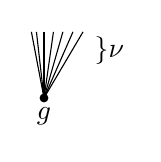
\begin{tikzpicture}[scale=.8]
\fill (0,0) circle(2pt);
\node[below] at (0,0) {$g$};
\foreach \x in {-.2,-.12,0,.15,.3,.46,.62}{\draw (0,0)--(\x,1.05);}
\node[right] at (.65,.75) {$\}\nu$};
\end{tikzpicture}}
toutes ces arêtes (libres) sont de poids 1

et $\mathcal T_{g,\nu}^\pm$ est défini de façon correspondante, via les $(X,\varnothing,\varnothing)$ où $X$ de type $g,\nu$.

\margin{Ça ne suffit pas tout à fait, pour reconstituer les opérations Notamment les opérations
\textcircled{$4^\circ$} (qui \unsure{demande} des \deleted{\unsure{liens}} \inserted{\unsure{``ou''}} \unsure{structures} \unsure{$\mathcal T_{g,\infty}$}) et \textcircled{$5^\circ$}}
\mspage{61}

\scanpage{63}
\mspage{19}
La question essentielle est donc comment reconstituer, pour un graphe \deleted{$\unsure{\Gamma}$} pondéré à
\deleted{à repères donné} \inserted{repères} (disons) $\underline\Gamma$, le
$\mathcal T_{\mathrm{top}}^\pm(\underline\Gamma)$,
\deleted{plus} \inserted{avec} sa dépendance fonctorielle en $\underline\Gamma$,
\deleted{\unsure{des foncteurs des}} \inserted{et l'explicitation}
des sept opérations, à l'exception de $4^\circ)$ et $5^\circ)$.
\margin{\uline{NB} on laisse ici tomber le ``$S$'' ou ``$D$'', contenus déjà dans $\underline\Gamma$.}

Pour l'opération $4^\circ)$, elle sera obtenue automatiquement, par la description explicite des
$\mathcal T_{\mathrm{top}}^\pm(\underline\Gamma)$
(qui sera faite en $=$ temps et de la $=$ façon que pour les $\unsure{S}\mathcal T_{g,\nu}^\pm$ et $\mathcal T_{g,\nu}^\pm$ \unsure{ci-dessus}),
et le bouchage des trous \inserted{pourrait} s'expliciter à l'aide \deleted{\unsure{des 7 opérations}} \inserted{des cas} particuliers de ces opérations pour les
\deleted{analogues des}
$S\mathcal T_{g,\nu}$ et $\mathcal T_{g,\nu}$, qu'il faudrait jeter dans le sac des
\deleted{\unsure{données}} \inserted{structures} ``élémentaires'' à déterminer.

\deleted{$(**)$}\quad
\diagram{\begin{tikzcd}[ampersand replacement=\&,column sep=huge]
\deleted{S}\mathcal T_{g,\nu,\nu'}^\pm\arrow[r]
\&\deleted{S}\mathcal T_{g,\nu-\nu'}
\end{tikzcd}}
\margin{avec ou sans $S$?}
\inserted{les $X\in\operatorname{Ob}\mathcal T_{g,\nu}^\pm$, avec la donnée d'un sous ens. $I'\subset I(X)$ avec $\operatorname{card}I'=\nu'$}
\mspage{62}
\scanpage{64}
\mspage{20}
Mais ces opérations de bouchage sont relativement superficielles, en cela qu'elles ne permettent pas de relier les $\mathcal T_{g,\nu}$, pour $g$ fixé, à des $\mathcal T_{g',\nu'}$ avec $g'<g$. Pour ceci, il faut l'opération \textcircled{$5^\circ$} de gommage des cercles de découpage (= ex-cercles de recollement !).

Néanmoins, il y a, \deleted{une} \inserted{en} liaison avec ça, une autre structure importante à expliciter, c'est celle \deleted{\unsure{des}} des groupoïdes fondamentaux \inserted{$\Pi_1(X;R)$} des $(X,[\unsure{\Sigma}],R)$, \inserted{pour $R\ne\varnothing$,} à base des $R$, (en tant que groupoïdes dépendant fonctoriellement bien sûr de $R$, et \deleted{la donnée} \unsure{comme} \unsure{nouvelle opération}) pour \unsure{tte} \deleted{\unsure{reconstitution}} \inserted{\unsure{représentation}} \unsure{du groupoïde par ens finis}, \unsure{d'un} \inserted{[\unsure{définissant un}]} revêtement \inserted{$X'$} de $X$), d'un nouvel objet du \deleted{$\unsure{\mathcal T_{\mathrm{top}}}$} groupoïde $S\mathcal T_{\mathrm{top}}^\pm$. Déjà dans le cas de $S_1\mathcal T_{0,3}$ la question se pose et est non triviale --- en fait, c'est sans doute là une exigence trop ambitieuse, car

\margin{$\Sigma$ ici est formellement \deleted{\unsure{vide}} vide, \unsure{autant donc} \unsure{pour les mettre dans les} \unsure{cas}, i.e. travailler dans $S\mathcal T_{\mathrm{top}}^\pm$ au lieu de $S\mathcal TD_{\mathrm{top}}^\pm$.}
\mspage{63}
\scanpage{65}
\mspage{21}
elle exigerait d'avoir un ``modèle'' pour $S\mathcal T_{\mathrm{top}}^\pm$ qui soit assez gros pour contenir \inserted{(moyennant déformations)} \uline{toutes les \unsure{cartes|cordes}} --- ça fait un peu gros !

Mais quand même on doit pouvoir sans trop de mal déterminer dans la foulée, avec les modèles qu'on \unsure{désire|cherche}, pour $S\mathcal TD_{\mathrm{top}}^\pm$, des \inserted{modèles des} $\Pi_1(X,R)$, et leur dépendance fonctorielle en $(X,R)$\ldots
\mspage{64}
\scanpage{66}
Découpage de Cartes en ``pantalons'' généralisés
\mspage{65}
\scanpage{67}
Un pantalon \inserted{(topologique)} subdivisé de façon standard, avec un ens $J$ de trous $(\operatorname{card}J=3)$ correspond à un ``triangle pondéré'' i.e.
\[
J\xrightarrow{\pi}\mathbb N
\qquad(\mathrm{NB}\ \pi(\unsure{i|j})=\text{nb d'arêtes qui relient $j$ et $k$, $i\ne j\ne k$})
\]

Carte \inserted{orientée} décomposée pantaloniquement de façon standard $\longleftrightarrow$ \deleted{\unsure{graphe}} squelette pantalonique généralisé

\deleted{i.e. carte \unsure{cellulaire} (\unsure{pas néc. orientée}) dont les sommets marqués sont d'ordre $3$ (\unsure{avec des sommets topologiques} non marqués d'ordre $1$ éventuellement), et avec une pondération des \deleted{\unsure{arêtes orientées}} \inserted{drapeaux} (\unsure{sommet} \inserted{marqué} et arête incidente) de telle façon que l'on ait pour chaque arête (cf ci-contre)}

\figure{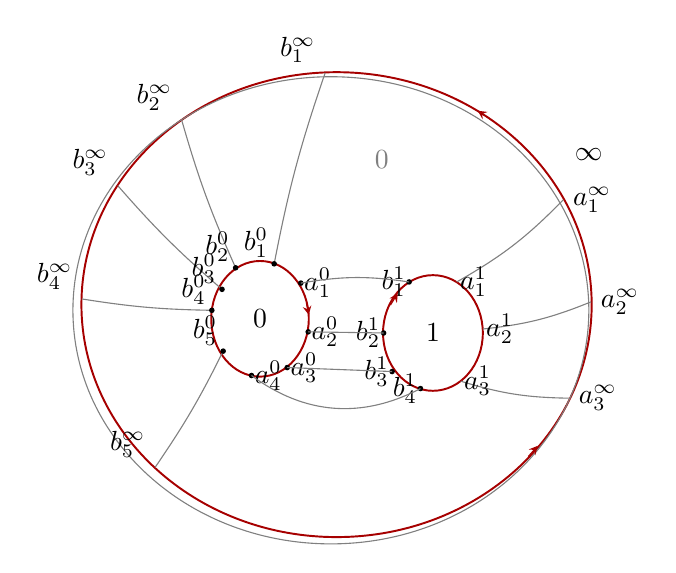
\begin{tikzpicture}[scale=.72,>=stealth]
\draw[red!65!black,line width=.7pt] (0,0) ellipse (4.5 and 4.1);
\draw[gray] (-.1,-.1) ellipse (4.55 and 4.12);
\draw[red!65!black,line width=.7pt] (-1.35,-.25) ellipse (.86 and 1.02);
\draw[red!65!black,line width=.7pt] (1.7,-.5) ellipse (.88 and 1.02);
\node at (-1.35,-.25) {$0$}; \node at (1.7,-.5) {$1$};
\node at (4.45,2.65) {$\infty$}; \node[gray] at (.8,2.55) {$\unsure{0}$};
\coordinate (B01) at (-1.1,.72); \coordinate (B02) at (-1.78,.65);
\coordinate (B03) at (-2.02,.27); \coordinate (B04) at (-2.2,-.1);
\coordinate (B05) at (-2,-.82);
\coordinate (BO1) at (-.2,4.09); \coordinate (BO2) at (-2.73,3.25);
\coordinate (BO3) at (-3.86,2.1); \coordinate (BO4) at (-4.49,.1);
\coordinate (BO5) at (-3.2,-2.87);
\foreach \i in {1,2,3,4,5}{
 \draw[gray] (B0\i) to[bend left=4] (BO\i);
 \fill (B0\i) circle (1.4pt);
 \node[above left,inner sep=2pt] at (B0\i) {$b_{\i}^{0}$};
 \node[above left] at (BO\i) {$b_{\i}^{\infty}$};
}
\coordinate (A01) at (-.63,.38); \coordinate (A02) at (-.5,-.48);
\coordinate (A03) at (-.87,-1.11); \coordinate (A04) at (-1.5,-1.25);
\coordinate (B11) at (1.28,.4); \coordinate (B12) at (.83,-.5);
\coordinate (B13) at (.98,-1.18); \coordinate (B14) at (1.48,-1.48);
\foreach \i in {1,2,3,4}{
 \fill (A0\i) circle (1.4pt); \fill (B1\i) circle (1.4pt);
 \node[right,inner sep=1pt] at (A0\i) {$a_\i^0$};
 \node[left,inner sep=1pt] at (B1\i) {$b_\i^1$};
}
\draw[gray] (A01) to[bend left=9] (B11);
\draw[gray] (A02)--(B12);
\draw[gray] (A03)--(B13);
\draw[gray] (A04) to[bend right=32] (B14);
\coordinate (A11) at (2.12,.4); \coordinate (A12) at (2.58,-.43);
\coordinate (A13) at (2.19,-1.35);
\coordinate (AO1) at (4,1.85); \coordinate (AO2) at (4.49,.05);
\coordinate (AO3) at (4.1,-1.65);
\foreach \i in {1,2,3}{
 \draw[gray] (A1\i) to[bend right=8] (AO\i);
 \node[right,inner sep=1pt] at (A1\i) {$a_\i^1$};
 \node[right] at (AO\i) {$a_\i^\infty$};
}
\draw[->,red!65!black] (-.53,.02)--(-.49,-.18);
\draw[->,red!65!black] (.95,-.01)--(1.08,.2);
\draw[->,red!65!black] (2.7,3.28)--(2.49,3.42);
\draw[->,red!65!black] (3.38,-2.68)--(3.55,-2.49);
\end{tikzpicture}}
% crop-candidate: scan 67



\deleted{\figure{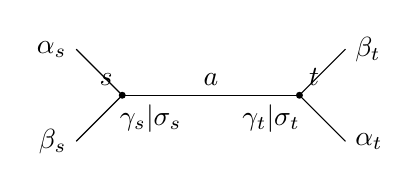
\begin{tikzpicture}[>=stealth,scale=.9]
\fill (0,0) circle (1.4pt) node[above left] {$s$};
\fill (2.5,0) circle (1.4pt) node[above right] {$t$};
\draw (0,0)--(2.5,0) node[midway,above] {$a$};
\draw (0,0)--(-.65,.65) node[left] {$\alpha_s$};
\draw (0,0)--(-.65,-.65) node[left] {$\beta_s$};
\draw (2.5,0)--(3.15,.65) node[right] {$\beta_t$};
\draw (2.5,0)--(3.15,-.65) node[right] {$\alpha_t$};
\node[below] at (.4,0) {$\unsure{\gamma_s|\sigma_s}$};
\node[below] at (2.1,0) {$\unsure{\gamma_t|\sigma_t}$};
\end{tikzpicture}}


\[
\underbrace{\alpha_s+\beta_s}_{\unsure{\gamma'_s|\sigma'_s}}
=
\underbrace{\alpha_t+\beta_t}_{\unsure{\gamma'_t|\sigma'_t}}
\]
et \unsure{=} la \uline{donnée} d'un \deleted{\unsure{isom}} \inserted{anti-}isom des torseurs sous $\unsure{\mathbb Z|\mathbf Z}/\unsure{\gamma|\sigma}$ $(\unsure{\gamma|\sigma}=\unsure{\gamma'_s|\sigma'_s}=\unsure{\gamma'_t|\sigma'_t})$
\[
\substack{\text{somme circulaire}\\\text{de }[1,\alpha_s]\text{ et }[1,\beta_s]}
\ \unsure{\simeq}\
\substack{\text{somme circulaire de}\\{}[1,\alpha_t]\text{ et }[1,\beta_t]}.
\]}

\deleted{\figure{\begin{tikzpicture}[scale=.6]
\coordinate (p) at (1,2); \coordinate (q) at (3,1.3);
\coordinate (r) at (2.7,.1); \coordinate (s) at (1,-.4);
\coordinate (t) at (0,.6);
\draw (p)--(q)--(r)--(s)--(t)--cycle;
\draw (p)--(.8,3.2) (q)--(4.5,1.9) (r)--(3.4,-.7) (s)--(1.1,-1.7) (t)--(-1,-.5);
\fill (r) circle (2pt);
\end{tikzpicture}}

}

\figure{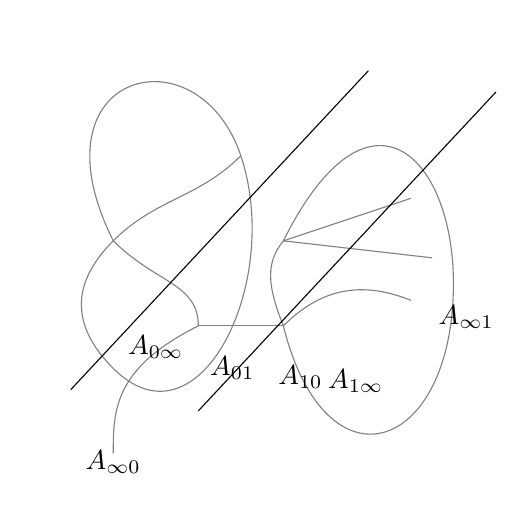
\begin{tikzpicture}[scale=.54,gray]
\draw (-3,1) .. controls (-5,5) and (-1,6) .. (0,3) .. controls (1,0) and (-1,-4) .. (-3,-2) .. controls (-4,-1) and (-4,0) .. (-3,1);
\draw (-3,1) .. controls (-2,2) and (-1,2) .. (0,3);
\draw (-3,1) .. controls (-2,0) and (-1,0) .. (-1,-1);
\draw (-1,-1) .. controls (-3,-2) and (-3,-3) .. (-3,-4);
\draw (1,1) .. controls (3,5) and (5,3) .. (5,0) .. controls (5,-4) and (2,-5) .. (1,-1) .. controls (.6,0) and (.6,.5) .. (1,1);
\draw (1,1)--(4,2);
\draw (1,1)--(4.5,.6);
\draw (1,-1) .. controls (2,0) and (3,0) .. (4,-.4);
\draw (-1,-1)--(1,-1);
\node[black] at (-3,-4.2) {$A_{\infty0}$};
\node[black] at (-2,-1.5) {$A_{0\infty}$};
\node[black] at (-.2,-2) {$A_{01}$};
\node[black] at (1.4,-2.2) {$A_{10}$};
\node[black] at (2.7,-2.3) {$A_{1\infty}$};
\node[black] at (5.3,-.8) {$A_{\infty1}$};
\draw[black] (-4,-2.5)--(3,5);
\draw[black] (-1,-3)--(6,4.5);
\end{tikzpicture}}
% crop-candidate: scan 67



\figure{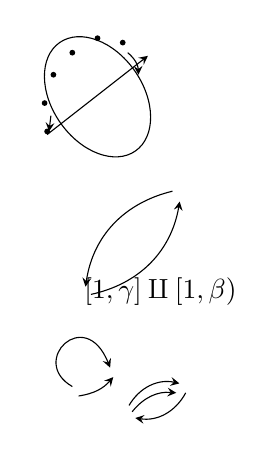
\begin{tikzpicture}[>=stealth,scale=.8]
\draw[rotate=35] (0,0) ellipse (.72 and 1.05);
\draw[->] (-.8,-.6)--(.8,.65);
\foreach \x/\y in {-.8/-.55,-.84/-.1,-.7/.35,-.4/.7,0/.93,.4/.86}
 \fill (\x,\y) circle (1.3pt);
\draw[->] (.48,.7) to[bend left=24] (.65,.35);
\draw[->] (-.74,-.3)--(-.77,-.55);
\begin{scope}[shift={(.6,-2.4)},rotate=35]
\draw[->] (-1,-.2) to[bend right=34] (1,.2);
\draw[->] (1,.4) to[bend right=34] (-1,-.05);
\end{scope}
\node at (1,-3.1) {$\unsure{[1,\gamma]\amalg[1,\beta)}$};
\draw[->] (-.4,-4.6) .. controls (-1.1,-4.2) and (-.2,-3.3) .. (.2,-4.3);
\draw[->] (-.3,-4.75) to[bend right=20] (.25,-4.45);
\draw[->] (.5,-4.9) to[bend left=36] (1.3,-4.55);
\draw[->] (1.4,-4.7) to[bend left=35] (.6,-5.1);
\draw[->] (.55,-5) to[bend left=28] (1.25,-4.7);
\end{tikzpicture}}



\[
\begin{array}{rcl}
\beta+\unsure{\gamma|\sigma}&=&\alpha'\\
\unsure{\gamma|\sigma}+\alpha&=&\beta'\\
\alpha+\beta&=&\unsure{\gamma'|\sigma'}
\end{array}
\qquad
\begin{array}{rcl}
\alpha&=&\dfrac{\beta'+\unsure{\gamma'|\sigma'}-\alpha'}2
=\dfrac{\alpha'+\beta'+\unsure{\gamma'|\sigma'}}2-\alpha'\\[3pt]
\beta&=&\dfrac{\unsure{\gamma'|\sigma'}+\alpha'-\beta'}{\unsure{2}}\\[3pt]
\unsure{\gamma|\sigma}&=&\dfrac{\alpha'+\beta'-\unsure{\gamma'|\sigma'}}2
\end{array}
\]
\[
\unsure{2(\alpha+\beta+\gamma)=\alpha'+\beta'+\gamma'},
\qquad
\unsure{2\alpha+\beta+\gamma=\beta'+\gamma'},
\qquad
\unsure{\beta+\gamma=\alpha'}.
\]
\[
\deleted{\unsure{\alpha}},\quad
\unsure{(\alpha'+\beta'-\gamma')-(\beta+\gamma)},\quad
\unsure{\alpha'},\quad
\unsure{\dfrac{\alpha'+\beta'+\gamma'}2}.
\]

\figure{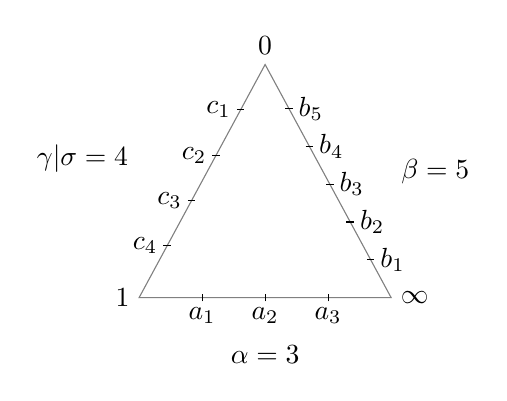
\begin{tikzpicture}[scale=.8]
\draw[gray] (0,0)--(2,3.7)--(4,0)--cycle;
\node[above] at (2,3.7) {$0$}; \node[left] at (0,0) {$1$}; \node[right] at (4,0) {$\infty$};
\foreach \i in {1,2,3} {
 \pgfmathsetmacro{\x}{\i}
 \draw (\x,-.06)--(\x,.06); \node[below] at (\x,0) {$a_\i$};
}
\foreach \i in {1,2,3,4} {
 \pgfmathsetmacro{\y}{3.7-.72*\i}
 \pgfmathsetmacro{\x}{2*\y/3.7}
 \draw (\x-.06,\y)--(\x+.06,\y); \node[left] at (\x,\y) {$c_\i$};
}
\foreach \i in {1,2,3,4,5} {
 \pgfmathsetmacro{\y}{.6*\i}
 \pgfmathsetmacro{\x}{4-2*\y/3.7}
 \draw (\x-.06,\y)--(\x+.06,\y); \node[right] at (\x,\y) {$b_\i$};
}
\node at (-.9,2.2) {$\unsure{\gamma|\sigma}=4$};
\node at (4.7,2) {$\beta=5$};
\node at (2,-.9) {$\alpha=3$};
\end{tikzpicture}}



\figure{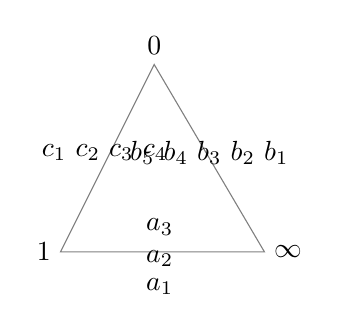
\begin{tikzpicture}[scale=.7]
\draw[gray] (0,0)--(1.7,3.4)--(3.7,0)--cycle;
\node[above] at (1.7,3.4) {$0$}; \node[left] at (0,0) {$1$}; \node[right] at (3.7,0) {$\infty$};
\node at (.8,1.8) {$c_1\ c_2\ c_3\ c_4$};
\node at (2.7,1.8) {$b_5\ b_4\ b_3\ b_2\ b_1$};
\node at (1.8,.45) {$a_3$}; \node at (1.8,-.12) {$a_2$}; \node at (1.8,-.63) {$a_1$};
\end{tikzpicture}}



\figure{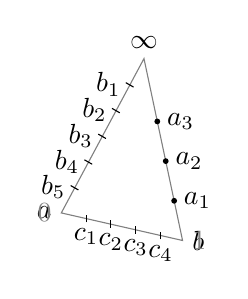
\begin{tikzpicture}[scale=.7]
\draw[gray] (0,0)--(1.5,2.8)--(2.2,-.5)--cycle;
\node[above] at (1.5,2.8) {$\infty$}; \node[left] at (0,0) {$\unsure{a}$}; \node[right] at (2.2,-.5) {$\unsure{b}$};
\node[gray,left] at (0,0) {$0$}; \node[gray,right] at (2.2,-.5) {$1$};
\foreach \i in {1,2,3,4,5} {
 \pgfmathsetmacro{\x}{1.5-.25*\i}
 \pgfmathsetmacro{\y}{2.8-.4667*\i}
 \draw (\x-.08,\y+.03)--(\x+.06,\y-.05); \node[left] at (\x,\y) {$\unsure{b_\i}$};
}
\foreach \i in {1,2,3} {
 \pgfmathsetmacro{\y}{-.5+.72*\i}
 \pgfmathsetmacro{\x}{2.2-.7*(\y+.5)/3.3}
 \fill (\x,\y) circle (1.5pt); \node[right] at (\x,\y) {$\unsure{a_\i}$};
}
\foreach \i in {1,2,3,4} {
 \pgfmathsetmacro{\x}{.45*\i}
 \pgfmathsetmacro{\y}{-.5*\x/2.2}
 \draw (\x,\y-.07)--(\x,\y+.07); \node[below] at (\x,\y) {$\unsure{c_\i}$};
}
\end{tikzpicture}}



\uline{NB} $\alpha',\beta',\unsure{\gamma'|\sigma'}$ \unsure{OK} ssi $\alpha'+\beta'+\unsure{\gamma'|\sigma'}$ pair

\figure{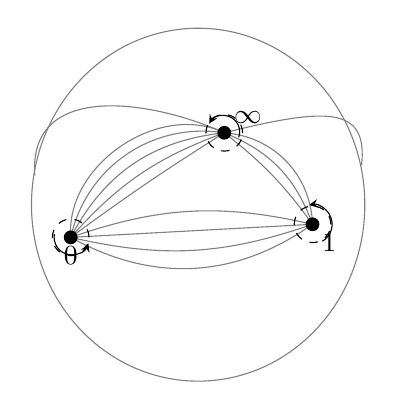
\begin{tikzpicture}[scale=.83,>=stealth]
\draw[gray] (0,0) ellipse (2.55 and 2.7);
\coordinate (z) at (-1.95,-.5); \coordinate (o) at (1.75,-.3); \coordinate (i) at (.4,1.1);
\foreach \b in {16,0,-16,-32} \draw[gray] (z) to[bend left=\b] (o);
\foreach \b in {2,14,28,43,60} \draw[gray] (z) to[bend left=\b] (i);
\foreach \b in {8,24,42} \draw[gray] (i) to[bend left=\b] (o);
\draw[gray] (-2.5,.45) .. controls (-2.6,1.9) and (-.7,1.6) .. (i)
 .. controls (2,1.5) and (2.6,1.5) .. (2.5,.6);
\foreach \p in {z,o,i} {\fill (\p) circle (3pt); \draw[dashed] (\p) circle (.28);}
\node[below] at (z) {$0$}; \node[below right] at (o) {$1$}; \node[above right] at (i) {$\infty$};
\draw[->] (-2.2,-.45) arc (170:340:.27);
\draw[->] (1.9,-.56) arc (-60:100:.3);
\draw[->] (.62,1.03) arc (-20:150:.25);
\end{tikzpicture}}



\[
\begin{array}{l|l}
\text{trois sommets}&\text{sommets d'ordre }\alpha',\beta',\unsure{\gamma'|\sigma'}\\
\alpha+\beta+\unsure{\gamma|\sigma}\ \text{arêtes}&
\end{array}
\]
\deleted{$\unsure{\alpha+\beta+\gamma}$}
\[
\left\{\begin{array}{ll}
(\alpha-1)+(\beta-1)+(\unsure{\gamma|\sigma}-1)&
\overbrace{\text{faces-bigones}}^{=\alpha+\beta+\unsure{\gamma|\sigma}-\unsure{2}}\\
2&\text{faces-triangles}
\end{array}\right.
\quad\bigg|\quad \alpha+\beta+\unsure{\gamma|\sigma}-1\ \text{faces}
\]
\mspage{66}
\scanpage{68}
\figure{\begin{tikzpicture}[scale=.85]
\draw[gray] (0,0) .. controls (-.9,1.5) and (.4,2.2) .. (1.1,1.5) .. controls (2,.9) and (1.2,-.7) .. (0,0);
\draw[gray] (0,0) .. controls (.2,.8) and (1.4,.7) .. (1.1,1.5);
\fill (0,0) circle (2.5pt);
\begin{scope}[shift={(2.8,1.8)}]
\foreach \x in {0,.7,1.4} {\draw (\x,0)--(\x,.35); \fill (\x,0) circle (1.4pt); \fill (\x,.35) circle (1.4pt);}
\foreach \x in {2.1,2.8} {\fill (\x,0) circle (1.1pt); \fill (\x,.35) circle (1.1pt);}
\end{scope}
\end{tikzpicture}}

\figure{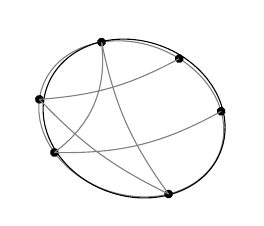
\begin{tikzpicture}[scale=.8]
\begin{scope}[rotate=-20]
\draw[gray] (0,0) ellipse (1.5 and 1.2);
\draw (.04,.02) ellipse (1.47 and 1.23);
\foreach \ang in {30,75,125,190,230,310} {
 \coordinate (p\ang) at ({1.5*cos(\ang)},{1.2*sin(\ang)});
 \fill (p\ang) circle (2pt);
}
\draw[gray] (p125) to[bend right=12] (p310);
\draw[gray] (p75) to[bend left=12] (p190);
\draw[gray] (p30) to[bend left=15] (p230);
\draw[gray] (p190) to[bend right=10] (p310);
\draw[gray] (p125) to[bend left=30] (p230);
\end{scope}
\end{tikzpicture}}

\figure{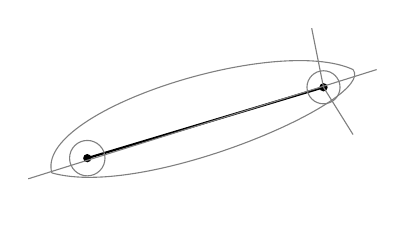
\begin{tikzpicture}[scale=.75]
\fill (0,0) circle (2pt); \fill (4,1.2) circle (2pt);
\draw[thick] (0,0)--(4,1.2);
\draw[gray] (0,0) circle (.3); \draw[gray] (4,1.2) circle (.28);
\draw[gray] (-.6,-.25) .. controls (-.9,.8) and (3.2,2.1) .. (4.5,1.5) .. controls (4.9,1) and (1,-.7) .. (-.6,-.25);
\draw[gray] (-1,-.35)--(4.9,1.5);
\draw[gray] (4,1.2)--(3.8,2.2);
\draw[gray] (4,1.2)--(4.5,.4);
\end{tikzpicture}}

\figure{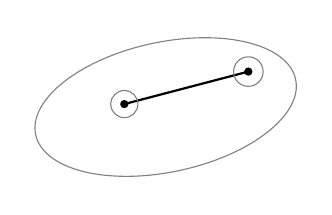
\begin{tikzpicture}[scale=.75]
\draw[gray,rotate=12] (0,0) ellipse (2.25 and 1.1);
\fill (-.7,.05) circle (2pt); \fill (1.4,.6) circle (2pt);
\draw[thick] (-.7,.05)--(1.4,.6);
\draw[gray] (-.7,.05) circle (.23); \draw[gray] (1.4,.6) circle (.25);
\end{tikzpicture}}

\figure{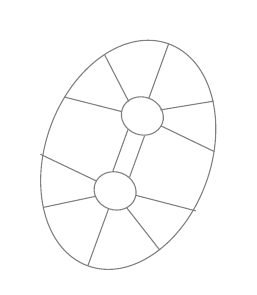
\begin{tikzpicture}[scale=.75,rotate=-20,gray]
\draw (0,0) ellipse (1.4 and 2);
\draw (0,.7) ellipse (.36 and .32);
\draw (0,-.65) ellipse (.36 and .32);
\draw (-.15,-.35)--(-.15,.4) (.15,-.35)--(.15,.4);
\draw (0,1.02)--(0,2);
\draw (-.3,.85)--(-.95,1.45);
\draw (.25,.9)--(1.05,1.35);
\draw (-.36,.65)--(-1.35,.55);
\draw (.36,.65)--(1.35,.55);
\draw (0,-.98)--(0,-2);
\draw (-.28,-.85)--(-1.05,-1.33);
\draw (.28,-.85)--(1.05,-1.33);
\draw (-.36,-.6)--(-1.4,-.5);
\draw (.36,-.6)--(1.4,-.5);
\end{tikzpicture}}
\texttt{****A END JOB 653 PREDONTA\ \ ROOM\ \ 11.24.04 AM 02 JUN 82 R6.PR1\ \ SYS JES2 JOB 653 END A****}

\texttt{****A END JOB 653 PREDONTA\ \ ROOM\ \ 11.24.04 AM 02 JUN 82 R6.PR1\ \ SYS JES2 JOB 653 END A****}

\texttt{****A END JOB 653 PREDONTA\ \ ROOM\ \ 11.24.04 AM 02 JUN 82 R6.PR1\ \ SYS JES2 JOB 653 END A****}

\texttt{****A END JOB 653 PREDONTA\ \ ROOM\ \ 11.24.04 AM 02 JUN 82 R6.PR1\ \ SYS JES2 JOB 653 END A****}

\texttt{****A END JOB 653 PREDONTA\ \ ROOM\ \ 11.24.04 AM 02 JUN 82 R6.PR1\ \ SYS JES2 JOB 653 END A****}

\texttt{****A END JOB 653 PREDONTA\ \ ROOM\ \ 11.24.04 AM 02 JUN 82 R6.PR1\ \ SYS JES2 JOB 653 END A****}
\diagram{\(\begin{array}{llllllll}
\unsure{\texttt{PPPPPPPPPP}} & \unsure{\texttt{RRRRRRRRRR}} & \unsure{\texttt{EEEEEEEEEEEE}} & \unsure{\texttt{DDDDDDDD}} & \unsure{\texttt{OOOOOOOOOOOO}} & \unsure{\texttt{NN\ \ \ \ \ \ \ \ NN}} & \unsure{\texttt{TTTTTTTTTTTT}} & \unsure{\texttt{\ AAAAAAAAAA\ }}\\
\unsure{\texttt{PPPPPPPPPPPP}} & \unsure{\texttt{RRRRRRRRRRRR}} & \unsure{\texttt{EEEEEEEEEEEE}} & \unsure{\texttt{DDDDDDDDDD}} & \unsure{\texttt{OOOOOOOOOOOO}} & \unsure{\texttt{NNN\ \ \ \ \ \ \ NN}} & \unsure{\texttt{TTTTTTTTTTTT}} & \unsure{\texttt{AAAAAAAAAAAA}}\\
\unsure{\texttt{PP\ \ \ \ \ \ \ \ PP}} & \unsure{\texttt{RR\ \ \ \ \ \ \ \ RR}} & \unsure{\texttt{EE}} & \unsure{\texttt{DD\ \ \ \ \ \ \ \ DD}} & \unsure{\texttt{OO\ \ \ \ \ \ \ \ OO}} & \unsure{\texttt{NNNN\ \ \ \ \ \ NN}} & \unsure{\texttt{\ \ \ \ \ TT\ \ \ \ \ }} & \unsure{\texttt{AA\ \ \ \ \ \ \ \ AA}}\\
\unsure{\texttt{PP\ \ \ \ \ \ \ \ PP}} & \unsure{\texttt{RR\ \ \ \ \ \ \ \ RR}} & \unsure{\texttt{EE}} & \unsure{\texttt{DD\ \ \ \ \ \ \ \ DD}} & \unsure{\texttt{OO\ \ \ \ \ \ \ \ OO}} & \unsure{\texttt{NN\ NN\ \ \ \ \ NN}} & \unsure{\texttt{\ \ \ \ \ TT\ \ \ \ \ }} & \unsure{\texttt{AA\ \ \ \ \ \ \ \ AA}}\\
\unsure{\texttt{PP\ \ \ \ \ \ \ \ PP}} & \unsure{\texttt{RR\ \ \ \ \ \ \ \ RR}} & \unsure{\texttt{EE}} & \unsure{\texttt{DD\ \ \ \ \ \ \ \ DD}} & \unsure{\texttt{OO\ \ \ \ \ \ \ \ OO}} & \unsure{\texttt{NN\ \ NN\ \ \ \ NN}} & \unsure{\texttt{\ \ \ \ \ TT\ \ \ \ \ }} & \unsure{\texttt{AA\ \ \ \ \ \ \ \ AA}}\\
\unsure{\texttt{PPPPPPPPPPPP}} & \unsure{\texttt{RRRRRRRRRRRR}} & \unsure{\texttt{EEEEEEE}} & \unsure{\texttt{DD\ \ \ \ \ \ \ \ DD}} & \unsure{\texttt{OO\ \ \ \ \ \ \ \ OO}} & \unsure{\texttt{NN\ \ \ NN\ \ \ NN}} & \unsure{\texttt{\ \ \ \ \ TT\ \ \ \ \ }} & \unsure{\texttt{AAAAAAAAAAAA}}\\
\unsure{\texttt{PPPPPPPPPP}} & \unsure{\texttt{RRRRRRRRRR}} & \unsure{\texttt{EEEEEEE}} & \unsure{\texttt{DD\ \ \ \ \ \ \ \ DD}} & \unsure{\texttt{OO\ \ \ \ \ \ \ \ OO}} & \unsure{\texttt{NN\ \ \ \ NN\ \ NN}} & \unsure{\texttt{\ \ \ \ \ TT\ \ \ \ \ }} & \unsure{\texttt{AAAAAAAAAAAA}}\\
\unsure{\texttt{PP}} & \unsure{\texttt{RR\ \ \ RR}} & \unsure{\texttt{EE}} & \unsure{\texttt{DD\ \ \ \ \ \ \ \ DD}} & \unsure{\texttt{OO\ \ \ \ \ \ \ \ OO}} & \unsure{\texttt{NN\ \ \ \ \ NN\ NN}} & \unsure{\texttt{\ \ \ \ \ TT\ \ \ \ \ }} & \unsure{\texttt{AA\ \ \ \ \ \ \ \ AA}}\\
\unsure{\texttt{PP}} & \unsure{\texttt{RR\ \ \ \ RR}} & \unsure{\texttt{EE}} & \unsure{\texttt{DD\ \ \ \ \ \ \ \ DD}} & \unsure{\texttt{OO\ \ \ \ \ \ \ \ OO}} & \unsure{\texttt{NN\ \ \ \ \ \ NNNN}} & \unsure{\texttt{\ \ \ \ \ TT\ \ \ \ \ }} & \unsure{\texttt{AA\ \ \ \ \ \ \ \ AA}}\\
\unsure{\texttt{PP}} & \unsure{\texttt{RR\ \ \ \ \ RR}} & \unsure{\texttt{EE}} & \unsure{\texttt{DD\ \ \ \ \ \ \ \ DD}} & \unsure{\texttt{OO\ \ \ \ \ \ \ \ OO}} & \unsure{\texttt{NN\ \ \ \ \ \ \ NNN}} & \unsure{\texttt{\ \ \ \ \ TT\ \ \ \ \ }} & \unsure{\texttt{AA\ \ \ \ \ \ \ \ AA}}\\
\unsure{\texttt{PP}} & \unsure{\texttt{RR\ \ \ \ \ \ RR}} & \unsure{\texttt{EEEEEEEEEEEE}} & \unsure{\texttt{DDDDDDDDDD}} & \unsure{\texttt{OOOOOOOOOOOO}} & \unsure{\texttt{NN\ \ \ \ \ \ \ \ NN}} & \unsure{\texttt{\ \ \ \ \ TT\ \ \ \ \ }} & \unsure{\texttt{AA\ \ \ \ \ \ \ \ AA}}\\
\unsure{\texttt{PP}} & \unsure{\texttt{RR\ \ \ \ \ \ \ \ RR}} & \unsure{\texttt{EEEEEEEEEEEE}} & \unsure{\texttt{DDDDDDDD}} & \unsure{\texttt{OOOOOOOOOOOO}} & \unsure{\texttt{NN\ \ \ \ \ \ \ \ \ N}} & \unsure{\texttt{\ \ \ \ \ TT\ \ \ \ \ }} & \unsure{\texttt{AA\ \ \ \ \ \ \ \ AA}}\\
\end{array}\)}
\diagram{\(\begin{array}{llll}
\unsure{\texttt{\ \ \ \ 00000000}} & \unsure{\texttt{\ \ \ \ 00000000}} & \unsure{\texttt{\ \ \ \ 00000000}} & \unsure{\texttt{\ \ \ \ 00000000}}\\
\unsure{\texttt{\ \ \ 0000000000}} & \unsure{\texttt{\ \ \ 0000000000}} & \unsure{\texttt{\ \ \ 0000000000}} & \unsure{\texttt{\ \ \ 0000000000}}\\
\unsure{\texttt{\ \ 00\ \ \ \ \ \ 0000}} & \unsure{\texttt{\ \ 00\ \ \ \ \ \ 0000}} & \unsure{\texttt{\ \ 00\ \ \ \ \ \ 0000}} & \unsure{\texttt{\ \ 00\ \ \ \ \ \ 0000}}\\
\unsure{\texttt{\ 00\ \ \ \ \ \ 00\ 00}} & \unsure{\texttt{\ 00\ \ \ \ \ \ 00\ 00}} & \unsure{\texttt{\ 00\ \ \ \ \ \ 00\ 00}} & \unsure{\texttt{\ 00\ \ \ \ \ \ 00\ 00}}\\
\unsure{\texttt{00\ \ \ \ \ \ 00\ \ 00}} & \unsure{\texttt{00\ \ \ \ \ \ 00\ \ 00}} & \unsure{\texttt{00\ \ \ \ \ \ 00\ \ 00}} & \unsure{\texttt{00\ \ \ \ \ \ 00\ \ 00}}\\
\unsure{\texttt{00\ \ \ \ 00\ \ \ \ 00}} & \unsure{\texttt{00\ \ \ \ 00\ \ \ \ 00}} & \unsure{\texttt{00\ \ \ \ 00\ \ \ \ 00}} & \unsure{\texttt{00\ \ \ \ 00\ \ \ \ 00}}\\
\unsure{\texttt{00\ \ \ 00\ \ \ \ \ 00}} & \unsure{\texttt{00\ \ \ 00\ \ \ \ \ 00}} & \unsure{\texttt{00\ \ \ 00\ \ \ \ \ 00}} & \unsure{\texttt{00\ \ \ 00\ \ \ \ \ 00}}\\
\unsure{\texttt{00\ \ 00\ \ \ \ \ \ 00}} & \unsure{\texttt{00\ \ 00\ \ \ \ \ \ 00}} & \unsure{\texttt{00\ \ 00\ \ \ \ \ \ 00}} & \unsure{\texttt{00\ \ 00\ \ \ \ \ \ 00}}\\
\unsure{\texttt{00\ 00\ \ \ \ \ \ \ 00}} & \unsure{\texttt{00\ 00\ \ \ \ \ \ \ 00}} & \unsure{\texttt{00\ 00\ \ \ \ \ \ \ 00}} & \unsure{\texttt{00\ 00\ \ \ \ \ \ \ 00}}\\
\unsure{\texttt{000\ \ \ \ \ \ \ \ \ 00}} & \unsure{\texttt{000\ \ \ \ \ \ \ \ \ 00}} & \unsure{\texttt{000\ \ \ \ \ \ \ \ \ 00}} & \unsure{\texttt{000\ \ \ \ \ \ \ \ \ 00}}\\
\unsure{\texttt{0000000000}} & \unsure{\texttt{0000000000}} & \unsure{\texttt{0000000000}} & \unsure{\texttt{0000000000}}\\
\unsure{\texttt{00000000}} & \unsure{\texttt{00000000}} & \unsure{\texttt{00000000}} & \unsure{\texttt{00000000}}\\
\end{array}\)}
\mspage{67}
\scanpage{69}
\figure{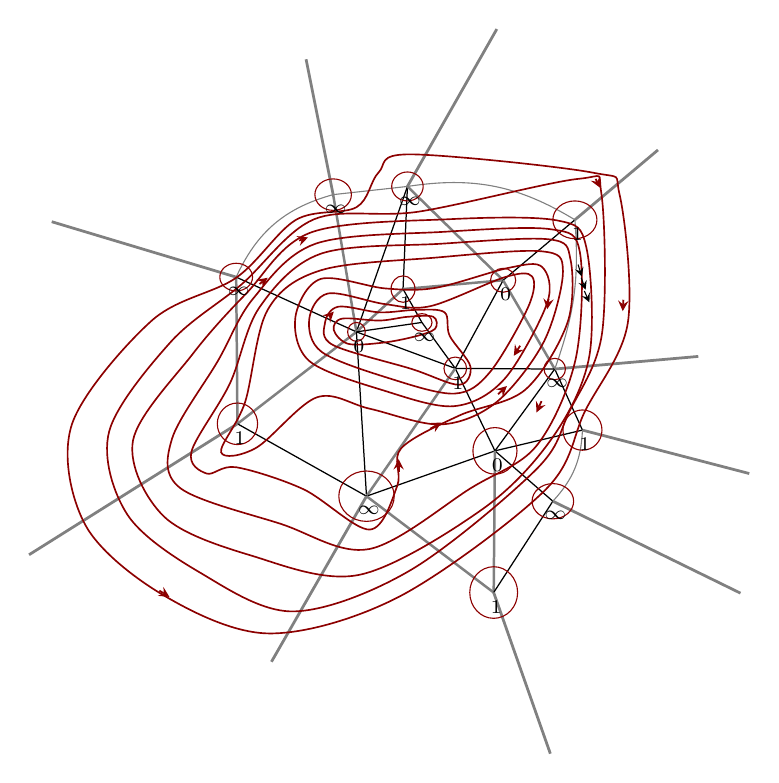
\begin{tikzpicture}[x=.008cm,y=-.008cm,>=stealth]
\coordinate (a) at (878,350);
\coordinate (b) at (996,337);
\coordinate (c) at (1262,390);
\coordinate (d) at (724,481);
\coordinate (e) at (989,500);
\coordinate (f) at (915,568);
\coordinate (g) at (1019,553);
\coordinate (h) at (1148,486);
\coordinate (i) at (1072,626);
\coordinate (j) at (1230,627);
\coordinate (k) at (726,714);
\coordinate (l) at (931,829);
\coordinate (m) at (1135,757);
\coordinate (n) at (1274,724);
\coordinate (o) at (1227,837);
\coordinate (p) at (1133,982);
\draw[gray,line width=.9pt] (f)--(a);
\draw[black,line width=.45pt] (f)--(b);
\draw[black,line width=.45pt] (f)--(d);
\draw[gray,line width=.9pt] (f)--(e);
\draw[black,line width=.45pt] (f)--(g);
\draw[black,line width=.45pt] (f)--(i);
\draw[gray,line width=.9pt] (f)--(k);
\draw[black,line width=.45pt] (f)--(l);
\draw[black,line width=.45pt] (b)--(e);
\draw[gray,line width=.9pt] (e)--(h);
\draw[black,line width=.45pt] (e)--(g);
\draw[black,line width=.45pt] (g)--(i);
\draw[gray,line width=.9pt] (b)--(h);
\draw[black,line width=.45pt] (c)--(h);
\draw[black,line width=.45pt] (h)--(i);
\draw[gray,line width=.9pt] (h)--(j);
\draw[black,line width=.45pt] (i)--(j);
\draw[black,line width=.45pt] (i)--(m);
\draw[gray,line width=.9pt] (i)--(l);
\draw[black,line width=.45pt] (j)--(m);
\draw[black,line width=.45pt] (j)--(n);
\draw[gray,line width=.9pt] (d)--(k);
\draw[black,line width=.45pt] (k)--(l);
\draw[black,line width=.45pt] (l)--(m);
\draw[gray,line width=.9pt] (l)--(p);
\draw[black,line width=.45pt] (m)--(n);
\draw[black,line width=.45pt] (m)--(o);
\draw[gray,line width=.9pt] (m)--(p);
\draw[black,line width=.45pt] (o)--(p);
\draw[gray] (a) to[bend right=25] (d);
\draw[gray] (a)--(b);
\draw[gray] (b) to[bend left=20] (c);
\draw[gray] (c) to[bend left=12] (j);
\draw[gray] (n) to[bend left=20] (o);
\draw[gray,line width=1pt] (a)--(835,135);
\draw[gray,line width=1pt] (b)--(1138,87);
\draw[gray,line width=1pt] (c)--(1394,279);
\draw[gray,line width=1pt] (d)--(431,393);
\draw[gray,line width=1pt] (j)--(1458,607);
\draw[gray,line width=1pt] (k)--(395,922);
\draw[gray,line width=1pt] (l)--(780,1092);
\draw[gray,line width=1pt] (n)--(1539,793);
\draw[gray,line width=1pt] (o)--(1525,983);
\draw[gray,line width=1pt] (p)--(1223,1238);
\draw[red!55!black,line width=.6pt] plot[smooth cycle,tension=.55] coordinates {(724,482) (590,550) (463,715) (484,874) (608,986) (777,1047) (984,988) (1215,819) (1278,694) (1346,554) (1333,350) (1290,315) (1000,286) (950,315) (915,370) (819,390)};
\draw[red!55!black,line width=.6pt] plot[smooth cycle,tension=.55] coordinates {(732,493) (620,584) (522,727) (551,858) (666,950) (814,1012) (1000,947) (1200,787) (1253,695) (1305,571) (1304,348) (1267,325) (1014,377) (848,389)};
\draw[red!55!black,line width=.6pt] plot[smooth cycle,tension=.55] coordinates {(740,507) (655,603) (560,741) (609,861) (747,923) (919,954) (1116,849) (1227,735) (1285,606) (1280,433) (1234,391) (1063,389) (843,410)};
\draw[red!55!black,line width=.6pt] plot[smooth cycle,tension=.55] coordinates {(751,515) (695,614) (622,738) (635,816) (795,873) (935,913) (1097,816) (1201,749) (1263,612) (1270,442) (1224,405) (1055,409) (850,428)};
\draw[red!55!black,line width=.6pt] plot[smooth cycle,tension=.55] coordinates {(761,529) (714,650) (653,758) (677,793) (724,783) (831,818) (936,882) (980,812) (986,753) (1078,701) (1183,660) (1250,554) (1255,453) (1221,421) (1049,428) (858,444)};
\draw[red!55!black,line width=.6pt] plot[smooth cycle,tension=.55] coordinates {(774,533) (738,680) (700,759) (756,752) (852,672) (936,690) (1049,715) (1137,680) (1213,583) (1243,471) (1209,440) (1041,450) (859,470)};
\draw[red!55!black,line width=.6pt] plot[smooth cycle,tension=.55] coordinates {(858,484) (818,545) (841,615) (958,661) (1070,686) (1150,643) (1218,522) (1210,465) (1158,466) (1041,498) (961,499)};
\draw[red!55!black,line width=.6pt] plot[smooth cycle,tension=.55] coordinates {(870,507) (840,548) (860,600) (968,642) (1071,666) (1127,632) (1188,528) (1194,480) (1151,481) (1033,527) (961,524)};
\draw[red!55!black,line width=.6pt] plot[smooth cycle,tension=.55] coordinates {(886,528) (865,554) (878,589) (1003,627) (1078,652) (1096,623) (1063,574) (1055,537) (1010,533) (952,537)};
\draw[red!55!black,line width=.6pt] plot[smooth cycle,tension=.55] coordinates {(892,547) (879,565) (902,587) (958,585) (1009,575) (1040,563) (1037,544) (997,544) (952,550)};
\draw[red!55!black] (a) ellipse (29 and 25);
\draw[red!55!black] (b) ellipse (25 and 23);
\draw[red!55!black] (c) ellipse (35 and 30);
\draw[red!55!black] (d) ellipse (26 and 22);
\draw[red!55!black] (e) ellipse (19 and 21);
\draw[red!55!black] (f) ellipse (14 and 15);
\draw[red!55!black] (g) ellipse (16 and 14);
\draw[red!55!black] (h) ellipse (20 and 19);
\draw[red!55!black] (i) ellipse (18 and 18);
\draw[red!55!black] (j) ellipse (17 and 17);
\draw[red!55!black] (k) ellipse (32 and 33);
\draw[red!55!black] (l) ellipse (44 and 40);
\draw[red!55!black] (m) ellipse (35 and 37);
\draw[red!55!black] (n) ellipse (31 and 32);
\draw[red!55!black] (o) ellipse (33 and 28);
\draw[red!55!black] (p) ellipse (38 and 41);
\node[font=\scriptsize,inner sep=0pt] at (882,373) {$\unsure{\infty}$};
\node[font=\scriptsize,inner sep=0pt] at (1000,360) {$\unsure{\infty}$};
\node[font=\scriptsize,inner sep=0pt] at (1266,413) {$1$};
\node[font=\scriptsize,inner sep=0pt] at (728,504) {$\unsure{\infty}$};
\node[font=\scriptsize,inner sep=0pt] at (993,523) {$\unsure{1}$};
\node[font=\scriptsize,inner sep=0pt] at (919,591) {$0$};
\node[font=\scriptsize,inner sep=0pt] at (1023,576) {$\infty$};
\node[font=\scriptsize,inner sep=0pt] at (1152,509) {$0$};
\node[font=\scriptsize,inner sep=0pt] at (1076,649) {$1$};
\node[font=\scriptsize,inner sep=0pt] at (1234,650) {$\infty$};
\node[font=\scriptsize,inner sep=0pt] at (730,737) {$1$};
\node[font=\scriptsize,inner sep=0pt] at (935,852) {$\infty$};
\node[font=\scriptsize,inner sep=0pt] at (1139,780) {$0$};
\node[font=\scriptsize,inner sep=0pt] at (1278,747) {$1$};
\node[font=\scriptsize,inner sep=0pt] at (1231,860) {$\infty$};
\node[font=\scriptsize,inner sep=0pt] at (1137,1005) {$1$};
\draw[->,red!55!black,line width=.65pt] (602,979)--(618,989);
\draw[->,red!55!black,line width=.65pt] (1295,325)--(1302,339);
\draw[->,red!55!black,line width=.65pt] (1339,517)--(1338,535);
\draw[->,red!55!black,line width=.65pt] (1209,678)--(1201,696);
\draw[->,red!55!black,line width=.65pt] (982,791)--(982,770);
\draw[->,red!55!black,line width=.65pt] (1032,722)--(1050,712);
\draw[->,red!55!black,line width=.65pt] (873,542)--(879,536);
\draw[->,red!55!black,line width=.65pt] (761,492)--(774,482);
\draw[->,red!55!black,line width=.65pt] (824,423)--(838,418);
\draw[->,red!55!black,line width=.65pt] (1175,590)--(1165,606);
\draw[->,red!55!black,line width=.65pt] (1220,516)--(1218,532);
\draw[->,red!55!black,line width=.65pt] (1140,667)--(1154,654);
\draw[->,black] (1272,482)--(1279,501);
\draw[->,black] (1277,503)--(1285,521);
\draw[->,black] (1267,461)--(1273,480);
\end{tikzpicture}}
% crop-candidate: scan 69


\mspage{68}
\scanpage{70}
\figure{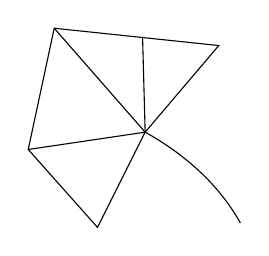
\begin{tikzpicture}[scale=1.1]
\draw (0,0)--(.3,1.4)--(2.2,1.2)--(1.35,.2)--(.8,-.9)--cycle;
\draw (.3,1.4)--(1.35,.2)--(0,0);
\draw (1.35,.2)--(1.32,1.3);
\draw (1.35,.2) .. controls (1.8,-.05) and (2.2,-.4) .. (2.45,-.85);
\end{tikzpicture}}
\figure{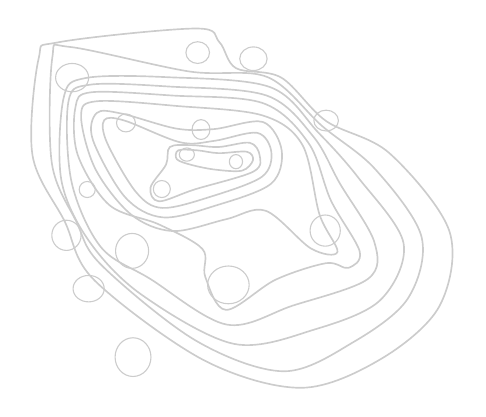
\begin{tikzpicture}[x=-.006cm,y=-.006cm]
\coordinate (a) at (878,350);
\coordinate (b) at (996,337);
\coordinate (c) at (1262,390);
\coordinate (d) at (724,481);
\coordinate (e) at (989,500);
\coordinate (f) at (915,568);
\coordinate (g) at (1019,553);
\coordinate (h) at (1148,486);
\coordinate (i) at (1072,626);
\coordinate (j) at (1230,627);
\coordinate (k) at (726,714);
\coordinate (l) at (931,829);
\coordinate (m) at (1135,757);
\coordinate (n) at (1274,724);
\coordinate (o) at (1227,837);
\coordinate (p) at (1133,982);
\draw[gray!40,line width=.6pt] plot[smooth cycle,tension=.55] coordinates {(724,482) (590,550) (463,715) (484,874) (608,986) (777,1047) (984,988) (1215,819) (1278,694) (1346,554) (1333,350) (1290,315) (1000,286) (950,315) (915,370) (819,390)};
\draw[gray!40,line width=.6pt] plot[smooth cycle,tension=.55] coordinates {(732,493) (620,584) (522,727) (551,858) (666,950) (814,1012) (1000,947) (1200,787) (1253,695) (1305,571) (1304,348) (1267,325) (1014,377) (848,389)};
\draw[gray!40,line width=.6pt] plot[smooth cycle,tension=.55] coordinates {(740,507) (655,603) (560,741) (609,861) (747,923) (919,954) (1116,849) (1227,735) (1285,606) (1280,433) (1234,391) (1063,389) (843,410)};
\draw[gray!40,line width=.6pt] plot[smooth cycle,tension=.55] coordinates {(751,515) (695,614) (622,738) (635,816) (795,873) (935,913) (1097,816) (1201,749) (1263,612) (1270,442) (1224,405) (1055,409) (850,428)};
\draw[gray!40,line width=.6pt] plot[smooth cycle,tension=.55] coordinates {(761,529) (714,650) (653,758) (677,793) (724,783) (831,818) (936,882) (980,812) (986,753) (1078,701) (1183,660) (1250,554) (1255,453) (1221,421) (1049,428) (858,444)};
\draw[gray!40,line width=.6pt] plot[smooth cycle,tension=.55] coordinates {(774,533) (738,680) (700,759) (756,752) (852,672) (936,690) (1049,715) (1137,680) (1213,583) (1243,471) (1209,440) (1041,450) (859,470)};
\draw[gray!40,line width=.6pt] plot[smooth cycle,tension=.55] coordinates {(858,484) (818,545) (841,615) (958,661) (1070,686) (1150,643) (1218,522) (1210,465) (1158,466) (1041,498) (961,499)};
\draw[gray!40,line width=.6pt] plot[smooth cycle,tension=.55] coordinates {(870,507) (840,548) (860,600) (968,642) (1071,666) (1127,632) (1188,528) (1194,480) (1151,481) (1033,527) (961,524)};
\draw[gray!40,line width=.6pt] plot[smooth cycle,tension=.55] coordinates {(886,528) (865,554) (878,589) (1003,627) (1078,652) (1096,623) (1063,574) (1055,537) (1010,533) (952,537)};
\draw[gray!40,line width=.6pt] plot[smooth cycle,tension=.55] coordinates {(892,547) (879,565) (902,587) (958,585) (1009,575) (1040,563) (1037,544) (997,544) (952,550)};
\draw[gray!40] (a) ellipse (29 and 25);
\draw[gray!40] (b) ellipse (25 and 23);
\draw[gray!40] (c) ellipse (35 and 30);
\draw[gray!40] (d) ellipse (26 and 22);
\draw[gray!40] (e) ellipse (19 and 21);
\draw[gray!40] (f) ellipse (14 and 15);
\draw[gray!40] (g) ellipse (16 and 14);
\draw[gray!40] (h) ellipse (20 and 19);
\draw[gray!40] (i) ellipse (18 and 18);
\draw[gray!40] (j) ellipse (17 and 17);
\draw[gray!40] (k) ellipse (32 and 33);
\draw[gray!40] (l) ellipse (44 and 40);
\draw[gray!40] (m) ellipse (35 and 37);
\draw[gray!40] (n) ellipse (31 and 32);
\draw[gray!40] (o) ellipse (33 and 28);
\draw[gray!40] (p) ellipse (38 and 41);
\end{tikzpicture}}

\deleted{\diagram{\begin{tikzcd}[ampersand replacement=\&,row sep=large,column sep=huge]
{[\pm1]} \& {[\pm1]}\\
\mathcal T_{\mathrm{top}}^\pm \arrow[u] \arrow[r,hook,"\mathrm{imm}"]
 \& \unsure{S\mathcal TS_{\mathrm{top}}^\pm} \arrow[u]\\
\mathcal T_{\mathrm{top}} \arrow[u,"\text{fid ess. surj.}"] \arrow[r,hook,"\mathrm{imm}"]
 \& \mathcal TS_{\mathrm{top}} \arrow[u,"\text{fid ess. surj.}"']
\end{tikzcd}}}

\deleted{On a
\[
\pi_0(\mathcal T_{\mathrm{top}})
\xrightarrow{\sim}\pi_0(\mathcal T_{\mathrm{top}}^\pm)\simeq
\]}
\mspage{69}
\scanpage{71}
Groupoïdes de \uline{Teichmüller}

1) Groupoïdes topologiques $\boxed{S\mathcal T_{\mathrm{top}}}$.
(\uline{groupoïde de Teichmüller spécial orienté topologique})

Objets : paires $(X,S)$
\[
\left|\begin{array}{l}
X\ \text{surface à bord compacte \uline{orientée}}\\
S\subset\partial X\quad\text{partie finie du bord}
\end{array}\right.
\]
Morphismes $(X,S)\longrightarrow(X',S')$ : classes d'isotopie d'isomorphismes

\deleted{\unsure{Trois}} \uline{Variantes}

$1^\circ)$ $S=\varnothing$ on écrit $\mathcal T_{\mathrm{top}}$ sous-groupoïde ouvert.
(\uline{groupoïde de T. \deleted{\unsure{orient}} orienté topologique})

$2^\circ)$ $\boxed{S\mathcal T_{\mathrm{top}}^\pm}$ mêmes objets, mais plus de flèches :
classes d'isotopie d'homéom. $(X,S)\xrightarrow{\sim}(X',S')$, ne respectant pas l'orientation nécessairement.

On a
\diagram{\begin{tikzcd}[ampersand replacement=\&,column sep=large]
S\mathcal T_{\mathrm{top}}^\pm \arrow[r,"\unsure{\chi}","\text{(signature)}"']
\& \deleted{\unsure{\mathfrak G}}\ \substack{\text{groupoïde \deleted{ponctuel}}\\
\text{défini par le groupe}\\
\pm1,\ \text{noté }[\pm1]}
\end{tikzcd}}
\unsure{le|la} \deleted{noyau} \deleted{est} (la catégorie fibre) est $S\mathcal T_{\mathrm{top}}$

$2^\circ)$ $(X,\Sigma,S)$, avec
\[
\left|\begin{array}{l}
X\ \text{compacte à bord orienté}\\
\Sigma\ \text{sous-variété \deleted{fermée} \inserted{compacte} de dim $1$}\\
\qquad\text{de }X\setminus\partial X\\
S\subset\Sigma\cup\partial X\quad\text{partie finie}
\end{array}\right.
\]
morphismes : classes d'isotopie d'homéom respectant l'orientation.
Notation $\mathcal T\deleted{\unsure{S}}\inserted{D}_{\mathrm{top}}$
($D$ initiale de dévissage \deleted{``\unsure{sauvage}''}) :
``\uline{groupoïde de Teichmüller orienté dévissé topologique}''.

\uline{NB}
\[
S\mathcal T_{\mathrm{top}}\subset S\mathcal TD_{\mathrm{top}}
\qquad
\substack{\text{imm. ouverte}\\(\deleted{\text{immersion pleine}})}
\]
\[
\substack{\Vert\\\text{sous groupoïde des objets tels que }\Sigma=\varnothing}
\]

$3^\circ)$ On définit de $=$ $\unsure{\mathcal TS_{\mathrm{top}}^\pm}$
(\uline{groupoïde de Teichmüller bi-orienté dévissé topologique})
\figure{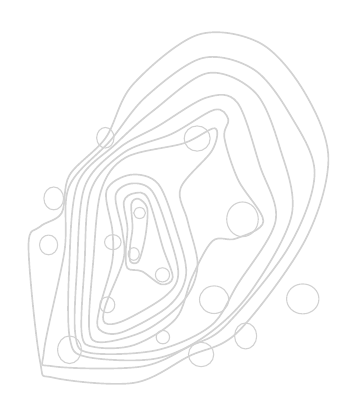
\begin{tikzpicture}[x=-.005cm,y=-.005cm,rotate=90]
\coordinate (a) at (878,350);
\coordinate (b) at (996,337);
\coordinate (c) at (1262,390);
\coordinate (d) at (724,481);
\coordinate (e) at (989,500);
\coordinate (f) at (915,568);
\coordinate (g) at (1019,553);
\coordinate (h) at (1148,486);
\coordinate (i) at (1072,626);
\coordinate (j) at (1230,627);
\coordinate (k) at (726,714);
\coordinate (l) at (931,829);
\coordinate (m) at (1135,757);
\coordinate (n) at (1274,724);
\coordinate (o) at (1227,837);
\coordinate (p) at (1133,982);
\draw[gray!35,line width=.6pt] plot[smooth cycle,tension=.55] coordinates {(724,482) (590,550) (463,715) (484,874) (608,986) (777,1047) (984,988) (1215,819) (1278,694) (1346,554) (1333,350) (1290,315) (1000,286) (950,315) (915,370) (819,390)};
\draw[gray!35,line width=.6pt] plot[smooth cycle,tension=.55] coordinates {(732,493) (620,584) (522,727) (551,858) (666,950) (814,1012) (1000,947) (1200,787) (1253,695) (1305,571) (1304,348) (1267,325) (1014,377) (848,389)};
\draw[gray!35,line width=.6pt] plot[smooth cycle,tension=.55] coordinates {(740,507) (655,603) (560,741) (609,861) (747,923) (919,954) (1116,849) (1227,735) (1285,606) (1280,433) (1234,391) (1063,389) (843,410)};
\draw[gray!35,line width=.6pt] plot[smooth cycle,tension=.55] coordinates {(751,515) (695,614) (622,738) (635,816) (795,873) (935,913) (1097,816) (1201,749) (1263,612) (1270,442) (1224,405) (1055,409) (850,428)};
\draw[gray!35,line width=.6pt] plot[smooth cycle,tension=.55] coordinates {(761,529) (714,650) (653,758) (677,793) (724,783) (831,818) (936,882) (980,812) (986,753) (1078,701) (1183,660) (1250,554) (1255,453) (1221,421) (1049,428) (858,444)};
\draw[gray!35,line width=.6pt] plot[smooth cycle,tension=.55] coordinates {(774,533) (738,680) (700,759) (756,752) (852,672) (936,690) (1049,715) (1137,680) (1213,583) (1243,471) (1209,440) (1041,450) (859,470)};
\draw[gray!35,line width=.6pt] plot[smooth cycle,tension=.55] coordinates {(858,484) (818,545) (841,615) (958,661) (1070,686) (1150,643) (1218,522) (1210,465) (1158,466) (1041,498) (961,499)};
\draw[gray!35,line width=.6pt] plot[smooth cycle,tension=.55] coordinates {(870,507) (840,548) (860,600) (968,642) (1071,666) (1127,632) (1188,528) (1194,480) (1151,481) (1033,527) (961,524)};
\draw[gray!35,line width=.6pt] plot[smooth cycle,tension=.55] coordinates {(886,528) (865,554) (878,589) (1003,627) (1078,652) (1096,623) (1063,574) (1055,537) (1010,533) (952,537)};
\draw[gray!35,line width=.6pt] plot[smooth cycle,tension=.55] coordinates {(892,547) (879,565) (902,587) (958,585) (1009,575) (1040,563) (1037,544) (997,544) (952,550)};
\draw[gray!35] (a) ellipse (29 and 25);
\draw[gray!35] (b) ellipse (25 and 23);
\draw[gray!35] (c) ellipse (35 and 30);
\draw[gray!35] (d) ellipse (26 and 22);
\draw[gray!35] (e) ellipse (19 and 21);
\draw[gray!35] (f) ellipse (14 and 15);
\draw[gray!35] (g) ellipse (16 and 14);
\draw[gray!35] (h) ellipse (20 and 19);
\draw[gray!35] (i) ellipse (18 and 18);
\draw[gray!35] (j) ellipse (17 and 17);
\draw[gray!35] (k) ellipse (32 and 33);
\draw[gray!35] (l) ellipse (44 and 40);
\draw[gray!35] (m) ellipse (35 and 37);
\draw[gray!35] (n) ellipse (31 and 32);
\draw[gray!35] (o) ellipse (33 and 28);
\draw[gray!35] (p) ellipse (38 and 41);\end{tikzpicture}}
\mspage{70}
\scanpage{72}
découpage pantalonique d'une carte (triangulée)

\figure{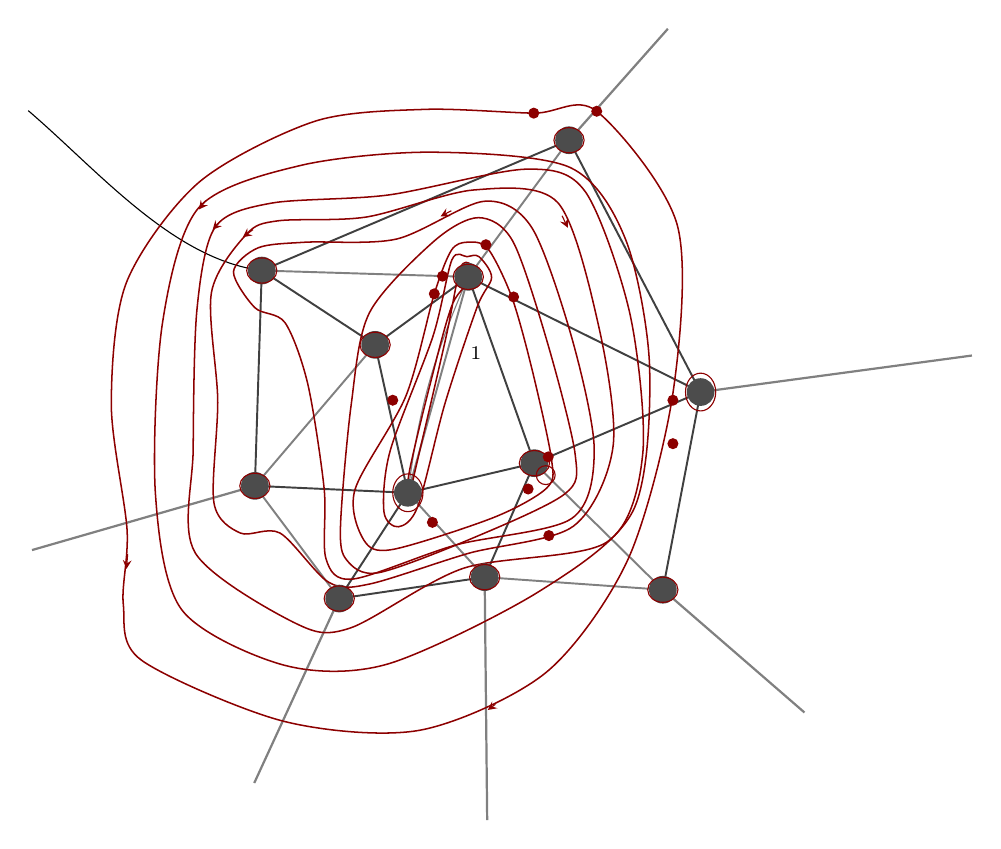
\begin{tikzpicture}[x=.008cm,y=-.008cm,>=stealth]
\coordinate (a) at (585,470);
\coordinate (b) at (1073,263);
\coordinate (c) at (913,480);
\coordinate (d) at (765,588);
\coordinate (e) at (574,812);
\coordinate (f) at (817,823);
\coordinate (g) at (1018,776);
\coordinate (h) at (1282,663);
\coordinate (i) at (708,991);
\coordinate (j) at (939,957);
\coordinate (k) at (1222,977);
\draw[black!75,line width=.7pt] (a)--(b);
\draw[gray,line width=.7pt] (a)--(c);
\draw[black!75,line width=.7pt] (a)--(d);
\draw[black!75,line width=.7pt] (a)--(e);
\draw[gray,line width=.7pt] (b)--(c);
\draw[black!75,line width=.7pt] (b)--(h);
\draw[black!75,line width=.7pt] (c)--(d);
\draw[gray,line width=.7pt] (c)--(f);
\draw[black!75,line width=.7pt] (c)--(g);
\draw[black!75,line width=.7pt] (c)--(h);
\draw[gray,line width=.7pt] (d)--(e);
\draw[black!75,line width=.7pt] (d)--(f);
\draw[black!75,line width=.7pt] (e)--(f);
\draw[gray,line width=.7pt] (e)--(i);
\draw[black!75,line width=.7pt] (f)--(g);
\draw[black!75,line width=.7pt] (f)--(i);
\draw[gray,line width=.7pt] (f)--(j);
\draw[black!75,line width=.7pt] (g)--(h);
\draw[black!75,line width=.7pt] (g)--(j);
\draw[gray,line width=.7pt] (g)--(k);
\draw[black!75,line width=.7pt] (h)--(k);
\draw[black!75,line width=.7pt] (i)--(j);
\draw[gray,line width=.7pt] (j)--(k);
\draw[gray] (c) to[bend right=8] (f);
\draw[gray,line width=.8pt] (b)--(1230,86);
\draw[gray,line width=.8pt] (e)--(220,914);
\draw[gray,line width=.8pt] (i)--(573,1284);
\draw[gray,line width=.8pt] (j)--(943,1343);
\draw[gray,line width=.8pt] (k)--(1447,1172);
\draw[gray,line width=.8pt] (h)--(1713,605);
\draw[black] (a) .. controls (443,452) and (324,310) .. (214,216);
\draw[red!55!black,line width=.55pt] plot[smooth cycle,tension=.5] coordinates {(1117,217) (1245,398) (1238,665) (1167,928) (1037,1108) (837,1200) (620,1186) (394,1089) (365,1000) (371,882) (346,684) (370,489) (485,330) (669,233) (844,214) (1017,220)};
\draw[red!55!black,line width=.55pt] plot[smooth cycle,tension=.5] coordinates {(485,370) (427,555) (416,824) (458,1009) (621,1097) (785,1095) (1025,980) (1175,851) (1201,624) (1163,421) (1074,306) (854,282) (647,303)};
\draw[red!55!black,line width=.55pt] plot[smooth cycle,tension=.5] coordinates {(511,401) (482,532) (476,754) (479,918) (638,1030) (725,1038) (905,943) (1132,902) (1190,762) (1170,540) (1099,345) (1005,309) (786,350) (600,363)};
\draw[red!55!black,line width=.55pt] plot[smooth cycle,tension=.5] coordinates {(561,412) (505,505) (515,676) (509,839) (551,887) (614,887) (691,965) (756,968) (914,919) (1080,876) (1143,749) (1120,558) (1055,362) (922,342) (751,385) (611,391)};
\draw[red!55!black,line width=.55pt] plot[smooth cycle,tension=.5] coordinates {(579,434) (540,472) (574,529) (622,553) (658,650) (684,816) (687,928) (730,960) (893,906) (1077,864) (1113,755) (1078,579) (1014,402) (938,360) (799,420) (654,425)};
\draw[red!55!black,line width=.55pt] plot[smooth cycle,tension=.5] coordinates {(756,537) (727,683) (710,876) (720,930) (770,950) (920,895) (1066,825) (1083,764) (1040,589) (984,424) (929,386) (859,423)};
\draw[red!55!black,line width=.55pt] plot[smooth cycle,tension=.5] coordinates {(859,507) (814,669) (733,818) (747,898) (793,913) (954,862) (1038,815) (1045,769) (1014,626) (982,512) (944,435) (911,425) (886,438)};
\draw[red!55!black,line width=.55pt] plot[smooth cycle,tension=.5] coordinates {(887,453) (857,574) (789,756) (779,853) (802,877) (833,844) (876,681) (927,528) (950,481) (930,448) (911,448)};
\draw[red!55!black,line width=.55pt] plot[smooth cycle,tension=.5] coordinates {(900,467) (878,574) (835,760) (816,838) (820,786) (853,648) (888,523) (923,479) (917,460)};
\fill[black!70] (a) circle (5pt);
\draw[red!55!black] (a) ellipse (24 and 20);
\fill[black!70] (b) circle (5pt);
\draw[red!55!black] (b) ellipse (24 and 20);
\fill[black!70] (c) circle (5pt);
\draw[red!55!black] (c) ellipse (24 and 20);
\fill[black!70] (d) circle (5pt);
\draw[red!55!black] (d) ellipse (24 and 20);
\fill[black!70] (e) circle (5pt);
\draw[red!55!black] (e) ellipse (24 and 20);
\fill[black!70] (f) circle (5pt);
\draw[red!55!black] (f) ellipse (24 and 30);
\fill[black!70] (g) circle (5pt);
\draw[red!55!black] (g) ellipse (24 and 20);
\fill[black!70] (h) circle (5pt);
\draw[red!55!black] (h) ellipse (24 and 30);
\fill[black!70] (i) circle (5pt);
\draw[red!55!black] (i) ellipse (24 and 20);
\fill[black!70] (j) circle (5pt);
\draw[red!55!black] (j) ellipse (24 and 20);
\fill[black!70] (k) circle (5pt);
\draw[red!55!black] (k) ellipse (24 and 20);
\draw[red!55!black] (1036,795) circle (15);
\fill[red!55!black] (1117,217) circle (2pt);
\fill[red!55!black] (1017,220) circle (2pt);
\fill[red!55!black] (941,429) circle (2pt);
\fill[red!55!black] (872,479) circle (2pt);
\fill[red!55!black] (859,507) circle (2pt);
\fill[red!55!black] (985,512) circle (2pt);
\fill[red!55!black] (793,676) circle (2pt);
\fill[red!55!black] (1040,766) circle (2pt);
\fill[red!55!black] (1238,745) circle (2pt);
\fill[red!55!black] (1238,676) circle (2pt);
\fill[red!55!black] (856,870) circle (2pt);
\fill[red!55!black] (1008,817) circle (2pt);
\fill[red!55!black] (1041,891) circle (2pt);
\draw[->,red!55!black] (496,359)--(485,373);
\draw[->,red!55!black] (519,392)--(507,405);
\draw[->,red!55!black] (571,405)--(555,417);
\draw[->,red!55!black] (886,375)--(869,384);
\draw[->,red!55!black] (1062,383)--(1071,402);
\draw[->,red!55!black] (956,1159)--(944,1168);
\draw[->,red!55!black] (372,920)--(370,944);
\node[font=\scriptsize] at (925,601) {$\unsure{1}$};
\end{tikzpicture}}
% crop-candidate: scan 72


\figure{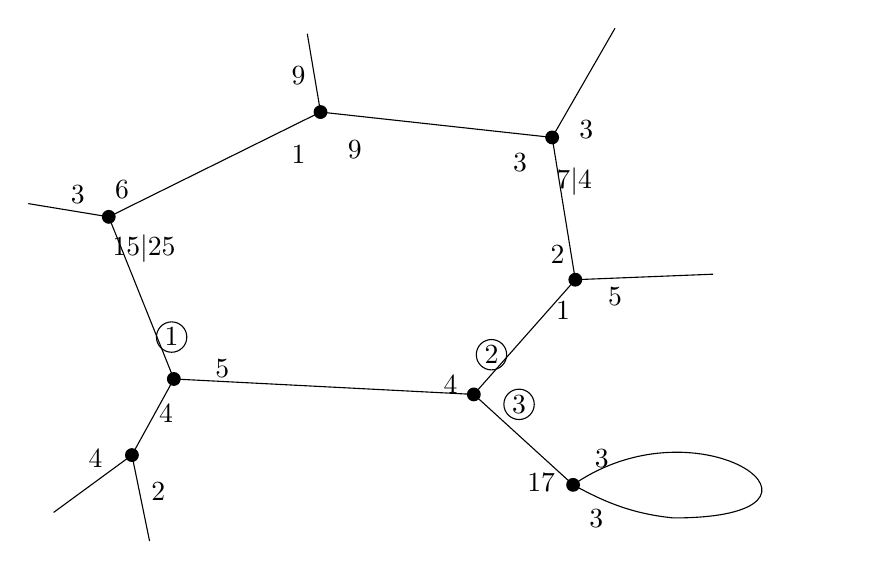
\begin{tikzpicture}[x=.014cm,y=-.014cm]
\coordinate (a) at (1558,821); \coordinate (b) at (1750,726);
\coordinate (c) at (1960,749); \coordinate (d) at (1981,878);
\coordinate (e) at (1889,982); \coordinate (f) at (1617,968);
\coordinate (g) at (1579,1037); \coordinate (h) at (1979,1064);
\draw (a)--(b)--(c)--(d)--(e)--(f)--cycle;
\draw (f)--(g) (e)--(h);
\draw (a)--(1485,809) (b)--(1738,655) (c)--(2017,650);
\draw (d)--(2106,873);
\draw (g)--(1508,1089) (g)--(1595,1115);
\draw (h) .. controls (2096,983) and (2245,1094) .. (2070,1094) .. controls (2030,1090) and (2005,1078) .. (h);
\foreach \p in {a,b,c,d,e,f,g,h} \fill (\p) circle (2.5pt);
\node at (1530,801) {$3$}; \node at (1570,796) {$6$};
\node at (1590,850) {$\unsure{15|25}$};
\node at (1730,693) {$9$}; \node at (1730,765) {$1$}; \node at (1781,760) {$9$};
\node at (1931,772) {$3$}; \node at (1991,742) {$3$}; \node at (1980,789) {$\unsure{7|4}$};
\node at (1965,855) {$2$}; \node at (1970,906) {$1$}; \node at (2017,893) {$5$};
\node at (1868,973) {$4$};
\node[draw,circle,inner sep=1pt] at (1905,946) {$2$};
\node[draw,circle,inner sep=1pt] at (1930,991) {$3$};
\node[draw,circle,inner sep=1pt] at (1615,930) {$1$};
\node at (1661,959) {$5$}; \node at (1610,999) {$4$};
\node at (1546,1040) {$4$}; \node at (1603,1070) {$2$};
\node at (1950,1062) {$17$}; \node at (2005,1040) {$3$}; \node at (2000,1095) {$3$};
\end{tikzpicture}}

\mspage{71}
